\documentclass[rs,english,toc,lot,lof,index,wide,overfull]{prismdoc}
%====================================
% PRISMDOC: Start Dokument Information
%====================================
%\usepackage{longtable}
\usepackage[numbers]{natbib}
\usepackage{verbatim}
\usepackage{epsfig}
\usepackage{rotating}
\usepackage{graphicx}
\usepackage{amssymb}
\usepackage{longtable}
%
% Specifications for cover pages:

\prismdocNum{}
\prismdocTitel{{\fontsize{13}{16}\selectfont
    OASIS3-MCT v6 User Guide \\ TR-CMGC-25-161 \\ [0.5ex]
    }}
\prismdocAutor{Edited by:  \\ [0.5ex]
            S. Valcke, A. Craig, A. Piacentini and G. Jonville \\[0.5ex]
            CECI, Universit\'e de Toulouse, CERFACS \\[0.5ex]
}
%\prismdocVersion{\it{git master branch}}
\prismdocSName{Sophie Valcke}
\prismdocFAff{CNRS}
\prismdocSAff{CERFACS}
%\prismdocFEM{toto}
\prismdocFEm{oasishelp(at)cerfacs.fr}
\prismdocFName{Laure Coquart}
\prismdocSPhone{}
\prismdocFPhone{}
%\prismdocFWp{wpnn}
%\prismdocSWp{wpnn}
\prismdocDate{December 15, 2025}


%====================================
% PRISMDOC: End Dokument Information
%====================================
\newcommand{\antispace}{\vspace*{-2ex}}
\newcommand{\bigspace}{\vspace*{+4ex}}
%\newcommand{\medspace}{\vspace*{+2ex}}
\newcommand{\smallspace}{\vspace*{+0ex}}
\newcommand{\marginlabel}[1]{\mbox{}\marginpar{\raggedleft\hspace{0pt}#1}}
\newcommand{\imprt}{\marginlabel{{\bfseries\Huge !}}}
\newcommand{\imprtbig}{\marginlabel{{\bfseries\Huge !}}}
\newcommand{\bignote}{\marginlabel{{\bfseries\Huge !!!}}}
\newcommand{\imprtsm}{\marginlabel{{\bfseries\LARGE !}}}
\newcommand{\imnote}{\marginlabel{{\bfseries\LARGE !!!}}}
\newcommand{\bcntr}{\begin{center}}
\newcommand{\ecntr}{\end{center}}

%\includeonly{documentation}
\begin{document}
%\setcounter{secnumdepth}{-1}
\prismdocHeader

\include{defines}
\include{UG_Acknowledgements}
\newpage
\chapter{Introduction}
\label{sec_step}

In 1991, CERFACS started the development of
a software interface to couple existing ocean and atmosphere numerical General
Circulation Models. Today, different versions of the 
OASIS3-MCT coupler are used by at least 65 modelling groups all around the
world to couple more than 80 applications on different computing platforms\footnote{A list of
coupled models realised with OASIS3-MCT can be found at https://oasis.cerfacs.fr/en/oasis-coupled-models/}.
OASIS3-MCT sustained development is ensured by a collaboration
between CERFACS and the Centre National de la Recherche Scientifique
(CNRS) and its maintenance and user support is regularly reinforced
with additional resources coming from European and national projects.

OASIS3-MCT is a portable set of Fortran 77, Fortran 90 and C
routines. Low-intrusiveness, portability and flexibility are
OASIS3-MCT key design concepts. After compilation OASIS3-MCT is a
coupling library to be linked to the component models, and which main
function is to interpolate and exchange the coupling fields between the components to form a coupled system.  OASIS3-MCT supports  coupling of 2D
logically-rectangular fields but 3D fields and 1D fields expressed on
unstructured grids are also supported using a one dimension
degeneration of the structures.

Internally, OASIS3-MCT uses MCT, the Model
Coupling Toolkit\footnote{https://web.cels.anl.gov/projects/climate/mct/} \citep{mct_larson} \citep{mct_jacob}, 
developed by the Argonne National Laboratory in the USA. MCT implements fully parallel remapping, as a parallel matrix vector 
multiplication on the set of source or
target component processes, and parallel distributed exchanges of the coupling
fields via Message Passing Interface
(MPI). 
Its design philosophy, based on flexibility and minimal invasiveness,
is close to the OASIS3-MCT approach. 

To communicate with another component, a component model needs to include few specific calls to OASIS3-MCT Fortran Application Programming Interface (API).  OASIS3-MCT also has python and C language bindings. For remapping the coupling fields from the source to the target grid, OASIS3-MCT\_6.0 includes a modified version of the SCRIP library \citep{Jones99} and is interfaced with YAC version 3.10 \citep{hanke2016} \citep{hanke2019} \cite{jonville2024}. OASIS3-MCT also supports basic non-parallel file I/O using NetCDF .  The configuration of the coupling exchanges needs to be described externally by the user in a text file, the {\it namcouple}. 

The developments realised between the different versions of OASIS3-MCT are described in Appendix \ref{sec_changes}.

We believe that OASIS3-MCT will still provide an efficient and
easy-to-use coupling solution for many climate modelling groups in the few years to come. 

%See appendix \ref{sec_changes} for a more detailed list of changes in this %version.

\section{Step-by-step use of OASIS3-MCT}

To use OASIS3-MCT for coupling codes, one has to follow these steps:
\begin{enumerate}
\item Obtain OASIS3-MCT source code (see chapter \ref{sec_Obtaining}).
\item Get familiar with OASIS3-MCT, either by following the Short Private Online Course (SPOC, see  https://cerfacs.fr/en/online-traning-sessions/ ) or by going through the tutorial steps. A tutorial is also available in directory {\tt
  examples/tutorial\_communication} and all explanations are provided in the document
{\tt tutorial\_communication.pdf} therein.

\item Identify the coupling or I/O fields and adapt the codes to
  implement the coupling exchanges with the OASIS3-MCT coupling library based on MPI message passing.
  The OASIS3-MCT coupling library uses NetCDF and therefore can also be used to perform I/O actions
  from/to disk files.  For more detail on how to use the 
  OASIS3-MCT API in the codes, see chapter \ref{sec_modelinterfacing}.

\item Define all coupling and I/O parameters and transformations
  required to adapt each coupling field from the source model grid to
  the target model grid. On this basis, prepare OASIS3-MCT configuring file 
  {\it namcouple}.
  OASIS3-MCT supports different interpolation algorithms as described in
  chapter \ref{sec_transformations}.  Remapping files can be computed
  online using the SCRIP or YAC library, or offline using either the SCRIP, YAC, ESMF or XIOS (see  {\tt
  examples/regrid\_environment}, section \ref{subsec_regrid}) and read in during the run using the MAPPING
  transformation.

{\bf We strongly recommend to tests the quality of the chosen transformations and remappings} off-line using the environment available in {\tt
  examples/regrid\_environment} and explanations provided in the document {\tt regrid\_environment.pdf} therein. 

\item Generate required auxiliary data files , if needed (see chapter
  \ref{sec_auxiliary}).
\item Compile OASIS3-MCT, the component models and start the coupled
  experiment. For details on how to compile and run a coupled model
  with OASIS3-MCT, see section \ref{sec_compilationrunning}. 

\end{enumerate}

If you need extra help, do not hesitate to contact us at
oasishelp(at)cerfacs.fr .

\section{OASIS3-MCT sources}
\label{sec_Obtaining}
OASIS3-MCT sources are available from CERFACS git server. To obtain more detail on downloading
the sources, please fill in the registration form at https://oasis.cerfacs.fr/en/downloads/ .

OASIS3-MCT directory structure is the following one:

\begin{verbatim}
 - oasis3-mct/lib/cbindings        C language bindings source code
                 /mct              Model Coupling Toolkit Coupling Software
                 /psmile           OASIS3-MCT coupling library
                 /scrip            SCRIP remapping library  
                 /yac              YAC  remapping library 
                 /yaxt	            communication layer used by YAC            

 - oasis3-mct/doc                  OASIS3-MCT User Guide

 - oasis3-mct/util/make_dir        Utilities to compile OASIS3-MCT
                  /load_balancing  Tool for load balancing analysis
                  /env_tests        Script to compile and launch toy models          
                  
 - oasis3-mct/pyoasis	             Python wrapper source code

 - oasis3-mct/examples             Environment to compile, run and use
                                   different toy coupled models. 
\end{verbatim}
\newpage
\section{Licenses and Copyrights}
 
\subsection{OASIS3-MCT license and copyright statement}

Copyright © 2025 Centre Europ\'een de Recherche et Formation
Avanc\'ee en Calcul Scientifique (CERFACS).  

This software and ancillary information called OASIS3-MCT is free
software.  CERFACS has rights to use, reproduce, and distribute
OASIS3-MCT. The public may copy, distribute, use, prepare derivative works and
publicly display OASIS3-MCT under the terms of the Lesser GNU General
Public License (LGPL) as published by the Free Software Foundation,
provided that this notice and any statement of authorship are
reproduced on all copies. If OASIS3-MCT is modified to produce derivative
works, such modified software should be clearly marked, so as not to
confuse it with the OASIS3-MCT version available from CERFACS.

The developers of the OASIS3-MCT software are researchers attempting to
build a modular and user-friendly coupler accessible to the climate
modelling community. Although we use the tool ourselves and have made
every effort to ensure its accuracy, we can not make any
guarantees. We provide the software to you for free. In return,
you --the user-- assume full responsibility for use of the software. The
OASIS3-MCT software comes without any warranties (implied or expressed) and
is not guaranteed to work for you or on your computer. Specifically,
CERFACS and the various individuals involved in development and
maintenance of the OASIS3-MCT software are not responsible for any damage
that may result from correct or incorrect use of this software.

\subsection{MCT copyright statement}
\label{sec_MCT}

                            Modeling Coupling Toolkit (MCT) Software

Copyright © 2021, UChicago Argonne, LLC as Operator of Argonne National Laboratory. All rights reserved.

Redistribution and use in source and binary forms, with or without modification, are permitted provided that the following conditions are met:
\begin{enumerate}
\item Redistributions of source code must retain the above copyright notice, this list of conditions and the following disclaimer.
\item Redistributions in binary form must reproduce the above copyright notice, this list of conditions and the following disclaimer in the documentation and/or other materials provided with the distribution.
\item The end-user documentation included with the redistribution, if any, must include the following acknowledgment: "This product includes software developed by the UChicago Argonne, LLC, as Operator of Argonne National Laboratory." Alternately, this acknowledgment may appear in the software itself, if and wherever such third-party acknowledgments normally appear.

This software was authored by:
\begin{itemize}
\item Argonne National Laboratory Climate Modeling Group, Mathematics and Computer Science Division, Argonne National Laboratory, Argonne IL 60439
\item Robert Jacob, tel: (630) 252-2983, E-mail: jacob@mcs.anl.gov
\item Jay Larson, E-mail: larson@mcs.anl.gov
\item Everest Ong
\item Ray Loy
\end{itemize}

\item WARRANTY DISCLAIMER. THE SOFTWARE IS SUPPLIED "AS IS" WITHOUT WARRANTY OF ANY KIND. THE COPYRIGHT HOLDER, THE UNITED STATES, THE UNITED STATES DEPARTMENT OF ENERGY, AND THEIR EMPLOYEES: (1) DISCLAIM ANY WARRANTIES, EXPRESS OR IMPLIED, INCLUDING BUT NOT LIMITED TO ANY IMPLIED WARRANTIES OF MERCHANTABILITY, FITNESS FOR A PARTICULAR PURPOSE, TITLE OR NON-IN- FRINGEMENT, (2) DO NOT ASSUME ANY LEGAL LIABILITY OR RESPONSIBILITY FOR THE ACCURACY, COMPLETENESS, OR USEFULNESS OF THE SOFTWARE, (3) DO NOT REPRESENT THAT USE OF THE SOFTWARE WOULD NOT INFRINGE PRIVATELY OWNED RIGHTS, (4) DO NOT WARRANT THAT THE SOFTWARE WILL FUNCTION UNINTERRUPTED, THAT IT IS ERROR-FREE OR THAT ANY ERRORS WILL BE CORRECTED. 

\item LIMITATION OF LIABILITY. IN NO EVENT WILL THE COPYRIGHT HOLDER, THE UNITED STATES, THE UNITED STATES DEPARTMENT OF ENERGY, OR THEIR EMPLOYEES: BE LIABLE FOR ANY INDIRECT, INCIDENTAL, CONSEQUENTIAL, SPECIAL OR PUNITIVE DAMAGES OF ANY KIND OR NATURE, INCLUDING BUT NOT LIMITED TO LOSS OF PROFITS OR LOSS OF DATA, FOR ANY REASON WHATSOEVER, WHETHER SUCH LIABILITY IS ASSERTED ON THE BASIS OF CONTRACT, TORT (INCLUDING NEGLIGENCE OR STRICT LIABILITY), OR OTHERWISE, EVEN IF ANY OF SAID PARTIES HAS BEEN WARNED OF THE POSSIBILITY OF SUCH LOSS OR DAMAGES.

\end{enumerate}

\subsection{SCRIP 1.4 license copyright statement}
\label{sec_SCRIP}

Copyright © 1997, 1998 the Regents of the University of California.
This software and ancillary information (herein called SOFTWARE)
called SCRIP is made available under the terms described here. The
SOFTWARE has been approved for release with associated LA-CC Number
98-45. Unless otherwise indicated, this SOFTWARE has been authored by
an employee or employees of the University of California, operator of
Los Alamos National Laboratory under Contract No. W-7405-ENG-36 with
the United States Department of Energy. The United States Government
has rights to use, reproduce, and distribute this SOFTWARE. The public
may copy, distribute, prepare derivative works and publicly display
this SOFTWARE without charge, provided that this Notice and any
statement of authorship are reproduced on all copies. Neither the
Government nor the University makes any warranty, express or implied,
or assumes any liability or responsibility for the use of this
SOFTWARE. If SOFTWARE is modified to produce derivative works, such
modified SOFTWARE should be clearly marked, so as not to confuse it
with the version available from Los Alamos National Laboratory.

\subsection{YAC license copyright statement}
\label{sec_YAC}

Copyright (c) 2025 The YAC Authors

SPDX-License-Identifier: CC-BY-4.0
%\include{UG1_Obtaining}
\newpage
\chapter{Interfacing a component code with OASIS3-MCT}
\label{sec_modelinterfacing}

At run-time, OASIS3-MCT performs parallel exchange of coupling data between parallel
components and sub-components and allows remapping (interpolation), time integration or accumulation and other transformations of these coupling fields. 

This chapter describes how to adapt the component codes to couple them through OASIS3-MCT. 

OASIS3-MCT supports coupling exchanges between parallel
components and sub-components deployed in diverse
configurations; the different possibilities and how to use
the OASIS3-MCT library accordingly are described in section
\ref{sec_deploy}. 

The OASIS3-MCT Application Programming Interface (API) includes different classes of modules or routines that are described in details in sections \ref{API}, \ref{APIC} and \ref{APIpython} for Fortran, C and python codes respectively.
In section \ref{sec_notes}, the reader will also find an overview of the MCT library (see \ref{subsec_MCT}) and additional notes on how to exchange scalars (see \ref{subsec_scalar}), how to to reproduce different coupling
algorithms with OASIS3-MCT using the {\tt LAG} index (see \ref{subsec_lag}), and on the {\tt
  SEQ} index (see \ref{subsec_sec}).

\section{Configurations of components supported}
\label{sec_deploy}

Since OASIS3-MCT\_3.0 release, coupling exchanges between components and
sub-components deployed in a much larger diversity of configurations
are supported. This is illustrated on figure
\ref{Fig_coupling_layouts_a} and how to use the OASIS3-MCT library
accordingly is detailed on figure \ref{Fig_coupling_layouts_b}. All
OASIS3-MCT API routines are also described in details in sections
\ref{API}, \ref{APIC} and \ref{APIpython}. 

We call here an ``executable'' a compiled code
  forming a part of or the whole coupled system (started with the
  mpirun or mpiexec command). A ``component'' is the ensemble of
  processes, or tasks, within the coupled system calling {\tt oasis\_init\_comp}
  with the same {\tt comp\_name} argument (see section
  \ref{init_comp}). A ``sub-component'' is the subset of tasks within a
  component sending or receiving coupling fields on a specific grid;
  of course, a component may have only one sub-component
  that gathers all its tasks.

Practical examples of how to use the OASIS3-MCT library are also given in {\tt examples/} {\tt tutorial} and {\tt examples/test\_1bin\_ocnice} (see sections \ref{subsec_tutorial} and \ref{subsec_1bin_ocnice}).XXXXXXXXXXXXXX 

Since OASIS3-MCT\_3.0, it is possible to (the text between [ and ] refers to figure \ref{Fig_coupling_layouts_a}) :

\begin{figure}
  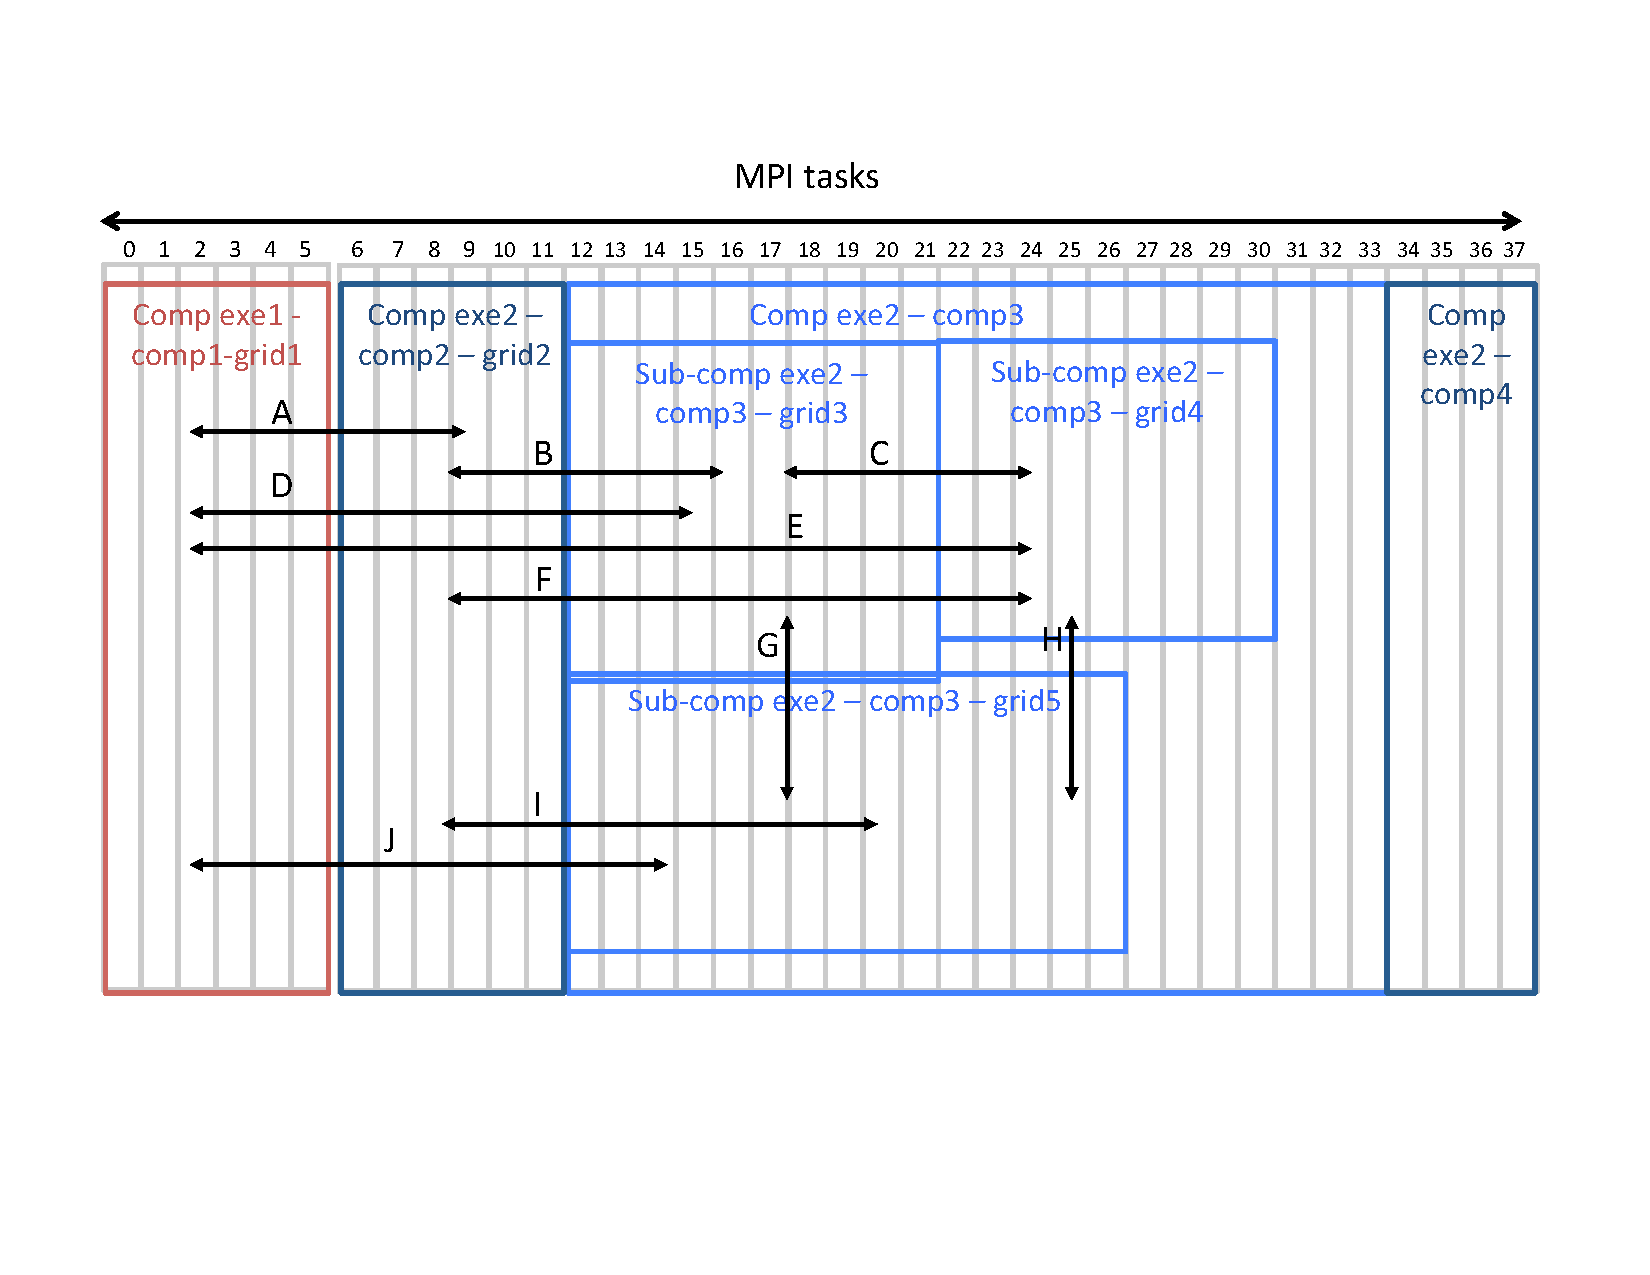
\includegraphics[scale=.6]{figures/coupling_layouts_a}
  \caption{The different configuration of components supported by OASIS3-MCT\_3.0. Two executables {\tt exe1} and {\tt exe2} are running concurrently on separate sets of MPI tasks (0-5 for {\tt exe1} and 6-37 for {\tt exe2}). Executable {\tt exe1} includes only one component {\tt comp1} that has coupling fields defined on only one grid {\tt grid1} (decomposed on all its 6 tasks). Executable {\tt exe2} includes 3 components, {\tt comp2}, {\tt comp3}, and {\tt comp4} running concurrently respectively on tasks 6-11, 12-33 and 34-37. Component {\tt comp2} participates in the coupling with fields defined on only one coupling grid {\tt grid2} (decomposed on all its 5 tasks) while {\tt comp4} does not participate at all in the coupling. 
Component {\tt comp3} has 3 sub-components, respectively exchanging
coupling fields defined on {\tt grid3} (tasks 12-21), {\tt grid4}
(tasks 22-30) and {\tt grid5} (tasks 12-26, therefore overlaping with both {\tt
  grid3} and {\tt grid4}); finally, {\tt comp3} has 3 tasks (31-33)
not involved in the coupling. Sub-components exe2-comp3-grid3 and
exe2-comp3-grid5, or sub-components exe2-comp3-grid4 and
exe2-comp3-grid5 are examples of coupling between sub-components running sequentially on overlapping sets of tasks.}
  \label{Fig_coupling_layouts_a}
\end{figure}

\begin{figure}
  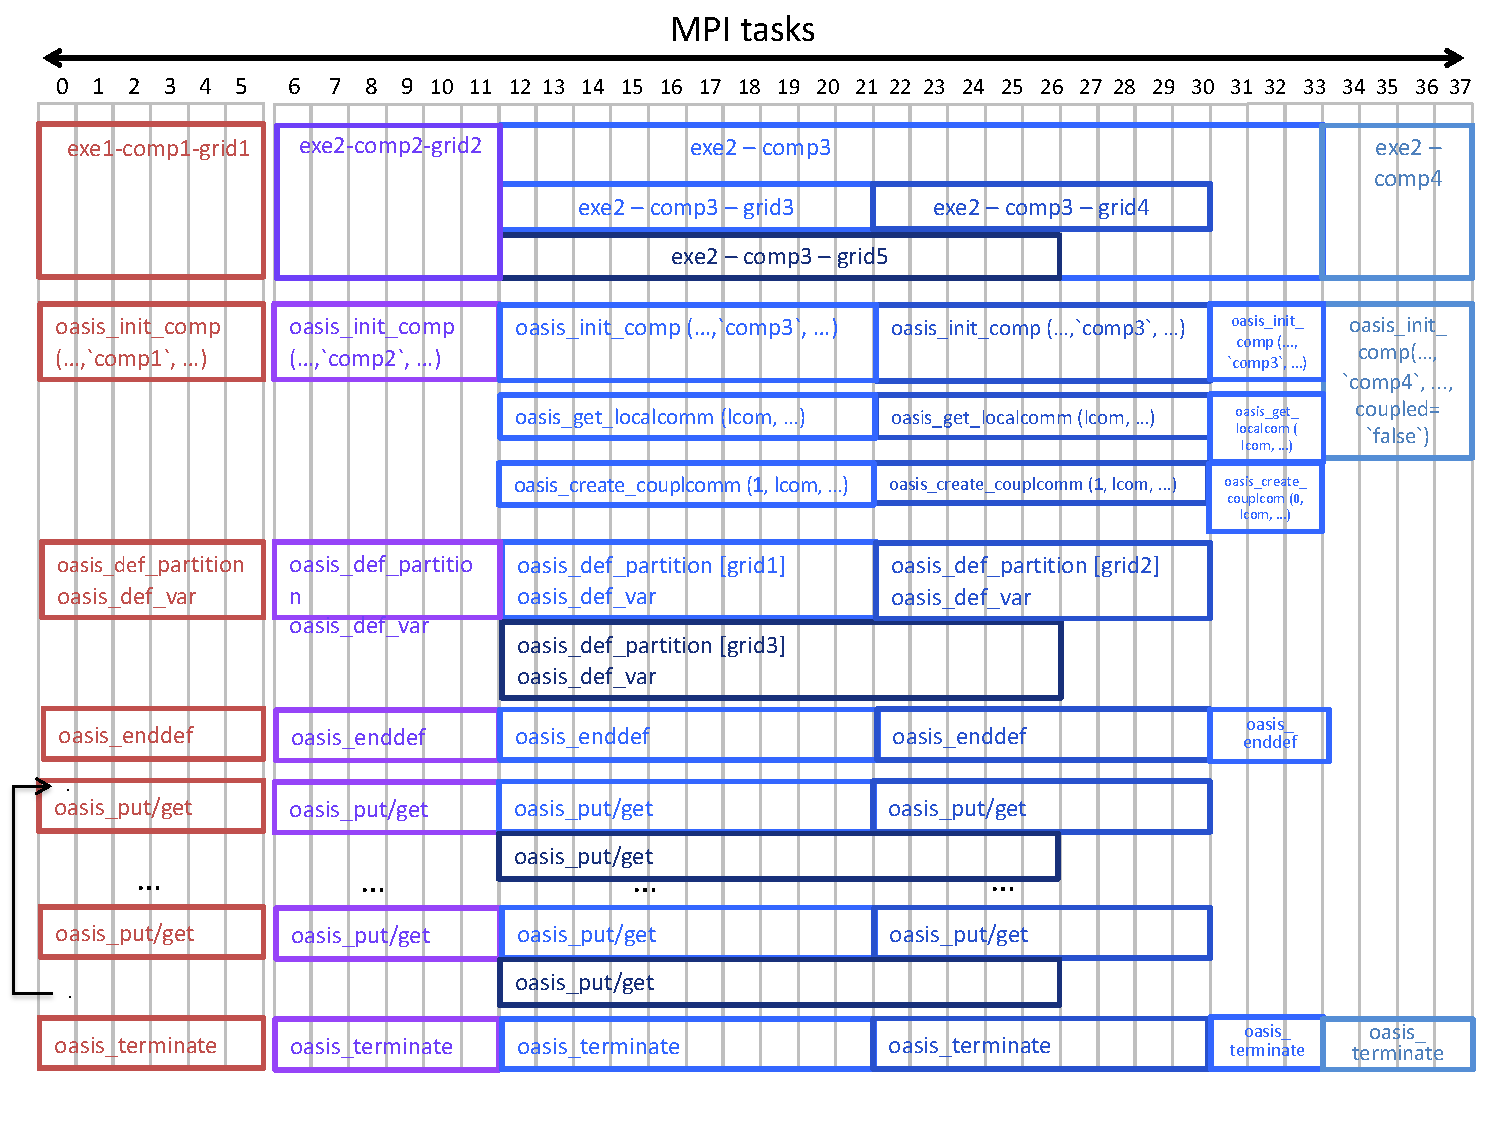
\includegraphics[scale=.6]{figures/coupling_layouts_b}
  \caption{The sequence of OASIS3-MCT calls that have to be implemented in the codes so to allow the configuration of components described on figure \ref{Fig_coupling_layouts_a}.
Each MPI tasks has to call {\tt oasis\_init\_comp} once with the name
of its component as $2^{nd}$ argument. As none of {\tt comp4} tasks is
participating to the coupling, {\tt comp4} tasks calls {\tt
  oasis\_init\_comp} with {\tt coupled=.false.”} as $4^{th}$ argument
and does not call any other OASIS3-MCT routine. As some of {\tt comp3}
tasks are participating to the coupling, all {\tt comp3} tasks have to
call {\tt oasis\_init\_comp}, {\tt oasis\_get\_localcomm}, {\tt
  oasis\_create\_couplcomm}, {\tt oasis\_enddef} and {\tt
  oasis\_terminate} (these are the only routine to be called by {\tt
  comp3} tasks 31-33 not participating to the coupling). To initialise
the coupling exchanges, the tasks of a sub-component holding a field
decomposed on a specific grid have to call the {\tt
  oasis\_def\_partition} to express the decomposition of the grid,
{\tt oasis\_def\_var} to declare the coupling field and {\tt
  oasis\_enddef}. Finally, the tasks of a sub-component exchanging 
coupling fields have to call {\tt oasis\_put} and {\tt oasis\_get} accordingly.
}
  \label{Fig_coupling_layouts_b}
\end{figure}

\begin{itemize}

\item to implement coupling exchanges between two components or
  sub-components running concurrently on separate sets of tasks within two different executables  (as before) [A, D, E, J];
\item to implement coupling exchanges between two components or
  sub-components running concurrently on separate sets of tasks within one same executable [B, F, I];
\item to implement coupling exchanges within one executable between
  two concurrent sub-components [C] 
\item to implement coupling exchanges within one executable between
  two sub-components running sequentially on overlapping sets of tasks (i.e. a task can be coupled to itself calling both the ``put” and the ``get” of the exchange) [G, H]
\item to have some tasks of a component not participating to the coupling exchanges [tasks 31-33 of {\tt exe2-comp3}]
\item to have all processes of a component not participating to the coupling exchanges [{\tt exe2-comp4}, tasks 34-37]

\end{itemize}

The sequence of OASS3-MCT API routines that have to be called in the different cases is detailed on figure  \ref{Fig_coupling_layouts_b}.  These routines are also described in detail in the next section.

\section{OASIS3-MCT Fortran API}
\label{API}

To interact with the rest of the coupled system, few calls of the
OASIS3-MCT library routines, which sources can be found in {\tt
  oasis3-mct/lib/psmile} directory, have to be implemented in
component Fortran codes. They belong to the following classes:
\begin{enumerate}
\item Module to use (section \ref{subsubsec_Use})
\item Initialisation (section \ref{subsubsec_Initialisation})
\item Partition definition (section \ref{subsubsec_Partition})
\item Grid data file definition (section \ref{subsubsec_griddef})
\item Coupling-I/O field declaration (section
  \ref{subsubsec_Declaration})
\item End of definition phase (section
  \ref{subsubsec_Endofdefinition})
\item Coupling-I/O field sending and receiving (section
  \ref{subsubsec_sendingreceiving})
\item Termination (section \ref{subsubsec_Termination})
\item Optional auxiliary routines (section
  \ref{subsubsec_auxroutines})
\end{enumerate}

\subsection{Module to use in the code}
\label{subsubsec_Use}
% {Use}

To use OASIS3-MCT library, a user needs to add in his code:

\begin{itemize}

\item {\tt USE mod\_oasis}

  or

\item {\tt USE mod\_prism}
 
\end{itemize}

Both use statements are valid but only one needs to be used in a particular component. This single use statement provides all methods required. The methods, datatypes, and capabilities
are identical for both the {\tt mod\_prism} or {\tt mod\_oasis}
interfaces, the only difference being the name of the interface. The
interface in module {\tt mod\_prism} is provided for backwards
compatability with prior versions of OASIS3. Use of module {\tt
  mod\_oasis} is recommended and provides access to a set of updated
routine names that will continue to evolve in the future, always
ensuring backward compatibility.  In the following sections, both the
{\tt mod\_prism} and {\tt mod\_oasis} interface names are defined and
a single description of the interface arguments is provided.

\subsection{Initialisation}
\label{subsubsec_Initialisation}
% {Initialisation}

\subsubsection{Coupling initialisation}
\label{init_comp}

\begin{itemize}

\item {\tt CALL oasis\_init\_comp (compid, comp\_name, kinfo, coupled, commworld)}
\item {\tt CALL prism\_init\_comp\_proto (compid, comp\_name, kinfo, coupled, commworld)}

  \begin{itemize}
  \item {\tt compid [INTEGER; OUT]}: returned component ID
  \item {\tt comp\_name [CHARACTER; IN]}: component name; maximum length of 80 characters 
  \item {\tt kinfo [INTEGER; OUT]}: returned error code
  \item {\tt coupled [LOGICAL, OPTIONAL; IN]}: flag to specify if the calling task is participating or not to the coupling ({\tt .true.} by default). 
  \item {\tt commworld [INTEGER, OPTIONAL; IN]} : optional argument to specify the global communicator gathering the components of the coupled model. 
  If not specified, {\tt MPI\_COMM\_WORLD} will be used as the default communicator to startup. All components of the coupled model must 
  specify the same {\tt commworld} argument.

  \end{itemize}
 
  This routine must called by all tasks of all components whether of not they are involved in the coupling \footnote{The component may also call MPI\_Init explicitly, but if so, has to call it before calling {\tt oasis\_init\_comp}; in this case, the component also has to call MPI\_Finalize explicitly, but only after calling {\tt oasis\_terminate}.}. 

A component is defined as the ensemble of tasks  calling {\tt
  oasis\_init\_comp} with the same {\tt comp} {\tt \_name}
argument. If and only if all tasks of a component are excluded from
the coupling, the logical {\tt coupled} can be set to {\tt .false.}
for this component tasks; in this case, {\tt oasis\_init\_comp} is the
only API routine that needs to be called by the component tasks. If at
least one tasks of a component is participating to the coupling, all
component tasks have to call {\tt oasis\_init\_comp} with {\tt
  coupled=.true.} (by default); in this case, the component tasks not
participating to the coupling will also have to call
{\tt oasis\_get\_localcomm}, {\tt oasis\_create\_couplcomm}, {\tt oasis\_enddef} and {\tt oasis\_terminate}.
\end{itemize}

\subsubsection{Communicator for internal parallelisation}
\label{subsec_MPI1}

\begin{itemize}
\item {\tt CALL oasis\_get\_localcomm (local\_comm, kinfo )}
\item {\tt CALL prism\_get\_localcomm\_proto (local\_comm, kinfo )}

  \begin{itemize}
  \item {\tt local\_comm [INTEGER; OUT]}: value of local communicator
  \item {\tt kinfo [INTEGER; OUT]}: returned error code.
  \end{itemize}

  This routine returns the value of a local communicator gathering
  only the tasks of the component, i.e. the tasks that called {\tt
  oasis\_init\_comp} with the same {\tt comp\_name}
argument.

  This may be needed as all executables of the coupled system are started in a pseudo-MPMD
  mode with MPI1 and therefore share automatically the same MPI\_COMM\_WORLD
  communicator.  Another communicator has to be used for the internal
  parallelisation of each component. OASIS3-MCT creates this local
  communicator {\tt local\_comm} based on the value of the {\tt
    comp\_name} argument in the {\tt oasis\_init\_comp} call.

  Retrieving a local communicator {\tt local\_comm} is also needed if
  {\tt oasis\_create\_couplcomm} is called, as {\tt local\_comm} is an argument of this routine (see below).

  % With CLIM-MPI2, OASIS3 executable spawns the component
  % executables at the beginning of the run; the components keep their
  % internal parallelisation context unchanged with respect to their
  % standalone mode. In this case, calling the
  % prism\_get\_localcomm\_proto routine is useless but if called, the
  % communicator MPI\_COMM\_WORLD will be returned as local
  % communicator.
\end{itemize}

\begin{itemize}
\item {\tt CALL oasis\_create\_couplcomm(icpl, local\_comm,
    coupl\_comm, kinfo)}
\item {\tt CALL prism\_create\_couplcomm(icpl, local\_comm,
    coupl\_comm, kinfo)}
  \begin{itemize}
  \item {\tt icpl [INTEGER; IN]}: coupling process flag
  \item {\tt local\_comm [INTEGER; IN]}: MPI communicator with all
    processes of the component
  \item {\tt coupl\_comm [INTEGER; OUT]}: returned MPI communicator
    gathering only component processes participating in the coupling
  \item {\tt kinfo [INTEGER; OUT; OPTIONAL]}: returned error code
  \end{itemize}

  This routine creates a coupling communicator for a subset of
  processes. It is mandatory to call this routine if only a subset of
  the component processes participate in the coupling (e.g. {\tt comp3} in figure
    \ref{Fig_coupling_layouts_b}); in that case, the processes
    involved in the coupling have to call it with icpl=1 while the
    other have to call it with icpl = MPI UNDEFINED. Argument
    local\_comm is the MPI communicator associated with all processes
    of the component returned by oasis\_get\_localcomm. The new coupling 
    communicator is returned in coupl\_comm.

\end{itemize}
If this communicator already exists in the code, the component should
simply provide it to OASIS3-MCT with:

\begin{itemize}
\item {\tt CALL oasis\_set\_couplcomm(coupl\_comm, kinfo)}
\item {\tt CALL prism\_set\_couplcomm(coupl\_comm, kinfo)}
  \begin{itemize}
  \item {\tt coupl\_comm [INTEGER; IN]}: MPI communicator gathering
    only component processes participating in the coupling
  \item {\tt kinfo [INTEGER; OUT; OPTIONAL]}: returned error code
  \end{itemize}

  This routine allows to provide a local coupling communicator to
  OASIS3-MCT, given that it already exists in the code. The value of
  {\tt coupl\_comm} must be the value of this local coupling
  communicator for the processes participating to the coupling and it
  must be {\tt MPI\_COMM\_NULL} for processes not involved in the
  coupling.
\end{itemize}

\subsection{Partition definition}
\label{subsubsec_Partition}

The coupling fields sent or received by a component are usually
scattered among the different component processes. With OASIS3-MCT,
all processes exchanging coupling data have to express in a global index space the local
partitioning of the different grids onto which the data is expressed (see \ref{subsubsec_griddef} for the grid definition).
The processes not implied in the
coupling do not have to call this routine (for backward compatibility with OASIS3-MCT\_2.0,
they may still call it describing a null partition, i.e. with {\tt ig\_paral(:)=0}).

\begin{itemize}

  \vspace{0.2cm}
\item {\tt CALL oasis\_def\_partition (il\_part\_id, ig\_paral,
    kinfo, ig\_size, name)} or
\item {\tt CALL prism\_def\_partition\_proto (il\_part\_id, ig\_paral,
    kinfo, ig\_size, name)}

  \begin{itemize}
  \item {\tt il\_part\_id [INTEGER; OUT]}: partition ID
  \item {\tt ig\_paral [INTEGER, DIMENSION(:), IN]}: vector of
    integers describing the local grid partition in the global index space;
    has a different expression depending on the type of the partition;
    in OASIS3-MCT, 5 types of partition are supported: Serial (no
    partition), Apple, Box, Orange, and Points (see below).
  \item {\tt kinfo [INTEGER; OUT]}: returned error code.
  \item {\tt ig\_size [INTEGER, OPTIONAL, IN]}: Optional argument, mandatory
    if the coupling data is exchanged for only a subdomain of the
    global grid; in this case, {\tt ig\_size} must give the total number of grid points.  
  \item {\tt name [CHARACTER, OPTIONAL, IN]}: Optional argument associating a name to the partition,
    mandatory if oasis\_def\_partition is called either for a grid
    decomposed not across all the processes of a component or if the related
    oasis\_def\_partition are not
    called in the same order on the different component processes;
    this argument is new since OASIS3-MCT\_3.0 and is linked to the
    greater flexibility in the configuration of components supported
    (see \ref{sec_deploy}); it has a maximum length of 120 characters. 
  \end{itemize}
\end{itemize}

\subsubsection{Serial (no partition)}

This is the choice for a grid entirely supported by only one process . In this case, we have {\tt
  ig\_paral(1:3)}:
\begin{itemize}
\item {\tt ig\_paral(1)} = 0 (indicates a Serial ``partition'')
\item {\tt ig\_paral(2)} = 0
\item {\tt ig\_paral(3)} = the total grid size.
\end{itemize}

\subsubsection{Apple partition}

Each partition is a segment of the global domain, described by its
global offset and its local size. In this case, we have {\tt
  ig\_paral(1:3)}:
\begin{itemize}
\item {\tt ig\_paral(1)} = 1 (indicates an Apple partition)
\item {\tt ig\_paral(2)} = the segment global offset
\item {\tt ig\_paral(3)} = the segment local size
\end{itemize}

Figure \ref{apple_partition} illustrates an Apple partition over 3
processes.
\begin{figure}
  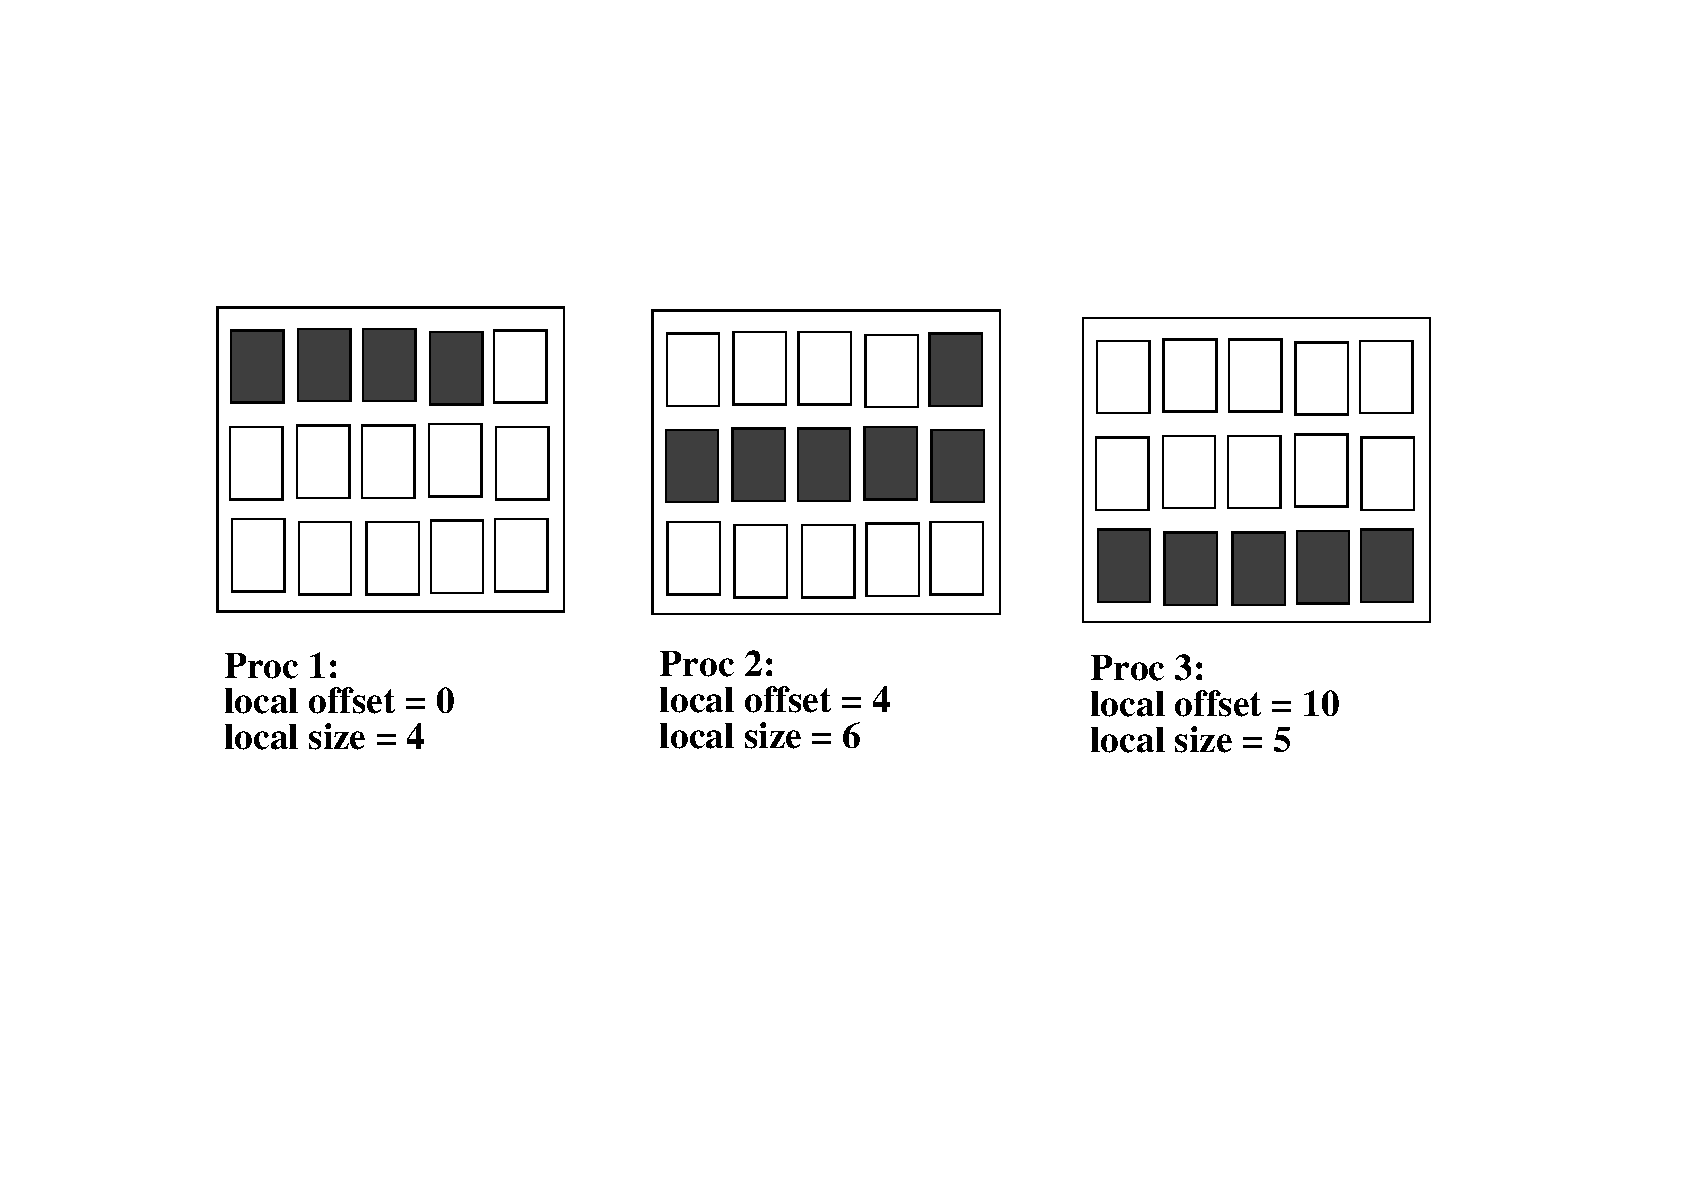
\includegraphics[scale=.6]{figures/apple_new}
  \caption{Apple partition. It is assumed here that the global index starts at
    0 in the upper left corner.}
  \label{apple_partition}
\end{figure}


\subsubsection{Box partition}

Each partition is a rectangular region of the global domain, described
by the global offset of its upper left corner, and its local extents
in the X and Y dimensions. The global extent in the X dimension must
also be given. In this case, we have {\tt ig\_paral(1:5)}:
\begin{itemize}
\item {\tt ig\_paral(1)} = 2 (indicates a Box partition)
\item {\tt ig\_paral(2)} = the upper left corner global offset
\item {\tt ig\_paral(3)} = the local extent in x
\item {\tt ig\_paral(4)} = the local extent in y
\item {\tt ig\_paral(5)} = the global extent in x.
\end{itemize}

Figure \ref{box_partition} illustrates a Box partition over 3
processes.
 
\begin{figure}
  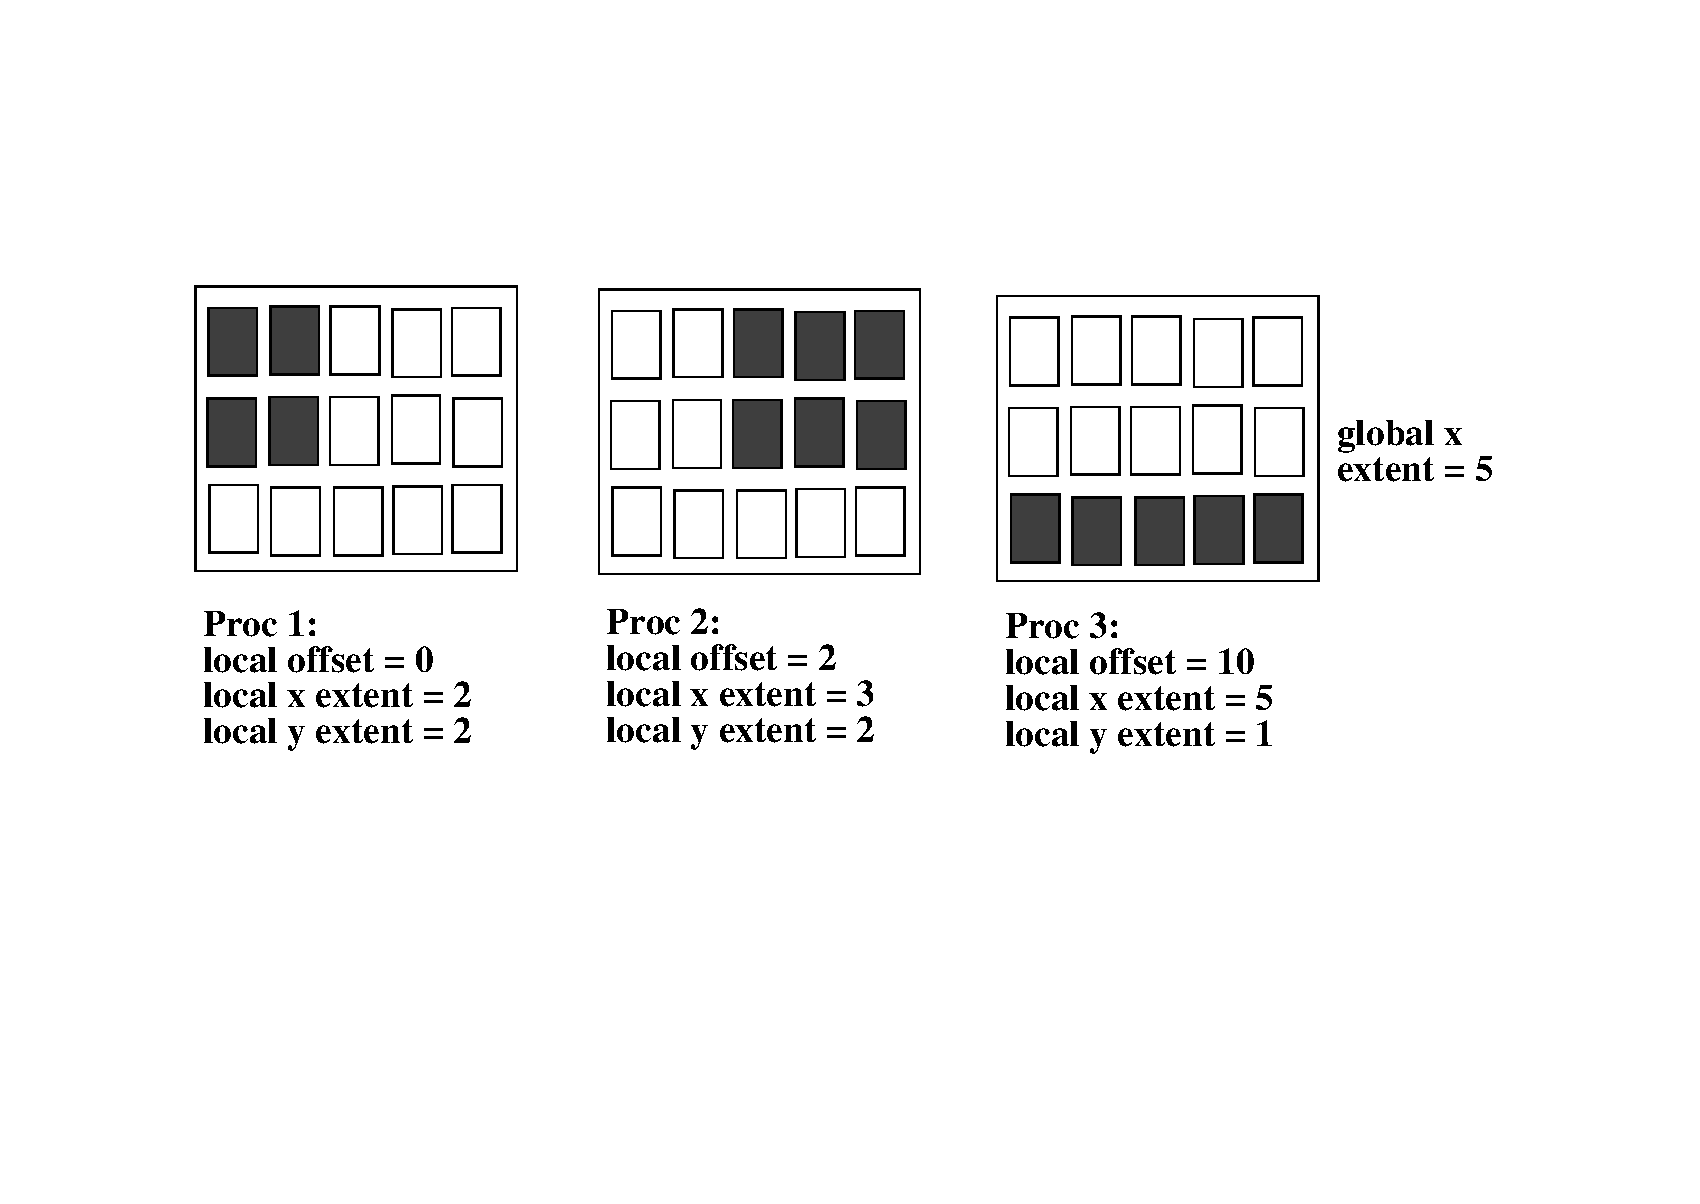
\includegraphics[scale=.6]{figures/box_new}
  \caption{Box partition. It is assumed here that the global index starts at 0
    in the upper left corner.}
  \label{box_partition}
\end{figure}
  
\subsubsection{Orange partition}

Each partition is an ensemble of segments in the global domain. Each
segment is described by its global offset and its local extent.  In
this case, we have {\tt ig\_paral(1:N)} where {\tt N = 2 + 2*number of
  segments}
% \footnote{As for the Box partition, the maximum number of segments
%   is presently 338; it can be increased by modifying the value of
%   {\tt Clim\_MaxSegments}}.

\begin{itemize}
\item {\tt ig\_paral(1)} = 3 (indicates a Orange partition)
\item {\tt ig\_paral(2)} = the total number of segments for the
  partition (limited to 200 presently, see note for ig\_paral(4) for
  Box partition above)
\item {\tt ig\_paral(3)} = the first segment global offset
\item {\tt ig\_paral(4)} = the first segment local extent
\item {\tt ig\_paral(5)} = the second segment global offset
\item {\tt ig\_paral(6)} = the second segment local extent
\item ...
\item {\tt ig\_paral(N-1)} = the last segment global offset
\item {\tt ig\_paral(N)} = the last segment local extent
\end{itemize}

Figure \ref{orange_partition} illustrates an Orange partition with 3
segments for one process. The other process partitions are not
illustrated.

\begin{figure}
  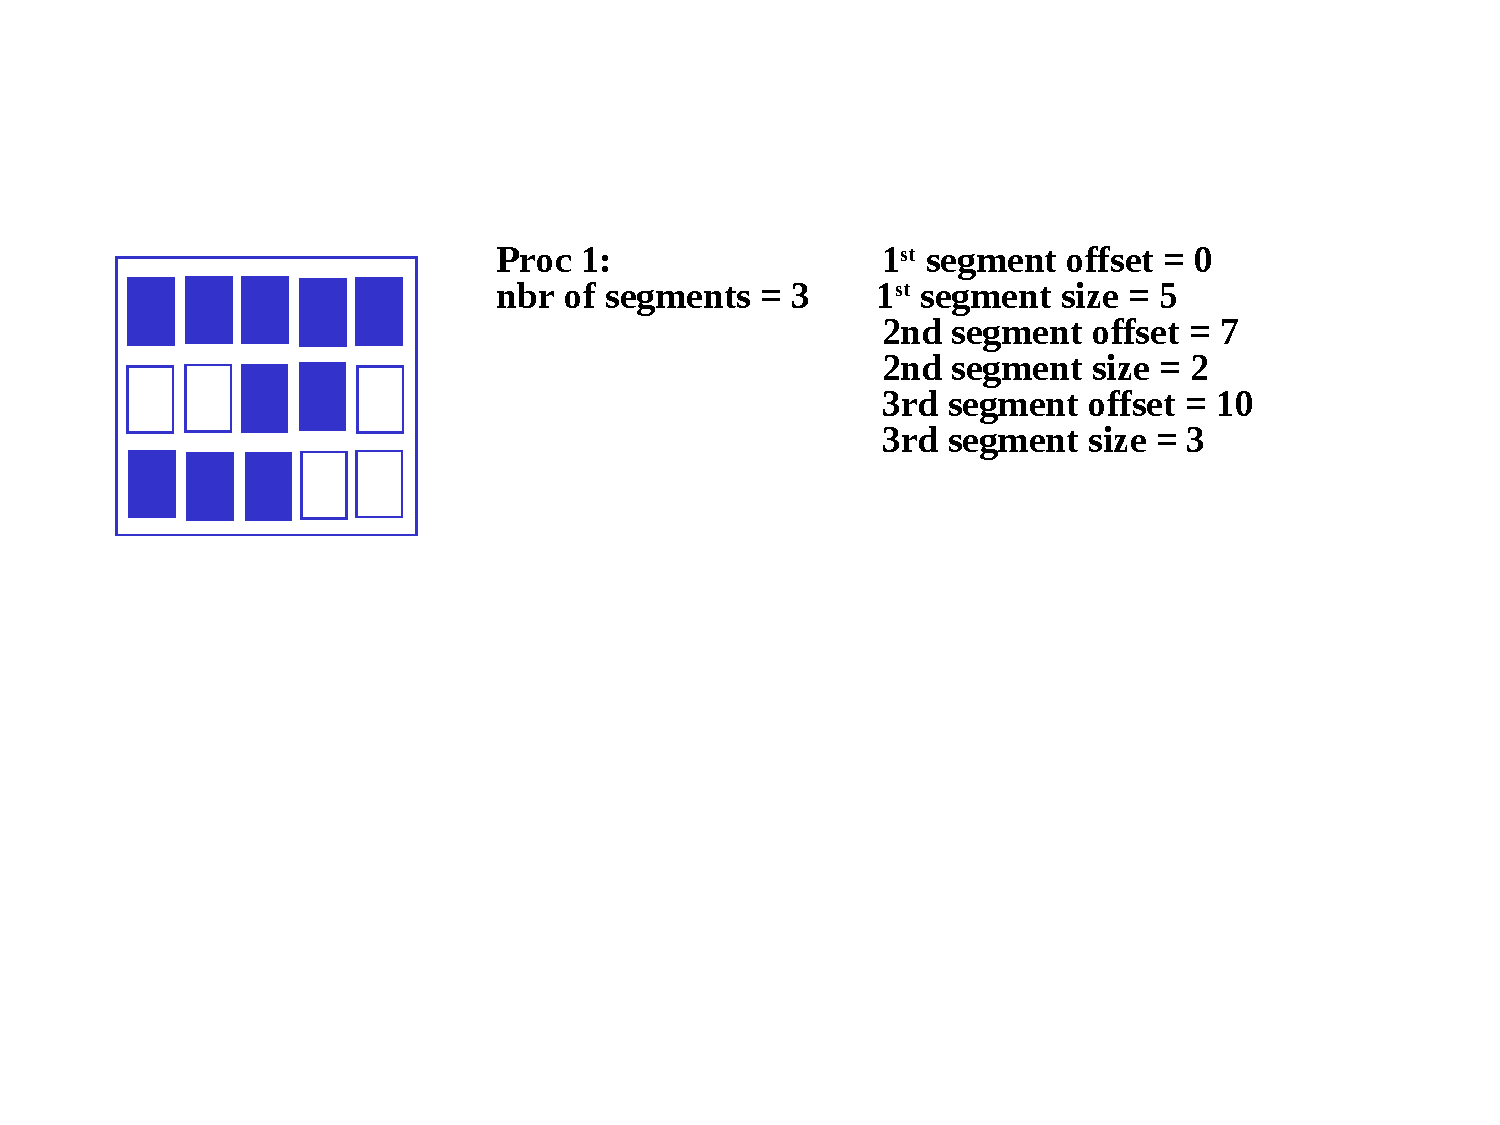
\includegraphics[scale=.6]{figures/orange_new}
  \caption{Orange partition for one process. It is assumed here that
    the global index starts at 0 in the upper left corner.}
  \label{orange_partition}
\end{figure}

\subsubsection{Points partition}
\label{subsubsec_pointspart}

This partition is a list of global indices associated with each
process.  The index naming
is arbitrary but must be consistent between all processes involved
in the partition description.  In
this case, we have {\tt ig\_paral(1:N)} where {\tt N = 2 + number of
  points}
% \footnote{As for the Box partition, the maximum number of segments
%   is presently 338; it can be increased by modifying the value of
%   {\tt Clim\_MaxSegments}}.

\begin{itemize}
\item {\tt ig\_paral(1)} = 4 (indicates a Points partition)
\item {\tt ig\_paral(2)} = number of points in the partition 
\item {\tt ig\_paral(3)} = the first global index
\item {\tt ig\_paral(4)} = the second global index
\item ...
\item {\tt ig\_paral(N)} = the last global index
\end{itemize}

% {Partition definition}
\subsection{Grid data file definition}
\label{subsubsec_griddef}

Grid data files (see section \ref{subsec_griddata}) are required by OASIS3-MCT for specific operations , i.e.  {\em grids.nc} and {\em masks.nc} for
{\tt SCRIPR} (see section \ref{subsec_interp}), and {\em masks.nc} and
{\em areas.nc} for {\tt CONSERV} (see section
\ref{subsec_cooking}). These grid data files can be created by the
user before the run or can be written directly at run time by the components with the following routines.
If a grid data files does not exist, the corresponding routine will create it; if the grid data file exists, the routine can be used to {\bf add} grid definition fields but it will not {\bf overwrite} grid definition fields already existing in the file with the same grid name. 

These routines can be called only by one component process to write the whole grid or by each process holding a part of a grid. In the former case, optional argument {\tt il\_part\_id} is not needed and the arrays (see below) handling the longitudes of the grid points or corners ({\tt lon}, {\tt clon}), the latitudes of the grid points or corners ({\tt lat}, {\tt clat}), the masks ({\tt mask}), fracs ({\tt frac}), and areas ({\tt area}) of the grid cells need to cover the whole grid; in the later case, the {\tt il\_part\_id} returned by {\tt oasis\_def\_partition} needs to be provided as input argument and the arrays need to cover only the local partition of the grid.

The field names in the {\em grids.nc}, {\em masks.nc}, and {\em areas.nc} follow a well-defined convention.  The fields are normally 2-dimensional, and each field name consists of the gridname followed by a string that identifies the field.  For instance, the center latitudes for the grid torc will be called torc.lat and the center longitudes will be called torc.lon in the netcdf file.  The {\em grids.nc} file contains the center latitudes (.lat) and longitudes (.lat) as well as the corner latitudes (.cla) and corner longitudes (.clo).  The corner fields have a third dimension associated with the number of corners per gridcell.  The {\em area.nc} file constains the area field (.srf).  The {\em masks.nc} file contains the mask (.msk) and frac (.frc) fields.

\begin{itemize}

\item {\tt CALL oasis\_start\_grids\_writing (flag)} or
\item {\tt CALL prism\_start\_grids\_writing (flag)}
  \begin{itemize}
  \item {\tt flag [INTEGER; OUT]}: always 1 
  \end{itemize} 
Must be called to start the grid writing process. 
  
  \vspace{0.2cm}
\item {\tt CALL oasis\_write\_grid (cgrid, nx\_global, ny\_global, lon, lat, il\_part\_id)}
\item {\tt CALL prism\_write\_grid (cgrid, nx\_global, ny\_global, lon, lat, il\_part\_id)}
        
  \begin{itemize}
  \item {\tt cgrid [CHARACTER; IN]}: grid name prefix (see
    \ref{subsec_namcouplesecond} and \ref{subsec_griddata}); maximum length of 64 characters (4 are usually used for historical reasons)
  \item {\tt nx\_global [INTEGER; IN]} : first dimension of the global grid 
  \item {\tt ny\_global [INTEGER; IN]} : second dimension of the global grid ({\tt =1} if the grid is expressed as a 1D vector) 
  \item {\tt lon [REAL, DIMENSION(nx,ny); IN]} : single or double real array of longitudes covering the whole grid ({\tt nx=nx\_global}, {\tt ny=ny\_global}) or only the local partition (degrees East).
  \item {\tt lat [REAL, DIMENSION(nx,ny); IN]} : single or double real array of latitudes covering the whole grid ({\tt nx=nx\_global}, {\tt ny=ny\_global}) or only the local partition (degrees North)
\item  {\tt il\_part\_id [INTEGER, OPTIONAL; IN]}: partition ID returned by {\tt oasis\_def\_partition}, see \ref{subsubsec_Partition}; needed if each component task holding a part of a decomposed grid writes its own part of the grid.
  \end{itemize}

  Writes the component grid longitudes and latitudes. Longitudes must be
  given in degrees East in the interval -360.0 to 720.0. Latitudes
  must be given in degrees North in the interval -90.0 to 90.0. Note
  that if some grid points overlap, it is recommended to define those
  points with the same number (e.g. 90.0 for both, not 450.0 for one
  and 90.0 for the other) to ensure automatic detection of overlap by
  OASIS3-MCT (which is essential to have a correct conservative
  remapping \texttt{SCRIPR/CONSERV}, see section \ref{subsec_interp}).

  \vspace{0.2cm}
\item {\tt CALL oasis\_write\_corner (cgrid, nx\_global, ny\_global, nc, clon, clat, il\_part\_id))}
\item {\tt CALL prism\_write\_corner (cgrid, nx\_global, ny\_global, nc, clon, clat, il\_part\_id))}

  \begin{itemize}
  \item {\tt cgrid }, {\tt nx\_global }, {\tt ny\_global }, {\tt il\_part\_id }: as for {\tt oasis\_write\_grid}

  \item {\tt nc [INTEGER; IN]} : number of corners per grid cell (can be any number)
  \item {\tt clon [REAL, DIMENSION (nx,ny,nc);IN]} : single or double real array of corner
    longitudes covering the whole grid ({\tt nx=nx\_global}, {\tt ny=ny\_global}) or only the local partition (in degrees\_East)
  \item {\tt clat [REAL, DIMENSION (nx,ny,nc);IN]} : single or double real array of corner
    latitudes covering the whole grid ({\tt nx=nx\_global}, {\tt ny=ny\_global}) or only the local partition (in degrees\_North)
  \end{itemize}

  Writes the grid cell corner longitudes and latitudes
  (counterclockwise sense). Longitudes must be given in degrees East
  in the interval -360.0 to 720.0. Latitudes must be given in degrees
  North in the interval -90.0 to 90.0. Note also that cells larger
  than 180.0 degrees in longitude are not supported. Writing of
  corners is optional as corner information is needed only for {\tt
    SCRIPR/CONSERV} (see section \ref{subsec_interp}). If called,
  needs to be called after {\tt oasis/prism\_write\_grid}.

  \vspace{0.2cm}
\item {\tt CALL oasis\_write\_mask (cgrid, nx\_global, ny\_global, mask, il\_part\_id, companion)}
\item {\tt CALL prism\_write\_mask (cgrid, nx\_global, ny\_global, mask, il\_part\_id, companion)}

  \begin{itemize}
  \item {\tt cgrid }, {\tt nx\_global }, {\tt ny\_global }, {\tt il\_part\_id }: as for {\tt oasis\_write\_grid}
  \item {\tt mask [INTEGER, DIMENSION(nx,ny) ;IN]} : mask array covering the whole grid ({\tt nx=nx\_global}, {\tt ny=ny\_global}) or only the local partition. Be careful about the OASIS historical convention (!): 0 = not masked (active), 1 = masked (not active).
  \item {\tt companion [CHARACTER ;IN; OPTIONAL]} : the character string value associated with the mask field attribute ``coherent\_with\_grid''.  This will be written to the {\em masks.nc} netcdf file with the mask field.  It is purely informational and used in cases where the mask field is derived from or consistent with another grid.
  \end{itemize}
  Writes the component grid mask.  The mask field should be consistent with the frac field and will define the 0/1 mask of the grid cell.  The mask field is used by both the {\tt SCRIPR} map generation function and in the {\tt CONSERV} operations if defined.  The mask field is written to the {\em masks.nc} file.

  \vspace{0.2cm}
\item {\tt CALL oasis\_write\_frac (cgrid, nx\_global, ny\_global, frac, il\_part\_id, companion)}
\item {\tt CALL prism\_write\_frac (cgrid, nx\_global, ny\_global, frac, il\_part\_id, companion)}

  \begin{itemize}
  \item {\tt cgrid }, {\tt nx\_global }, {\tt ny\_global }, {\tt il\_part\_id }: as for {\tt oasis\_write\_grid}
  \item {\tt frac [REAL, DIMENSION(nx,ny) ;IN]} : single or double real frac array covering the whole grid ({\tt nx=nx\_global}, {\tt ny=ny\_global}) or only the local partition.  
  \item {\tt companion [CHARACTER ;IN; OPTIONAL]} : the character string value associated with the frac field attribute ``coherent\_with\_grid''.  This will be written to the {\em masks.nc} netcdf file with the fraction field.  It is purely informational and used in cases where the frac field is derived from or consistent with another grid.
  \end{itemize}
  Writes the component grid cell fractions.  This should be consistent with the mask field and defines the fraction of the grid cell that is active (i.e. not masked).  The fraction field is only used in the {\tt CONSERV} operations. Either the mask or fractions must be defined for that operation.  If both are defined, they must be consistent; OASIS3-MCT will abort if they are not coherent or if both are missing.  Note that by OASIS conventions for the mask, a gridcell with mask=0 (active) should have a fractions greater than 0 and a gridcell with mask=1 (inactive) should have a fractions equal to 0.  The fraction field is written to the {\em masks.nc} file.

  \vspace{0.2cm}
\item {\tt CALL oasis\_write\_area (cgrid, nx\_global, ny\_global, area, il\_part\_id)}
\item {\tt CALL prism\_write\_area (cgrid, nx\_global, ny\_global, area, il\_part\_id)}

  \begin{itemize}
  \item {\tt cgrid }, {\tt nx\_global }, {\tt ny\_global }, {\tt il\_part\_id }: as for {\tt oasis\_write\_grid}
  \item {\tt area [REAL, DIMENSION(nx,ny); IN]} : single or double real array of grid cell
    areas covering the whole grid ({\tt nx=nx\_global}, {\tt ny=ny\_global}) or only the local partition 
  \end{itemize}
  Writes of the component grid cell areas. Needed for some {\tt SCRIPR} options and for the {\tt CONSERV}
  operation (see section \ref{subsec_cooking}).    The area field is written to the {\em areas.nc} file.
  The surfaces may be given in any units but they must be the same on the source and target sides; furthermore they must be in square radians if the True Area (TR) correction is activated, see section 4.3.

  \vspace{0.2cm}
\item {\tt CALL oasis\_write\_angle (cgrid, nx\_global, ny\_global, angle, il\_part\_id)}
\item {\tt CALL prism\_write\_angle (cgrid, nx\_global, ny\_global, angle, il\_part\_id)}

  \begin{itemize}
  \item {\tt cgrid }, {\tt nx\_global }, {\tt ny\_global }, {\tt il\_part\_id }: as for {\tt oasis\_write\_grid}
  \item {\tt angle [REAL, DIMENSION(nx,ny); IN]} : single or double real array of grid cell
    angles covering the whole grid ({\tt nx=nx\_global}, {\tt ny=ny\_global}) or only the local partition 
  \end{itemize}
  Writes of the component grid cell angles.  The angle field is written to the {\em grids.nc} file.  This field does not play a role in OASIS3-MCT implementation and is never needed.


  \vspace{0.2cm}
\item {\tt CALL prism\_terminate\_grids\_writing()} or
\item {\tt CALL oasis\_terminate\_grids\_writing()}

\end{itemize}

The creation of the different grid data files is completed in the routine
oasis\_enddef.

\subsection{Coupling field declaration}
\label{subsubsec_Declaration}

All processes of a component that send or receive a coupling field, or a part of it, needs to declare the coupling field.
 
Processes not implied in the
coupling do not have to call this routine at all (for backward
compatibility with OASIS3-MCT\_2.0, they may still call it with any {\tt name} and {\tt il\_part\_id}).

\begin{itemize}

\item {\tt CALL oasis\_def\_var (var\_id, name, il\_part\_id,
    var\_nodims, kinout, \newline var\_type,
    kinfo)} or
    
\item {\tt CALL oasis\_def\_var (var\_id, name, il\_part\_id,
    var\_nodims, kinout, \newline var\_actual\_shape, var\_type,
    kinfo)} or

\item {\tt CALL prism\_def\_var\_proto(var\_id, name, il\_part\_id,
    var\_nodims, kinout, var\_type, kinfo)} or

\item {\tt CALL prism\_def\_var\_proto(var\_id, name, il\_part\_id,
    var\_nodims, kinout, var\_actual\_shape, var\_type, kinfo)}

  \begin{itemize}
  \item {\tt var\_id [INTEGER; OUT]}: coupling field ID.  Note that all 
      coupling fields appearing in the {\it namcouple} must be defined with 
      a call to {\tt oasis\_def\_var}; not doing so would lead to an abort.  
      But all fields defined with a call to {\tt oasis\_def\_var} must not necessarily 
      appear in the {\it namcouple}. If a field does not appear in the {\it namcouple}, 
      the {\tt var\_id} returned by the {\tt oasis\_def\_var} will be equal to -1; 
      the value of the {\tt var\_id} should be tested and the corresponding 
      {\tt oasis\_put} and {\tt oasis\_get} should not be called if {\tt var\_id} 
      equals -1. These constraints are imposed to avoid that a typo in the {\it namcouple}
       would lead to coupling exchanges not corresponding to what the user intends to activate. 
  \item {\tt name [CHARACTER; IN]}: field symbolic name (as in the
    {\it namcouple}); maximum length of 80 characters
  \item {\tt il\_part\_id [INTEGER; IN]}: partition ID returned from {\tt oasis\_def\_partition} (see section
    \ref{subsubsec_Partition})
  \item {\tt var\_nodims [INTEGER, DIMENSION(2); IN]}: is an integer array of size two.  
    The first element, var\_nodims(1), is not used anymore in OASIS3-MCT, so 
    its value can be anything; The second element, var\_nodims(2),
    is the number of fields in a bundle (this will be 1 for unbundled
    fields or greater than 1 for fields that are bundled; note that
    if var\_nodims(2)=0, it will be automatically reset to 1 in the
    routine, to ensure backward compatibility).
  \item {\tt kinout [INTEGER; IN]}: {\tt OASIS\_In} or {\tt PRISM\_In}
    (i.e. = 21) for fields received by the component; {\tt OASIS\_Out},
    {\tt PRISM\_Out} (i.e. = 20) for fields sent by the component
    \footnote{Parameters OASIS\_In, PRISM\_In, OASIS\_Out, PRISM\_Out
      are defined in
      oasis3-mct/lib/psmile/src/mod\_oasis\_parameters.F90}.
  \item {\tt var\_actual\_shape [INTEGER, DIMENSION(2*id\_var\_nodims(1)), IN]}:
    is not used anymore.  The interface has recently
    been overloaded, and this argument is no longer required.  But 
    for backwards compatibility, it can still be passed; if so, it has to be a vector of integers of any length (for simplicity we advise to pass a vector of length 1).
  \item {\tt var\_type [INTEGER; IN]}: type of coupling field array;
    put {\tt OASIS\_Real} or {\tt PRISM\_Real} (i.e. = 4) for single
    or double precision real arrays.  All coupling data is treated as
    double precision in the coupling layer, but conversion to or from
    single precision data is supported in the interface.
  \item {\tt kinfo [INTEGER; OUT]}: returned error code.
  \end{itemize}
\end{itemize}
% {coupling field declaration}

\subsection{End of definition phase}
\label{subsubsec_Endofdefinition}
All processes of components at least partly involved in the coupling (e.g. {\tt comp3} in figure
    \ref{Fig_coupling_layouts_b}) have to close the definition phase. Different configurations of components and corresponding use of {\tt oasis\_enddef} are described in section \ref{sec_deploy} and on figures \ref{Fig_coupling_layouts_a} and \ref{Fig_coupling_layouts_b}.
\begin{itemize}
\item {\tt CALL oasis\_enddef (kinfo)}
\item {\tt CALL prism\_enddef\_proto(kinfo)}
  \begin{itemize}
  \item kinfo [INTEGER; OUT]: returned error code.
  \end{itemize}
\end{itemize}

% {End of definition phase}

\subsection{Sending ``put'' and receiving ``get'' actions}
\label{subsubsec_sendingreceiving}

This section describes how to send (put) and receive (get) fields through
the coupling interface.  This interface supports several ranks and
types of coupling fields.  First, the fields passed into the interface can be 
4 byte or 8 byte reals. The field decomposition must be 
consistent with the decomposition defined in the grid partition (see \ref{subsubsec_Partition})\footnote{But the decomposition of each field can be either one
dimensional or two dimensional and does not
have to match the rank of the grid partition.}  Third, the fields
can be bundled, i.e. have an extra (non-spatial) dimension like for a field covering different ice categories.  The bundled dimension is always the last dimension in any
field passed into the get and put routines.  And the size of the bundle dimension
must match the value defined for the variable in var\_nodims(2) in the
{\tt oasis\_def\_var} interface (see section \ref{subsubsec_Declaration}).

So in general, the fields passed into the get and put interface can have rank
1, 2, or 3 and include the following possible options where fld can be a 4
byte or 8 byte real array.

\begin{itemize}
\item 1D, fld(:) = an single, unbundled field of decomposition rank 1.
\item 2D, fld(:,:) = a single, unbundled field of decomposition rank 2.
\item 1D bundled, fld(:,:) = a bundled set of fields of decomposition rank 1.
  The size of the second dimension must equal the number of fields in the 
  bundle, defined by var\_nodims(2) in the {\tt oasis\_def\_var} interface.
\item 2D bundled, fld(:,:,:) = a bundled set of fields of decomposition rank 2.
  The size of the third dimension must equal the number of fields in the 
  bundle, defined by var\_nodims(2) in the {\tt oasis\_def\_var} interface.
\end{itemize}

%With bundled fields, it is important that the number of fields in the bundle match
%in the two models being coupled.  This requires that the var\_nodims(2) values
%in the send and receive model match the bundle dimension of that bundled coupling field.
Different bundled fields
can have different numbers of fields, but for a given bundled field, the
number of fields must match on the send and receive side.  This is explicitly
checked within the coupling layer and will lead to an abort if not done correctly.
It is possible to define a 1D bundled or 2D bundled field  with a bundle dimension of 1, i.e. for a bundle that contains only one single field.

Finally, the bundled field option can be used to
bundle together multi-level variables, multiple related fields, and other types
of fields.  The fields must share a common partition and common namcouple settings (e.g. interpolation)
to be bundled.  While this is a useful feature for multi-level fields, {\bf this does not mean
that 3D interpolation is supported}.
Each field in the bundle is
treated internally as a separate field in the coupling layer without
any information about the relationship between the fields in the bundle.  In fact,
the bundled field variables are internally renamed and a field number is appended
to the variable name to keep track of the distinct fields in the bundle.  That
updated variable name will appear in restart and output files.


\subsubsection{Sending a coupling (or I/O) field or writing a coupling restart file}
\label{prismput}

In the component time step loop, each process sends its part of the
coupling (or I/O) field.

\begin{itemize}
\item {\tt CALL oasis\_put (var\_id, date, fld1, info, fld2, fld3,
    fld4, fld5, write\_restart)}
\item {\tt CALL prism\_put\_proto(var\_id, date, fld1, info, fld2,
    fld3, fld4, fld5, write\_restart)}
  \begin{itemize}
  \item {\tt var\_id [INTEGER; IN]}: field ID (returned from corresponding {\tt
      oasis\_def\_var}, see section \ref{subsubsec_Declaration})
  \item {\tt date [INTEGER; IN]}: number of seconds (or any other time
    units as long as the same are used in all components and in the {\it
      namcouple}) at the time of the call (by convention at the
    beginning of the timestep)
  \item {\tt fld1 [REAL, IN]}: coupling (or I/O) field array; can be
    1D, 2D, bundled 1D, or bundled 2D, see baove. 
  \item {\tt info [INTEGER; OUT]}: returned info code:
    \begin{itemize}
    \item {\tt OASIS\_Sent} (=4) if the field was sent to another component
    \item {\tt OASIS\_LocTrans} (=5) if the field was only used in a time
      transformation (not sent, not output)
    \item {\tt OASIS\_ToRest} (=6) if the field was written to a restart
      file only
    \item {\tt OASIS\_Output} (=7) if the field was written to an output
      file only
    \item {\tt OASIS\_SentOut} (=8) if the field was both written to an
      output file and sent to another component 
    \item {\tt OASIS\_ToRestOut} (=9) if the field was written both to a
      restart file and to an output file.
    \item {\tt OASIS\_WaitGroup} (=14) if the field was not sent because it is part of a group.
    It will be sent only when the {\tt oasis\_put} of the last field in the group will be called; however, the field is buffered and therefore the field array can be modified in the component code when returning from the oasis\_put call.
    \item {\tt OASIS\_Ok} (=0) otherwise and no error occurred.
    \end{itemize}
  \item {\tt fld2 [REAL, IN, OPTIONAL]}: optional $2^{nd}$ coupling
    field array; can be 1D, 2D, bundled 1D, or bundled 2D.  Rank and size
    must match {\tt fld1}.
  \item {\tt fld3 [REAL, IN, OPTIONAL]}: optional $3^{rd}$ coupling
    field array; can be 1D, 2D, bundled 1D, or bundled 2D.  Rank and size
    must match {\tt fld1}.
  \item {\tt fld4 [REAL, IN, OPTIONAL]}: optional $4^{th}$ coupling
    field array; can be 1D, 2D, bundled 1D, or bundled 2D.  Rank and size
    must match {\tt fld1}.
  \item {\tt fld5 [REAL, IN, OPTIONAL]}: optional $5^{th}$ coupling
    field array; can be 1D, 2D, bundled 1D, or bundled 2D.  Rank and size
    must match {\tt fld1}.
  \item {\tt write\_restart [LOGICAL, IN, OPTIONAL]}: optional argument to write an 
    intermediate restart file associated with the variable {\tt
      var\_id} at the current timestep (see below).
  \end{itemize}
\end{itemize}

To ensure a proper use of the {\tt oasis\_put}, one has to take care
of the following aspects:

\begin{itemize}

\item A $2^{nd}$, $3^{rd}$, $4^{th}$ and $5^{th}$ source field can be
  passed as optional arguments. If so, the $2^{nd}$, $3^{rd}$,
  $4^{th}$ and $5^{th}$ set of weights present in the remapping file
  will be applied, respectively (see section \ref{subsec_mapdata} for
  the remapping file format). This will be used for example for the {\tt
    SCRIPR/BICUBIC} remapping for which a $1^{st}$, $2^{nd}$,
  $3^{rd}$, $4^{th}$ set of weights should be respectively applied to
  the field value, its gradient in the first dimension, its gradient
  in the second dimension, and its cross-gradient in that order. 

  This will be used also for the CONSERV/SECOND for which a 1st, 2nd, 3rd 
  set of weights should be respectively applied to the field value, its 
  gradient with respect to the latitude ($\theta$) $\frac{\delta f}{\delta \theta}$
  and its gradient with respect to the longitude ($\phi$) $\frac{1}{cos \theta}\frac{\delta f}{\delta \phi}$ 
  in that order.

  Bicubic and higher order
  remapping are therefore supported given that the higher order fields
  are provided at each time step as {\tt oasis\_put} arguments. Note
  that if {\tt fld3}, or {\tt fld4}, or {\tt fld5} are passed, {\tt fld2}, or {\tt fld3} and 
  {\tt fld2}, or {\tt fld4} and {\tt fld3} and {\tt fld2} must also be passed respectively.
  
\item {\bf Note that from OASIS3-MCT\_4.0 onwards, 
the number of weights in the remapping file and the number of fields in the coupling restart file 
(when such a file is needed) must strictly match the number of source fields passed to the 
oasis\_put .}

%\item Trying to send with {\tt oasis\_put} a field declared with a
%  {\tt oasis\_def\_var} but not defined in the configuration file {\it
%    namcouple} will lead to an abort. In this case, the field ID
%  returned by the {\tt oasis\_def\_var} is equal to -1 and the
%  corresponding {\tt oasis\_put} should not be called.

\item This routine may be called by the component at each timestep. The
  convention for the {\tt date} argument is to indicate the time at
  the beginning of the timestep. The sending is actually performed
  if the time obtained by adding the field lag ({\tt LAG} in the
  {\em namcouple}, if any, with {\tt LAG=0} by default) to the {\tt date} corresponds to a time at which it
  should be activated, given the coupling or I/O period indicated by
  the user in the {\it namcouple} (see section \ref{sec_namcouple}).

\item By convention, the first coupling
  of a run occurs at {\tt date=0} and the final coupling occurs
  at {\tt date = runtime-cpl\_period}, where {\tt runtime} is the total time of
  the run and {\tt cpl\_period} is the coupling period of the field indicated by
  the user in the {\it namcouple} (see section \ref{sec_namcouple}).

\item For a coupling
  field with a positive lag, the coupling restart file (see section
  \ref{subsec_restartdata}) is automatically overwritten by the {\tt
    oasis\_put} when the {\tt date+LAG=runtime}.

  % \item A field will not be sent at all if its coupling (or I/O)
  %   period indicated in the {\it namcouple} is greater than the
  %   total run time.

\item The total run time should match an integer number of coupling
  periods.

\item If a local time transformation is indicated for the field by the
  user in the {\it namcouple} (INSTANT, AVERAGE, ACCUMUL, T\_MIN or
  T\_MAX, see section \ref{sec_transformations}), it is automatically
  performed and the resulting field is finally sent at the coupling or
  I/O frequency.  For non-instant transformations, partially
  transformed fields will be written to the restart file at the end of
  the run for use on the next component startup, when needed.

\item A coupling field sent by a source component can be
  associated with more than one target field and component, if specified
  as so with different entries in the {\it namcouple} configuration
  file. In that case, the source component needs to send the field only
  once and the corresponding data will arrive at multiple targets as
  specified in the {\it namcouple}. Different coupling frequencies and
  transformations are allowed for different coupling exchanges of the
  same field. If coupling restart files are required (either if a {\tt
    LAG} or if a {\tt LOCTRANS} transformation is specified), it is
  mandatory to specify different files for the different fields.

\item Trying to send with {\tt oasis\_put} a field declared with a {\tt
  oasis\_def\_var} but not defined in the configuration file {\it
  namcouple} will lead to an abort. When a field is not defined in the {\it namcouple}, the field ID
returned by the {\tt oasis\_def\_var} is equal to -1 and the
corresponding {\tt oasis\_put} should not be called. 

\item Support to couple multiple fields via a single communication.
This is supported through colon delimited field lists in the namcouple (see \ref{subsubsec_secondEXPORTED}). 
All fields will use the namcouple settings for that entry. In the component
model codes, these fields are still sent ({\bf “put”}) one at a time. Inside
OASIS3-MCT, the fields are stored and a single mapping and send instruction is executed
for all fields. This is useful in cases where multiple fields have the same coupling transformations
and to reduce communication costs by aggregating multiple fields into a single communication.

This option does not put any constraint
on the order of the related {\tt oasis\_put} and {\tt oasis\_get} in the codes.

As they appear in one single entry line, these fields must share the same coupling restart file 
but this restart file may contain other fields.

\item The optional argument, {\tt write\_restart}, in the {\tt oasis\_put} routine is {\bf false} by default. 
If a user sets that argument to true, a restart file will be written for that field {\bf only for that timestep}. The {\tt write\_restart} 
will just save the data that exists at the time of the call, taking into account lags and LOCTRANS operations. In 
cases where multiple fields are coupled as a single operation in the model (indicated via a list of colon delimited 
fields in the {\it namcouple}, see \ref{subsubsec_secondEXPORTED}), users are encouraged to specify 
the {\tt write\_restart} flag on ALL {\tt oasis\_put} calls at a given
time for this set of fields.
Intermediate restarts will be created with a timestamp prepended to
their filename, like TA000003600\_rst4.nc or TC000014400\_rst4.nc. 
A restart file that starts with TA will be a restart file associated
with LOCTRANS operations. A restart 
file that starts with TC will be a restart file associated with
coupling operations. The 9 digit timestamp in 
the filename is the date in seconds at the time of the oasis\_put
call. The restart filename (ie. rst4.nc) 
defined in the namcouple for variables will be used to generate a filename for intermediate restart files.
\end{itemize}

\subsubsection{Receiving a coupling (or I/O) field}

In the component time stepping loop, each process receives its part of the
coupling field.

\begin{itemize}
 
\item {\tt CALL oasis\_get (var\_id, date, fld, info)}
\item {\tt CALL prism\_get\_proto(var\_id, date, fld, info)}
  \begin{itemize}
  \item {\tt var\_id [INTEGER; IN]}: field ID (returned by the corresponding
    {\tt oasis\_def\_var})
  \item {\tt date [INTEGER; IN]}: number of seconds (or any other time
    units as long as the same are used in all components and in the {\it
      namcouple}) at the time of the call (by convention at the
    beginning of the timestep)
  \item {\tt fld [REAL, OUT]}: I/O or coupling field array;  
    can be 1D, 2D, bundled 1D, or bundled 2D.
  \item {\tt info [INTEGER; OUT]}: returned info code:
    \begin{itemize}
    \item OASIS\_Recvd(=3) if the field was received from another
      component
    \item OASIS\_FromRest (=10) if the field was read from a restart
      file only
    \item OASIS\_Input (=11) if the field was read from an input file
      only
    \item OASIS\_RecvOut (=12) if the field was both received from
      another component and written to an output file
    \item OASIS\_FromRestOut (=13) if the field was both read from a
      restart file and written to an output file
    \item OASIS\_Ok (=0) otherwise and no error occurred.
    \end{itemize}
  \end{itemize}
\end{itemize}

To ensure a proper use of the {\tt oasis\_get}, one has to take care of the following aspects:

\begin{itemize}

\item This routine may be called by the component at each timestep. The {\tt
  date} argument is automatically analysed and the receiving action is
actually performed only if {\tt date} corresponds to a time for which
it should be activated, given the period indicated by the user in the
{\it namcouple}. An exchange at the beginning of the run at time=0 is
expected.

\item Trying to receive with {\tt oasis\_get} a field declared with a {\tt
  oasis\_def\_var} but not defined in the configuration file {\it
  namcouple} will lead to an abort. In this case, the field ID
returned by the {\tt oasis\_def\_var} is equal to -1 and the
corresponding {\tt oasis\_get} should not be called. 

\item If a coupling field has a positive lag, the coupling field that
  matches the {\tt oasis\_get} at time=0 will come from a coupling
  restart file written by the last active {\tt oasis\_put} of the
  previous run (see section \ref{subsec_lag}). 

\item Support to couple multiple fields via a single communication.
This is supported through colon delimited field lists in the namcouple (see \ref{subsubsec_secondEXPORTED}). 
All fields will use the namcouple settings for that entry. In the component
model codes, these fields are still received (via an {\tt oasis\_get}) one at a time. Inside
OASIS3-MCT, the fields are stored and a single mapping and receive instruction is executed
for all fields. This is useful in cases where multiple fields have the same coupling transformations
and to reduce communication costs by aggregating multiple fields into a single communication. If a
LOCTRANS transformation is needed for these multiple fields, it is necessary to define a restart file
for these multiple fields.
\end{itemize}

\subsection{Termination}
\label{subsubsec_Termination}

\begin{itemize}

\item {\tt CALL oasis\_terminate (kinfo)}
\item {\tt CALL prism\_terminate\_proto(kinfo)}
  \begin{itemize}
  \item {\tt kinfo [INTEGER; OUT]}: returned error code.
  \end{itemize}
All processes of components at least partly involved in the coupling (e.g. {\tt comp3} in figure
    \ref{Fig_coupling_layouts_b}) have to terminate the coupling by
  calling this routine\footnote{If the process called {\tt MPI\_Init}
    (before calling {\tt oasis\_init\_comp}), it must also call {\tt
      MPI\_Finalize} explicitly, but only after calling {\tt
      oasis\_terminate\_proto}.}(normal termination). Different configurations of components and corresponding use of {\tt oasis\_terminate} are described in section \ref{sec_deploy} and on figures \ref{Fig_coupling_layouts_a} and \ref{Fig_coupling_layouts_b}.

  

\end{itemize}

% {Termination}

\subsection{Auxiliary routines}
\label{subsubsec_auxroutines}

The following auxiliary routines are currently available.

\begin{itemize}
\item {\tt CALL oasis\_abort (compid, routine\_name, abort\_message, file, line, rcode)}
\item {\tt CALL prism\_abort\_proto(compid, routine\_name,
    abort\_message, file, line, rcode)}
  \begin{itemize}
  \item {\tt compid [INTEGER; IN]}: component ID (from {\tt
      oasis\_init\_comp})
  \item {\tt routine\_name [CHARACTER*; IN]}: name of calling routine
  \item {\tt abort\_message [CHARACTER*; IN]}: message to be written out
  \item {\tt file [CHARACTER*; OPTIONAL; IN]}: file from which oasis\_abort is called from
  \item {\tt line [INTEGER, OPTIONAL; IN]}: line in file from which oasis\_abort is called from
  \item {\tt rcode [INTEGER, OPTIONAL; IN]}: Optional argument. When OASIS 
    aborts, it returns rcode if it is present, else it returns 1
  \end{itemize}

  If a process needs to abort voluntarily, it should do so by calling
  {\tt oasis\_abort}. This will ensure a proper termination of all
  processes in the coupled model communicator. This routine writes the
  name of the calling component, the name of the calling routine, and the
  message to the process debug file (see {\tt \$NLOGPRT} in section
  \ref{subsec_namcouplefirst}).  This routine cannot be called before
  {\tt oasis\_init\_comp}.

  \vspace{0.2cm}
\item {\tt CALL oasis\_get\_debug(debug, kinfo)}
\item {\tt CALL prism\_get\_debug(debug, kinfo)}
  \begin{itemize}
  \item {\tt debug [INTEGER; OUT]}: output debug value
  \item {\tt kinfo [INTEGER; OUT; OPTIONAL]}: returned error code
  \end{itemize}

  This routine may be called at any time to retrieve the current
  OASIS3-MCT internal debug level (see {\tt \$NLOGPRT} in section
  \ref{subsec_namcouplefirst}).  This is useful if the user wants to
  return the original debug value after changing it.

  \vspace{0.2cm}
\item {\tt CALL oasis\_set\_debug(debug, kinfo)}
\item {\tt CALL prism\_set\_debug(debug, kinfo)}
  \begin{itemize}
  \item {\tt debug [INTEGER; IN]}: input debug value
  \item {\tt kinfo [INTEGER; OUT; OPTIONAL]}: returned error code
  \end{itemize}

  This routine may be called at any time to change the debug level in
  OASIS3-MCT.  This method allows users to vary the debug level at
  different points in the component integration.

  \vspace{0.2cm}
\item {\tt CALL oasis\_get\_intercomm(new\_comm, cdnam, kinfo)}
\item {\tt CALL prism\_get\_intercomm(new\_comm, cdnam, kinfo)}
  \begin{itemize}
  \item {\tt new\_comm [INTEGER; OUT]}: MPI inter-communicator
  \item {\tt cdnam [CHARACTER*; IN]}: other component name (i.e. 2nd argument of  the call to {\tt oasis\_init\_comp} in that component)
  \item {\tt kinfo [INTEGER; OUT; OPTIONAL]}: returned error code
  \end{itemize}

  This routine sets up an MPI inter-communicator between two components,
  the local component and the component
  associated with {\tt cdnam}.  This call is collective across the
  tasks of the two components only.
  An MPI inter-communicator preserves the rank of the original communicators
  and does not allow collective communication within the communicator.  It
  provides point to point communication between two non-overlapping MPI groups.
  This method must be called synchronously across all components involved to
  minimize the chance of a deadlock, and it should be called only after
  {\tt oasis\_enddef} is called.
  See {\tt oasis\_get\_intracomm} below to create an intra-communicator.

  \vspace{0.2cm}
\item {\tt CALL oasis\_get\_intracomm(new\_comm, cdnam, kinfo)}
\item {\tt CALL prism\_get\_intracomm(new\_comm, cdnam, kinfo)}
  \begin{itemize}
  \item {\tt new\_comm [INTEGER; OUT]}: MPI intra-communicator
  \item {\tt cdnam [CHARACTER*; IN]}: other component name (i.e. 2nd argument of the call to {\tt oasis\_init\_comp} in that component).  This argument is a single string.
  \item {\tt kinfo [INTEGER; OUT; OPTIONAL]}: returned error code
  \end{itemize}

  This routine sets up an MPI intra-communicator between two 
  components, the local component and the component defined by
  the string {\tt cdnam}.  This call is collective
  across the tasks of the two components creating the intra-communicator only,
  and it must be called synchronously across all tasks of the two components
  to minimize the chance of a deadlock.  It should be called only after
  {\tt oasis\_enddef} is called.
  This method creates a new communicator consisting of a new collective group
  of tasks with new ranks.
  This communicator supports collective communications and is
  more typically used in MPI applications than inter-communicators
  (see {\tt oasis\_get\_intercomm} above).
  See also {\tt oasis\_get\_multi\_intracomm} for another method that
  supports creating an MPI intra-communicator between two or more components.

  \vspace{0.2cm}
\item {\tt CALL oasis\_get\_multi\_intracomm(new\_comm, cdnam, root\_ranks, kinfo)}
\item {\tt CALL prism\_get\_multi\_intracomm(new\_comm, cdnam, root\_ranks, kinfo)}
  \begin{itemize}
  \item {\tt new\_comm [INTEGER; OUT]}: MPI intra-communicator
  \item {\tt cdnam [CHARACTER*; IN]}: array of component names (i.e. 2nd argument of the call to {\tt oasis\_init\_comp} in that component).  This argument is a 1d array of character strings (i.e. cdnam(:)).
  \item {\tt root\_ranks [INTEGER; OUT]}: array of root ranks.  This argument is a 1d integer array (i.e. root\_ranks(:)) of the same size as {\tt cdnam}.
  \item {\tt kinfo [INTEGER; OUT]}: returned error code
  \end{itemize}

  This routine sets up an MPI intra-communicator between two or more
  components defined by the component names passed in the {\tt cdnam} array
  argument.  The local model name MUST BE one of the
  models defined in the {\tt cdnam} array.  The component names must 
  be valid names, but empty strings are allowed and ignored.
  This call is collective
  across all the tasks of the components defined in {\tt cdnam},
  and it must be called synchronously and consistently across all tasks of
  those components to minimize the chance of a deadlock.  It should be called only after
  {\tt oasis\_enddef} is called.
  This method creates a new communicator consisting of a new collective group
  of tasks with new ranks.  The root ranks of the individual components relative
  to the new communicator is output in the {\tt root\_ranks} argument.
  The size of {\tt cdnam} and {\tt root\_ranks} should be identical,
  and the values of {\tt root\_ranks} are consistent with the order of {\tt cdnam}..
  This communicator supports collective communications and is
  more typically used in MPI applications than inter-communicators
  (see {\tt oasis\_get\_intercomm} above).  
  See also {\tt oasis\_get\_intracomm} for another method that
  supports creating an MPI intra-communicator between two components.

\item {\tt CALL oasis\_put\_inquire(var\_id, date, kinfo)}
\item {\tt CALL prism\_put\_inquire\_proto(var\_id, date, kinfo)}
  \begin{itemize}
  \item {\tt var\_id [INTEGER; IN]}: field ID (from
  corresponding oasis\_def\_var)
  \item {\tt date [INTEGER; IN]}: as in {\tt oasis\_put}, number of seconds (or any other time
    units as long as the same are used in all components and in the {\it
      namcouple}) in the run at the time of the call
  \item {\tt kinfo [INTEGER; OUT]}: returned info code
    \begin{itemize}
    \item OASIS\_Sent(=4) if the field would be sent to another component
    \item OASIS\_LocTrans (=5) if the field would be only used in a time
      transformation (not sent, not output)
    \item OASIS\_ToRest (=6) if the field would be written to a restart
      file only
    \item OASIS\_Output (=7) if the field would be written to an output
      file only
    \item OASIS\_SentOut (=8) if the field would be both written to an
      output file and sent to another component (directly or via OASIS3
      main process)
    \item OASIS\_ToRestOut (=9) if the field would be written both to a
      restart file and to an output file.
    \item OASIS\_Ok (=0) otherwise and no error occurred.
    \end{itemize}
  \end{itemize}

This routine may be called at any time to
inquire what would happen to the corresponding field (i.e. with same
{\tt var\_id} and at same {\tt date}) below the corresponding {\tt
  oasis\_put}. This maybe useful if, for example, the calculation of
a coupling field is costly and if one wants to compute it only when it is
really sent out.

\item {\tt CALL oasis\_get\_ncpl(var\_id, ncpl, kinfo)}
\item {\tt CALL prism\_get\_ncpl\_proto(var\_id, ncpl, kinfo)}
  \begin{itemize}
  \item {\tt var\_id [INTEGER; IN]}: field ID (from
  corresponding oasis\_def\_var)
  \item {\tt ncpl [INTEGER; OUT]}: number of coupling exchanges in which the field
  is involved (i.e. when a field is sent to multiple targets) 
  \item {\tt kinfo [INTEGER; OUT]}: returned info code
  \end{itemize}

This routine returns the number of coupling exchanges in which the field var\_id is
involved. This number is needed to get the coupling frequencies with the
routine oasis\_get\_freqs, see below.

\item {\tt CALL oasis\_get\_freqs(var\_id, mop, ncpl, cpl\_freqs, kinfo)}
\item {\tt CALL prism\_get\_freqs\_proto(var\_id, mop, ncpl, cpl\_freqs, kinfo)}
  \begin{itemize}
  \item {\tt var\_id [INTEGER; IN]}: field ID (from
  corresponding oasis\_def\_var)
  \item {\tt mop [INTEGER; IN]}: OASIS\_Out or OASIS\_In type
  \item {\tt ncpl [INTEGER; IN]}: number of couplings in which the field
  is involved (i.e. when a field is sent to multiple targets)
   \item {\tt cpl\_freqs [INTEGER; DIMENSION(ncpl); OUT]}: coupling period(s) 
  (in number of seconds) of field var\_id. There is one coupling period for
  each coupling exchange in which the field is involved
  \item {\tt kinfo [INTEGER; OUT]}: returned info code
  \end{itemize}

This routine can be used to retrieve the coupling period(s) of field with
corresponding {\tt var\_id}, as defined in the {\it namcouple}

\end{itemize}

\section{OASIS3-MCT C API}
\label{APIC} 

OASIS3-MCT is distributed with C bindings and can be called from models written
in C and in C++.  These bindings leverage the Fortran ISO\_C\_BINDING standard.  
The C bindings can be compiled into static or shared libraries by the
OASIS3-MCT TopMakefileOasis3 as documented in \ref{subsec_compile}.

The C interfaces largely match
up with equivalent interfaces in Fortran.  An interface named
{\tt oasis\_interface} in Fortran can be expected to be named
{\tt oasis\_c\_interface} in C.

All of the C interfaces return an integer error code which can be
tested against the {\tt OASIS\_Ok} (or the equivalent {\tt
  OASIS\_Success}) constant.
The {\tt OASIS\_CHECK\_ERR} macro aborts
OASIS3-MCT with a meaningful message in the debug files in case of failure.
For most of the functions,
the return code is consistent with the {\tt
  kinfo} argument in the Fortran interfaces. However, for the put and get communication functions, the return error code only indicates
success or failure, while the detailed status is returned by the {\tt
  kinfo} argument (equivalent to the returned value of {\tt
  info} argument for the Fortran {\tt oasis\_put} and {\tt oasis\_get} routines, see section \ref{prismput}).
 
For example, the following constructs are equivalent in the two languages:

\begin{verbatim}
call oasis_get_localcomm(localcomm, kinfo)
if (kinfo .ne. OASIS_Ok)  &
   &  call OASIS_Abort(comp_id, "oasis_get_localcomm", &
   &  "Runtime error", __FILE__, __LINE__)
\end{verbatim}

and

\begin{verbatim}
OASIS_CHECK_ERR(oasis_get_localcomm(localcomm))
\end{verbatim}

For convenience a similar macro {\tt OASIS\_CHECK\_MPI\_ERR} has been
defined for testing the return code of any MPI function against {\tt
  MPI\_SUCCESS} and cleanly aborting OASIS3-MCT in case of failure.

\vspace{0.2cm}
More information about all these interfaces can be found in the
Fortran interface section (see \ref{API}). Use of these C bindings are illustrated in practical examples in
directories {\tt /C} in the different subdirectories in {\tt pyoasis/examples/}. Notes and deviations from
the Fortran standard are noted below.

\vspace{0.2cm}
\begin{itemize}

\item To use the OASIS3-MCT C bindings, the statement
\begin{verbatim}
#include "oasis_c.h"
\end{verbatim}
needs to be added to the C model source code.  All available
parameters macros and
interfaces are defined there.

\item {\tt int oasis\_c\_init\_comp(int* compid, const char* comp\_name, const bool coupled)}
  \begin{itemize}
  \item This {\tt oasis\_c\_init\_comp} interface includes the {\tt coupled} flag but
    NO communicator argument ({\tt commworld}); to indicate a
    communicator argument, see {\tt oasis\_c\_init\_comp\_with\_comm} below.
    \item The {\tt coupled} argument can receive the predefined mnemonic boolean constants {\tt
      OASIS\_Coupled} and {\tt OASIS\_Not\_Coupled}
  \end{itemize}

\vspace{0.2cm}
\item {\tt int oasis\_c\_init\_comp\_with\_comm(int* compid, const char* comp\_name, const bool coupled, const MPI\_Comm commworld)}
  \begin{itemize}
  \item This alternative {\tt init\_comp} interface has the {\tt coupled} flag and a C {\tt MPI\_Comm} communicator
  \end{itemize}

\vspace{0.2cm}
\item {\tt int oasis\_c\_get\_localcomm(MPI\_Comm* local\_comm)}
  \begin{itemize}
  \item Returns the local communicator by reference in a C {\tt MPI\_Comm*} type argument
  \end{itemize}

\vspace{0.2cm}
\item {\tt int oasis\_c\_create\_couplcomm(const int icpl, const MPI\_Comm local\_comm, MPI\_Comm* coupl\_comm)}
  \begin{itemize}
  \item {\tt loca\_comm} is a C {\tt MPI\_Comm} type input argument (by value)

  \item {\tt coupl\_comm} is a C {\tt MPI\_Comm*} type output argument (by reference)
  \end{itemize}

\vspace{0.2cm}
\item {\tt int oasis\_c\_set\_couplcomm(const MPI\_Comm coupl\_comm)}
  \begin{itemize}
  \item Takes a C {\tt MPI\_Comm} type as an input argument (by value)
  \end{itemize}

\vspace{0.2cm}
\item {\tt int oasis\_c\_def\_partition(int* il\_part\_id, const int ig\_paral\_size, const int* ig\_paral, const int ig\_size, const char* name)}
  \begin{itemize}
  \item {\tt ig\_paral\_size} is the size of the array {\tt ig\_paral}: the
    {\tt oasis\_c.h} header provides a set of constants and macros for
    the size of every partition strategy, namely {\tt
      OASIS\_Serial\_Params}, {\tt OASIS\_Apple\_Params}, {\tt
      OASIS\_Box\_Params}, {\tt
      OASIS\_Orange\_Params(n\_segments)}, {\tt
      OASIS\_Points\_Params(n\_points)}
  \item the {\tt oasis\_c.h} header also provides a set of predefined
    constants for the storages positions in {\tt
    ig\_paral}, namely {\tt OASIS\_Strategy}, {\tt OASIS\_Segments}, {\tt
    OASIS\_Npoints}, {\tt OASIS\_Offset}, {\tt OASIS\_Length}, {\tt
    OASIS\_SizeX}, {\tt OASIS\_SizeY}, {\tt OASIS\_LdX}
  \item the partition strategy, to be stored in the {\tt
    OASIS\_Strategy} position of {\tt ig\_paral}, can take one of the
    following predefined constants values: {\tt OASIS\_Serial}, {\tt
      OASIS\_Apple}, {\tt OASIS\_Box}, {\tt OASIS\_Orange}, {\tt
      OASIS\_Points}
  \item for the cases in which the {\tt ig\_size} and {\tt name}
    arguments are
    not relevant for the partition definition, the placeholders {\tt
      OASIS\_No\_Gsize} and {\tt OASIS\_No\_Name} can be used instead
  \end{itemize}
  Here an example for the {\tt OASIS\_Part\_Apple} strategy
\begin{verbatim}
  int part_params[OASIS_Apple_Params];
  part_params[OASIS_Strategy] = OASIS_Apple;
  part_params[OASIS_Offset] = offset;
  part_params[OASIS_Length] = local_size;
  int part_id;
  OASIS_CHECK_ERR(oasis_c_def_partition(&part_id, OASIS_Apple_Params,
                                        part_params, OASIS_No_Gsize,
                                        OASIS_No_Name));
\end{verbatim}

\vspace{0.2cm}
\item {\tt int oasis\_c\_start\_grids\_writing()}

\vspace{0.2cm}
\item {\tt int oasis\_c\_write\_grid(const char* cgrid, const int nx\_global, const int ny\_global, const int nx\_loc, const int ny\_loc, const double* lon, const double* lat, const int il\_partid)}
  \begin{itemize}
    \item {\tt nx\_global} and {\tt ny\_global} are the first and second dimensions
      of the global grid
    \item {\tt nx\_loc} and {\tt ny\_loc} are the two dimensions
      of the local arrays {\tt lon} and {\tt lat}
    \item {\tt lon} and {\tt lat} are stored with a fortran compatible
      (column major) ordering. For example, if they are declared as double
      pointers, they have to be {\tt lon[ny\_loc][nx\_loc]}
    \item {\tt il\_partid} is relevant only for parallel writing. In case
      of single proc invocations, the constant {\tt OASIS\_No\_Part}
      can be passed as a placeholder
  \end{itemize}

\vspace{0.2cm}
\item {\tt int oasis\_c\_write\_corner(const char* cgrid, const int nx\_global, const int ny\_global, const int nc, const int nx\_loc, const int ny\_loc, const double* clon, const double* clat, const int il\_partid)}
  \begin{itemize}
    \item {\tt nx\_global} and {\tt ny\_global} are the first and second dimensions
      of the global grid
    \item {\tt nc} is the maximum number of corners per cell
    \item {\tt nx\_loc} and {\tt ny\_loc} are the two dimensions
      of the local arrays {\tt clon} and {\tt clat}
    \item {\tt clon} and {\tt clat} are stored with a fortran compatible
      (column major) ordering. If they are declared as triple
      pointers, they have to be {\tt clon[nc][ny\_loc][nx\_loc]}
    \item {\tt il\_partid} is relevant only for parallel writing. In case
      of single proc invocations, the constant {\tt OASIS\_No\_Part}
      can be passed as a placeholder
  \end{itemize}

\vspace{0.2cm}
\item {\tt int oasis\_c\_write\_mask(const char* cgrid, const int nx\_global, const int ny\_global, const int nx\_loc, const int ny\_loc, const int* mask, const int il\_partid, const char* companion)}
  \begin{itemize}
    \item {\tt nx\_global} and {\tt ny\_global} are the first and second dimensions
      of the global grid
    \item {\tt nx\_loc} and {\tt ny\_loc} are the two dimensions
      of the local array {\tt mask}
    \item {\tt mask} is stored with a fortran compatible
      (column major) ordering. If it is  declared as a double
      pointer, it has to be {\tt mask[ny\_loc][nx\_loc]}
    \item {\tt il\_partid} is relevant only for parallel writing. In case
      of single proc invocations, the constant {\tt OASIS\_No\_Part}
      can be passed as a placeholder
    \item if no {\tt companion} grid attribute is needed, the constant
      {\tt OASIS\_No\_Companion} can be passed as a placeholder
  \end{itemize}

\vspace{0.2cm}
\item {\tt int oasis\_c\_write\_frac(const char* cgrid, const int nx\_global, const int ny\_global, const int nx\_loc, const int ny\_loc, const double* frac, const int il\_partid, const char* companion)}
  \begin{itemize}
    \item {\tt nx\_global} and {\tt ny\_global} are the first and second dimensions
      of the global grid
    \item {\tt nx\_loc} and {\tt ny\_loc} are the two dimensions
      of the local array {\tt frac}
    \item {\tt frac} is stored with a fortran compatible
      (column major) ordering. If it is  declared as a double
      pointer, it has to be {\tt frac[ny\_loc][nx\_loc]}
    \item {\tt il\_partid} is relevant only for parallel writing. In case
      of single proc invocations, the constant {\tt OASIS\_No\_Part}
      can be passed as a placeholder
    \item if no {\tt companion} grid attribute is needed, the constant
      {\tt OASIS\_No\_Companion} can be passed as a placeholder
  \end{itemize}

\vspace{0.2cm}
\item {\tt int oasis\_c\_write\_area(const char* cgrid, const int nx\_global, const int ny\_global, const int nx\_loc, const int ny\_loc, const double* area, const int il\_partid)}
  \begin{itemize}
    \item {\tt nx\_global} and {\tt ny\_global} are the first and second dimensions
      of the global grid
    \item {\tt nx\_loc} and {\tt ny\_loc} are the two dimensions
      of the local array {\tt area}
    \item {\tt area} is stored with a fortran compatible
      (column major) ordering. If it is  declared as a double
      pointer, it has to be {\tt area[ny\_loc][nx\_loc]}
    \item {\tt il\_partid} is relevant only for parallel writing. In case
      of single proc invocations, the constant {\tt OASIS\_No\_Part}
      can be passed as a placeholder
  \end{itemize}

\vspace{0.2cm}
\item {\tt int oasis\_c\_write\_angle(const char* cgrid, const int nx\_global, const int ny\_global, const int nx\_loc, const int ny\_loc, const double* angle, const int il\_partid)}
  \begin{itemize}
    \item {\tt nx\_global} and {\tt ny\_global} are the first and second dimensions
      of the global grid
    \item {\tt nx\_loc} and {\tt ny\_loc} are the two dimensions
      of the local array {\tt angle}
    \item {\tt angle} is stored with a fortran compatible
      (column major) ordering. If it is  declared as a double
      pointer, it has to be {\tt angle[ny\_loc][nx\_loc]}
    \item {\tt il\_partid} is relevant only for parallel writing. In case
      of single proc invocations, the constant {\tt OASIS\_No\_Part}
      can be passed as a placeholder
  \end{itemize}

\vspace{0.2cm}
\item {\tt int oasis\_c\_terminate\_grids\_writing()}

\vspace{0.2cm}
\item {\tt int oasis\_c\_def\_var(int* var\_id, const char* name, const int il\_part\_id, const bundle\_size, const int kinout, const int var\_type)}
  \begin{itemize}
  \item {\tt bundle\_size} is a scalar integer, corresponding to the
    second entry of the fortran {\tt var\_nodims} array
  \item {\tt kinout} can receive one of the two predefined constants
    {\tt OASIS\_In} or {\tt OASIS\_Out} (also in the form
    {\tt OASIS\_IN} or {\tt OASIS\_OUT})
  \item {\tt var\_type} can receive one of the two predefined constants
    {\tt OASIS\_Real} or {\tt OASIS\_Double} (also in the form
    {\tt OASIS\_REAL} or {\tt OASIS\_DOUBLE})
  \end{itemize}

\vspace{0.2cm}
\item {\tt int oasis\_c\_enddef()}

\vspace{0.2cm}
\item {\tt int oasis\_c\_put(const int var\_id, const int date, const
  int x\_size, const int y\_size, const int bundle\_size, const int
  fkind, const int storage, const void* fld1, const bool
  write\_restart, int* kinfo)}
  \begin{itemize}
  \item This interface does not support higher order mapping through optional fields at this time.
  \item {\tt x\_size}, {\tt y\_size}, are the dimensions of the local
    portion of the domain, i.e. fld1. The order of these dimensions must be the same than the order of the dimensions of the arrays in the {\tt
      grids.nc} file, which corresponds to the storage order in the
    corresponding internal OASIS3-MCT Fortran work arrays. \\
    Notice that for
    unstructured grids {\tt y\_size=1}
  \item {\tt bundle\_size} should be coherent with the argument of
    same name in the corresponding {\tt oasis\_c\_def\_var}
  \item {\tt fkind} can take one of the two predefined constants
    {\tt OASIS\_Real} or {\tt OASIS\_Double} (also in the form
    {\tt OASIS\_REAL} or {\tt OASIS\_DOUBLE}) should be coherent with
    the argument {\tt ktype} in {\tt oasis\_c\_def\_var}
  \item {\tt storage} can take one of the two predefined constants
    {\tt OASIS\_COL\_MAJOR} or \\
    {\tt OASIS\_ROW\_MAJOR}. \\
    In the first
    case, the array containing the field has to be declared as \\ {\tt
      field[bundle\_size][y\_size][x\_size]} (or any equivalent
    storage of total size \\
    {\tt bundle\_size*y\_size*x\_size} stored in
    column major order. \\
    In the second case, the field has to be
    declared as \\
    {\tt field[x\_size][y\_size][bundle\_size]} (or any
    equivalent row major storage). \\
    Notice that this choice implies an
    extra memory copy performed internally by OASIS3-MCT before acting on
    the field and is therefore to be avoided whenever possible.
  \item {\tt write\_restart} can take one of the two predefined constants
    {\tt OASIS\_Write\_Restart} or {\tt OASIS\_No\_Restart}
  \item {\tt kinfo} contains a return status to be compared against
    the values of the {\tt return\_codes} enumeration in {\tt oasis\_c.h} (equivalent to the returned value of {\tt
  info} argument for the Fortran {\tt oasis\_put} routine, see section \ref{prismput})
  \end{itemize}

\vspace{0.2cm}
\item {\tt int oasis\_c\_get(const int var\_id, const int date, const
  int x\_size, const int y\_size, const int bundle\_size, const int
  fkind, const int storage, void* fld1, int* kinfo)}
  \begin{itemize}
  \item arguments are the same than for {\tt oasis\_c\_put}, except that {\tt kinfo} return
  status is equivalent to the returned value of {\tt
  info} argument for the Fortran {\tt oasis\_get} routine, see section \ref{prismput}.
  \end{itemize}

\vspace{0.2cm}
\item {\tt int oasis\_c\_terminate()}

\vspace{0.2cm}
\item {\tt int oasis\_c\_abort(const int compid, const char* routine\_name, const char* abort\_message, const char* file, const int line)}

\vspace{0.2cm}
\item {\tt int oasis\_c\_get\_debug(int* debug)}

\vspace{0.2cm}
\item {\tt int oasis\_c\_set\_debug(const int debug)}

\vspace{0.2cm}
\item {\tt int oasis\_c\_get\_intercomm(MPI\_Comm* new\_comm, char* cdnam)}
  \begin{itemize}
  \item Returns a C MPI\_Comm type by reference
  \end{itemize}

\vspace{0.2cm}
\item {\tt int oasis\_c\_get\_intracomm(MPI\_Comm* new\_comm, char* cdnam)}
  \begin{itemize}
  \item Returns a C MPI\_Comm type as by reference
  \end{itemize}

\vspace{0.2cm}
\item {\tt int oasis\_c\_get\_multi\_intracomm(MPI\_Comm* new\_comm, const int cdnam\_size, char** cdnam, int* root\_ranks)}
  \begin{itemize}
  \item Returns a C MPI\_Comm type as by reference
  \item cdnam\_size is the size of the array cdnam
  \end{itemize}

\vspace{0.2cm}
\item {\tt int oasis\_c\_put\_inquire(int var\_id, int date, int* kinfo)}
  \begin{itemize}
  \item {\tt kinfo} contains a return status to be compared against
    the values of the {\tt return\_codes} enumeration in {\tt oasis\_c.h}
  \end{itemize}

\vspace{0.2cm}
\item {\tt int oasis\_c\_get\_ncpl(const int var\_id, int* ncpl)}

\vspace{0.2cm}
\item {\tt int oasis\_c\_get\_freqs(const int var\_id, const int mop, const int ncpl, int*  cpl\_freqs)}

\end{itemize}

\section{OASIS3-MCT python API}
\label{APIpython} 

\subsection{Code structure}
The source code of pyOASIS is in the directory {\tt pyoasis/src}. A complete documentation is available in {\tt pyoasis/pyoasis.pdf}. First, the OASIS3-MCT Fortran code is wrapped in Fortran using ISO-C bindings. The corresponding source files are in the subdirectory {\tt lib/cbindings/fortran\_isoc}. The file names are the same as the corresponding ones in the original source code but ending in {\tt \_iso.F90}. Subsequently, the Fortran with ISO-C bindings is wrapped in C, see the source code is in {\tt lib/cbindings/c\_src}. The names of the files are the same as the corresponding Fortran ones, but ending in {\tt \_c.c}. Finally, the C is wrapped in Python in the directory {\tt pyoasis/src}. A low-level wrapper is made using the same file names as the Fortran ones but ending in.py.To access the python interface, one must write a {\tt import pyoasis} in his/her python code.
These functions are all tested, at the level of the Python wrapper, in {\tt /pyoasis} with “make wrappertest”. To run all tests including python, C and fortran examples from {\tt pyoasis/examples}, use “make test”.

\subsection{Creating a component using MPI}
\label{index:creating-a-component-using-mpi}
In pyOASIS, components are instances of the {\tt Component} class. To
initialise a component, its name has to be supplied :

\begin{verbatim}
   ____________________________________________________________
   import pyoasis
   component_name = "component"
   comp = pyoasis.Component(component_name)
   ____________________________________________________________
\end{verbatim}

It is also possible to provide an optional  {\tt coupling\_flag} argument which
defaults to “True”, which means the component is coupled through OASIS3\_MCT:

\begin{verbatim}
   ____________________________________________________________
   import pyoasis
   component_name = "component"
   coupling_flag = True   
   comp = pyoasis.Component(component_name, coupling_flag)
   ____________________________________________________________
\end{verbatim}

OASIS3\_MCT couples models which communicate using MPI. By default, the
{\tt Component} class will set up MPI internally and provides methods
to get access to information such as rank and number of processes in
the local communicator gathering only the component processes

\begin{verbatim}
   ____________________________________________________________
   import pyoasis
   comp = pyoasis.Component("component")
   print("Hello world from process " + str(comp.localcomm.rank) 
            + " of " + str(comp.localcomm.size))
   ____________________________________________________________
\end{verbatim}

If the user needs to specify that the global communicator gathering at start all components of the coupled model is different from the default MPI COMM WORLD, this can be passed to the {\tt Component} class through the communicator
optional argument. This should be created with {\tt mpi4py}.

\begin{verbatim}
   ____________________________________________________________
   import pyoasis
   from mpi4py import MPI [...]
   comm = my_global_comm
   component_name = "component"
   coupling_flag = True
   comp = pyoasis.Component(component_name, coupling_flag, comm)
   ____________________________________________________________
\end{verbatim}

To create a coupling communicator for a subset of processes, one can
use the method {\tt create\_couplcomm}, with a flag being True for all these
processes :

\begin{verbatim}
   ____________________________________________________________
   coupled = True
   if local_comm_size > 3:
     if local_comm_rank >= local_comm_size - 2: 
         coupled = False
   comp.create_couplcomm(coupled)
   ____________________________________________________________
\end{verbatim}

If such a communicator already exists in the code, it should simply
provided to OASIS3\_MCT with the method {\tt set\_couplcomm}. Notice that the processes not involved in the coupling should anyway invoke this method providing the {\tt MPI.COMM\_NULL} communicator (predefined in {\tt mpi4py}) : ::

\begin{verbatim}
   ____________________________________________________________
   couplcomm = comp.localcomm.Split(icpl, local_comm_rank) 
   if icpl == 0:
       couplcomm = MPI.COMM_NULL 
   comp.set_couplcomm(couplcomm)
   ____________________________________________________________
\end{verbatim}

To set up an MPI intra\_communicator or inter\_communicator between the local component and
another component, e.g. the component {\tt receiver} in the example
below, one can use {\tt get\_intracomm} or {\tt get\_intercomm}:

\begin{verbatim}
   ____________________________________________________________
   intracomm = comp.get_intracomm("receiver") 
   intercomm = comp.get_intercomm("receiver")
   ____________________________________________________________
\end{verbatim}

To set up an MPI intra-communicator among some of the coupled components, listed in the {\tt comp\_list}  list,
one can use:
\begin{verbatim}
  ____________________________________________________________
  intracomm, root_ranks = comp.get_multi_intracomm(comp_list)
  ____________________________________________________________
 \end{verbatim}

where {\tt root\_ranks} is a dictionary (the keys are the elements of {\tt comp\_list}) providing the ranks of the component roots in the intra-communicator.

The current OASIS3-MCT internal debug level ({\tt \$NLOGPRT}
value in the {\it namcouple}), can be retrieved as a property of a component,
namely {\tt comp.debug\_level}, as in:

\begin{verbatim}
   ____________________________________________________________
   print("PyOasis debug level set to {}".format(comp.debug_level)
   ____________________________________________________________
\end{verbatim}

and can be changed by directly modifying, the {\tt debug\_level} property
of the component :

\begin{verbatim}
   ____________________________________________________________
   comp.debug_level = 2
   ____________________________________________________________
\end{verbatim}

\subsection{Creating a partition}
\label{{index:creating-a-partition}}
The data can be partitioned in various ways.
These correspond to the  {\tt SerialPartition}, {\tt ApplePartition},
{\tt BoxPartition}, {\tt OrangePartition} and {\tt PointsPartition}
classes which are inherited from the {\tt Partition} abstract class.
For details on the different ways to describe the partitions,
see OASIS3\_MCT User Guide, section 2.2.3 and examples {\tt 1\_serial},
{\tt 2\_apple}, {\tt 3\_box}, {\tt 4\_orange}, {\tt 5\_points} in {\tt pyoasis/examples}.

The simplest situation is the serial partitioning where all the data is
held by a single process and only the number of points has to be
specified (see example {\tt 1\_serial})

\begin{verbatim}
   ____________________________________________________________
   n_points = 1600
   serial_partition = pyoasis.SerialPartition(n_points)
   ____________________________________________________________
   \end{verbatim}

In the case of the apple partitioning, each process contains a segment
of a linear domain. To initialise such a partitioning, an offset has to
be supplied for each rank as well as the number of data points that
will be stored locally. The following example, close to example {\tt 2\_apple},  if run with 4 processes,
will produce 4 consecutive local segments containing 400 data points

\begin{verbatim}
   ____________________________________________________________
   component_name = "component"
   comp = pyoasis.Component(component_name)
  rank = comp.localcomm.rank
   size = comp.localcomm.size
   n_points = 1600
   local_size = int(n_points/size)
   offset = rank * local_size
   partition = pyoasis.ApplePartition(offset, local_size)
   ____________________________________________________________
\end{verbatim}

When we use the box partitioning, a 2\_dimensional domain is split
into several rectangles. The global offset, local extents in the x and
y directions and the global extent in the x direction have to be supplied
to the constructor. The global offset is the index of the corner of the local
rectangle. For example, we can split a 4x4 square domain into 4 2x2 parts with
the following code that will have to be executed using 4 processes. The
offset is computed from the global and local domain sizes as well as
the rank. Another example of a box partition is available in example {\tt 3\_box} .

\begin{verbatim}
   ____________________________________________________________
   rank = comp.localcomm.rank
   n_global_points_per_side = 4
   n_partitions_per_side = 2
   local_extent = n_global_points_per_side / n_partitions_per_side 
   i_partition_x = rank / n_partitions_per_side
   i_partition_y = rank % n_partitions_per_side
   global_offset = i_partition_x * n_global_points_per_side * local_extent
                          + i_partition_y * local_extent 
   global_extent_x = n_global_points_per_side
   partition = pyoasis.BoxPartition(global_offset, local_extent, local_extent, 
                                                         global_extent_x)
   ____________________________________________________________
\end{verbatim}

The orange partitioning consists of several segments of a linear domain.
As a consequence, a list of offsets and local sizes have to be provided.
In this example, each process contains 2 consecutive segments of 2
points. (Another example with only one segment per process is available in example {\tt 4\_orange}.)

\begin{verbatim}
   ____________________________________________________________
   rank = comp.localcomm.rank
   n_segments_per_rank = 2
   n_points_per_segment = 2
   offset_beginning = rank * n_segments_per_rank * n_points_per_segment 
   offset = [offset_beginning,     offset_beginning + n_points_per_segment] 
   extents = [n_points_per_segment, n_points_per_segment]
   partition = pyoasis.OrangePartition(offsets, extents)
   ____________________________________________________________
\end{verbatim}

The last type of partitioning is points, where we have to
specify, in a list, the global indices of the points stored by the
process. (Another example with only one segment per process is
available in example {\tt 5\_points}.)

\begin{verbatim}
   ____________________________________________________________
   global_indices=[0, 1, 2, 3]
   partition = pyoasis.PointsPartition(global_indices)
   ____________________________________________________________
\end{verbatim}

\subsection{Defining the coupling grids}
\label{index:defining-the-coupling-grids}

The grid data files, containing the definition of the grids onto which
the coupling data is defined, can be created by the user before the
run or can be written directly at run time by the components, either
by one component process to write the whole grid or by each process
holding a part of a grid. Details
about the grid definition can be found in section 2.2.4 of OASIS3\_MCT
User Guide. A full example of writing a grid in sequential and
parallel models can be found in {\tt examples/10\_grid} .

To initialise  a grid and write the grid longitudes and latitudes, one
has to create an instance of the {\tt Grid} class : 

\begin{verbatim}
   ____________________________________________________________
   [...] 
   lon = np.array([-180. + comm_rank*nx_loc*dx + float(i)*dx + 
                        dx/2.0 for i in range(nx_loc)], dtype=np.float64)
   lon = np.tile(lon, (ny_loc, 1)).T
   lat = np.array([-90.0 + float(j)*dy + dy/2.0 for j in range(ny_loc)], 
                       dtype=np.float64)
   lat = np.tile(lat, (nx_loc, 1))
   grid = pyoasis.Grid('pyoa', nx_global, ny_global, lon, lat, partition)
   ____________________________________________________________
   \end{verbatim}

To write the grid cell corner longitudes and latitudes, the
{\tt set\_corners} method can be used :

\begin{verbatim}
   ____________________________________________________________
   [...]
   ncrn = 4
   clo = pyoasis.asarray(np.zeros((nx_loc, ny_loc, ncrn), dtype=np.float64)) 
   clo[:, :, 0] = lon[:, :] - dx/2.0
   clo[:, :, 1] = lon[:, :] + dx/2.0
   clo[:, :, 2] = clo[:, :, 1]
   clo[:, :, 3] = clo[:, :, 0]
   cla = pyoasis.asarray(np.zeros((nx_loc, ny_loc, ncrn), dtype=np.float64)) 
   cla[:, :, 0] = lat[:, :] - dy/2.0
   cla[:, :, 1] = cla[:, :, 0]
   cla[:, :, 2] = lat[:, :] + dy/2.0
   cla[:, :, 3] = cla[:, :, 2]
   grid.set_corners(clo, cla)
   ____________________________________________________________
\end{verbatim}

To write the grid cell areas, the {\tt set\_area} method can be used :
\begin{verbatim}
   ____________________________________________________________
   [...]
   area = np.zeros((nx_loc, ny_loc), dtype=np.float64)
   area[:, :] = dp_conv * \
                  np.abs(np.sin(cla[:, :,  2] * dp_conv)  -
                              np.sin(cla[:, :, 0] * dp\_conv)) * \
                  np.abs(clo[:, :, 1] \_ clo[:, :, 0])
   grid.set_area(area)
   ____________________________________________________________
\end{verbatim}

To define the mask of the grid, the {\tt set\_mask} method can be used (here
a mask where all points have zero value i.e. are valid). Notice the optional
argument {\tt companion} providing the name of the corresponding ocean
grid from which the masks and fractions are obtained :

\begin{verbatim}
   ____________________________________________________________
   msk = np.zeros((nx_loc, ny_loc), dtype=np.int32) 
   grid.set_mask(msk, companion=None)
   ____________________________________________________________
\end{verbatim}

To define the grid cell valid fraction, the {\tt set\_frac} method can be used: 

\begin{verbatim}
   ____________________________________________________________
   frc = np.ones((nx_loc, ny_loc), dtype=np.float64)
   frc = np.where(msk == 1, 0.0, 1.0)
   grid.set_frac(frc, companion=None)
   ____________________________________________________________
\end{verbatim}

To define the grid cell angles, the {\tt set\_angle} method can be used :
\begin{verbatim}
   ____________________________________________________________
   angle = np.zeros((nx\_loc, ny\_loc), dtype=np.float64)
   grid.set\_angle(angle)
   ____________________________________________________________
\end{verbatim}

\subsection{Declaring the coupling data}
\label{{index:declaring-the-coupling-data}}
The coupling data is handled by the class {\tt Var}. Its constructor requires
its symbolic name, as it appears in the {\it namcouple} file, the partition and a flag indicating whether the
data is incoming or outgoing. The latter is an enumerated type and can
have the values {\tt pyoasis.OasisParameters.OASIS\_OUT} or
{\tt pyoasis.OasisParameters.OASIS\_IN}. In the following example, we wish
to send data to a process having the rank 1 and we use a partition that was
previously created.:

\begin{verbatim}
   ____________________________________________________________
   data_name = "name"
   variable = pyoasis.Var(data_name, partition,
                          pyoasis.OasisParameters.OASIS_OUT)
   ____________________________________________________________
\end{verbatim}

In the case of the receiving model, the code is:

\begin{verbatim}
   ____________________________________________________________
   data_name = "name"
   variable = pyoasis.Var(data_name, partition,
                           pyoasis.OasisParameters.OASIS_IN)
   ____________________________________________________________
\end{verbatim}

The property {\tt is\_active} can be tested to check if the variable is
activated in the {\it namcouple} configuring file:

\begin{verbatim}
   ____________________________________________________________
   variable2 = pyoasis.Var("NOTANAME", partition, OASIS.OUT) 
   if variable2.is_active:
          print("{} is active".format(variable2)) 
   else:
          print("{} is not active".format(variable2))
   ____________________________________________________________
   \end{verbatim}

The coupling period(s) of the data, as defined in the {\it namcouple}, can be
accessed with the property {\tt cpl\_freqs} and the number of coupling exchanges in
which the data is involved by {\tt len(cpl\_freqs)}:

\begin{verbatim}
   ____________________________________________________________
   var_1 = pyoasis.Var("FRECVATM_1", partition, OASIS.IN) 
   print("Recv_one: coupling frequencies for {} = ".format(var_1.name), 
   var_1.cpl_freqs)
   ____________________________________________________________
   \end{verbatim}

The property {\tt put\_inquire} of the variable tells what would happen to the corresponding data at that date
below the corresponding send action. This maybe useful if, for
example, the calculation of a coupling field is costly and if one
wants to compute it only when it is really sent out. The
different possible return codes are listed in section 2.2.9 of
OASIS3\_MCT User Guide.

\begin{verbatim}
   ____________________________________________________________
   for date in range(43200):
         if var_1.put_inquire(date) == OASIS.SENT:
              var_1.put(date, pyoasis.asarray([date], dtype=np.float64))
   ____________________________________________________________
\end{verbatim}

\subsection{Ending the definition phase}
\label{{index:ending-the-definition-phase}}
We must end the definition of the component by calling the {\tt enddef()}
method.

\begin{verbatim}
   ____________________________________________________________
   comp.enddef()
   ____________________________________________________________
   \end{verbatim}

However this must be done only once the partitioning and the variable data have been initalised.

\subsection{Sending and receiving data}
\label{{index:sending-and-receiving-data}}
pyOASIS expects data to be provided as a {\tt pyoasis.asarray} object:

\begin{verbatim}
   ____________________________________________________________
   field = pyoasis.asarray(range(n_points))
   ____________________________________________________________
\end{verbatim}

This is a Numpy array but ordered in the Fortran way.
In C, multidimensional arrays store data in row\_major order where
contiguous elements are accessed by incrementing the rightmost index
while varying the other indices will correspond to increasing strides in
memory as we use indices further towards the left. By default, Numpy arrays
use that ordering as well. Fortran, on the other hand, uses column\_major
order. In that case, contiguous elements are accessed by incrementing
the leftmost index. {\tt pyoasis.asarray} objects use the same ordering as
Fortran. As a consequence, it is not necessary to transform data in order to
use it in the OASIS3\_MCT Fortran library.

The sending and receiving actions may be called by the component at
each timestep. The date argument is automatically analysed and actions
are actually performed only if date corresponds to a time for which it
should be activated, given the period indicated by the user in the
namcouple. See OASIS3\_MCT User Guide section 2.2.7 for details.

The data is sent with the following function.

\begin{verbatim}
   ____________________________________________________________
   date = int(0) 
   variable.put(date, field)
   ____________________________________________________________
\end{verbatim}

Conversely, it is received with the function

\begin{verbatim}
   ____________________________________________________________
   variable.get(date, field)
   ____________________________________________________________
\end{verbatim}

This will fill the {\tt pyoasis.asarray} object.

\subsection{Termination}
\label{{index:termination}}
Finally, the coupling is terminated in the destructor of
the component:

\begin{verbatim}
   ____________________________________________________________
   del comp
   ____________________________________________________________
\end{verbatim}


\subsection{Exceptions and aborting}
\label{{index:exceptions-and-aborting}}

When an error occurs in OASIS3\_MCT, the code coupler returns an error
code and an {\tt OasisException} is raised. In practice, OASIS3\_MCT will
internally handle the error, write an error message in its
debug log files and to the screen, and abort before the exception is raised. It
may also happen that the code aborts before the error message appears
on the screen.

When an error is caught by the pyOASIS wrapper, such as an incorrect parameter
or a wrong argument type, a {\tt PyOasisException} is raised.

In the following example, where we attempt to initialise a component,
a {\tt PyOasisException} will be raised as the user supplies an empty
name :

\begin{verbatim}
   ____________________________________________________________
   try:
         comp = pyoasis.Component("")
   except (pyoasis.PyOasisException) as exception: 
           pyoasis.pyoasis_abort(exception)
   ____________________________________________________________
\end{verbatim}

The function {\tt pyoasis.pyoasis\_abort} takes an exception as argument.
It stops the execution  of all the processes after having displayed an error message and
written information in the log files about the error and the context in
which it took place.

Another function is available, {\tt pyoasis.oasis\_abort},
for the cases where a voluntary abort is needed in the code where or
not an exception has been raised. Its interface mimics the
corresponding OASIS3\_MCT functio {\tt oasis\_abort}.

\subsection{Fortran python API correspondence}

Figures \ref{python_corresp_init} , \ref{python_corresp_grid} and \ref{python_corresp_terminate} show the Fortran python API correspondence for different parts of the API. Different examples implementing the different parts of the API with the Fortran, C and python interfaces are also provided as practical illustrations in directory {\tt pyoasis/examples} and are described in section \ref{subsec_equivalent}.

\begin{figure}[h]
  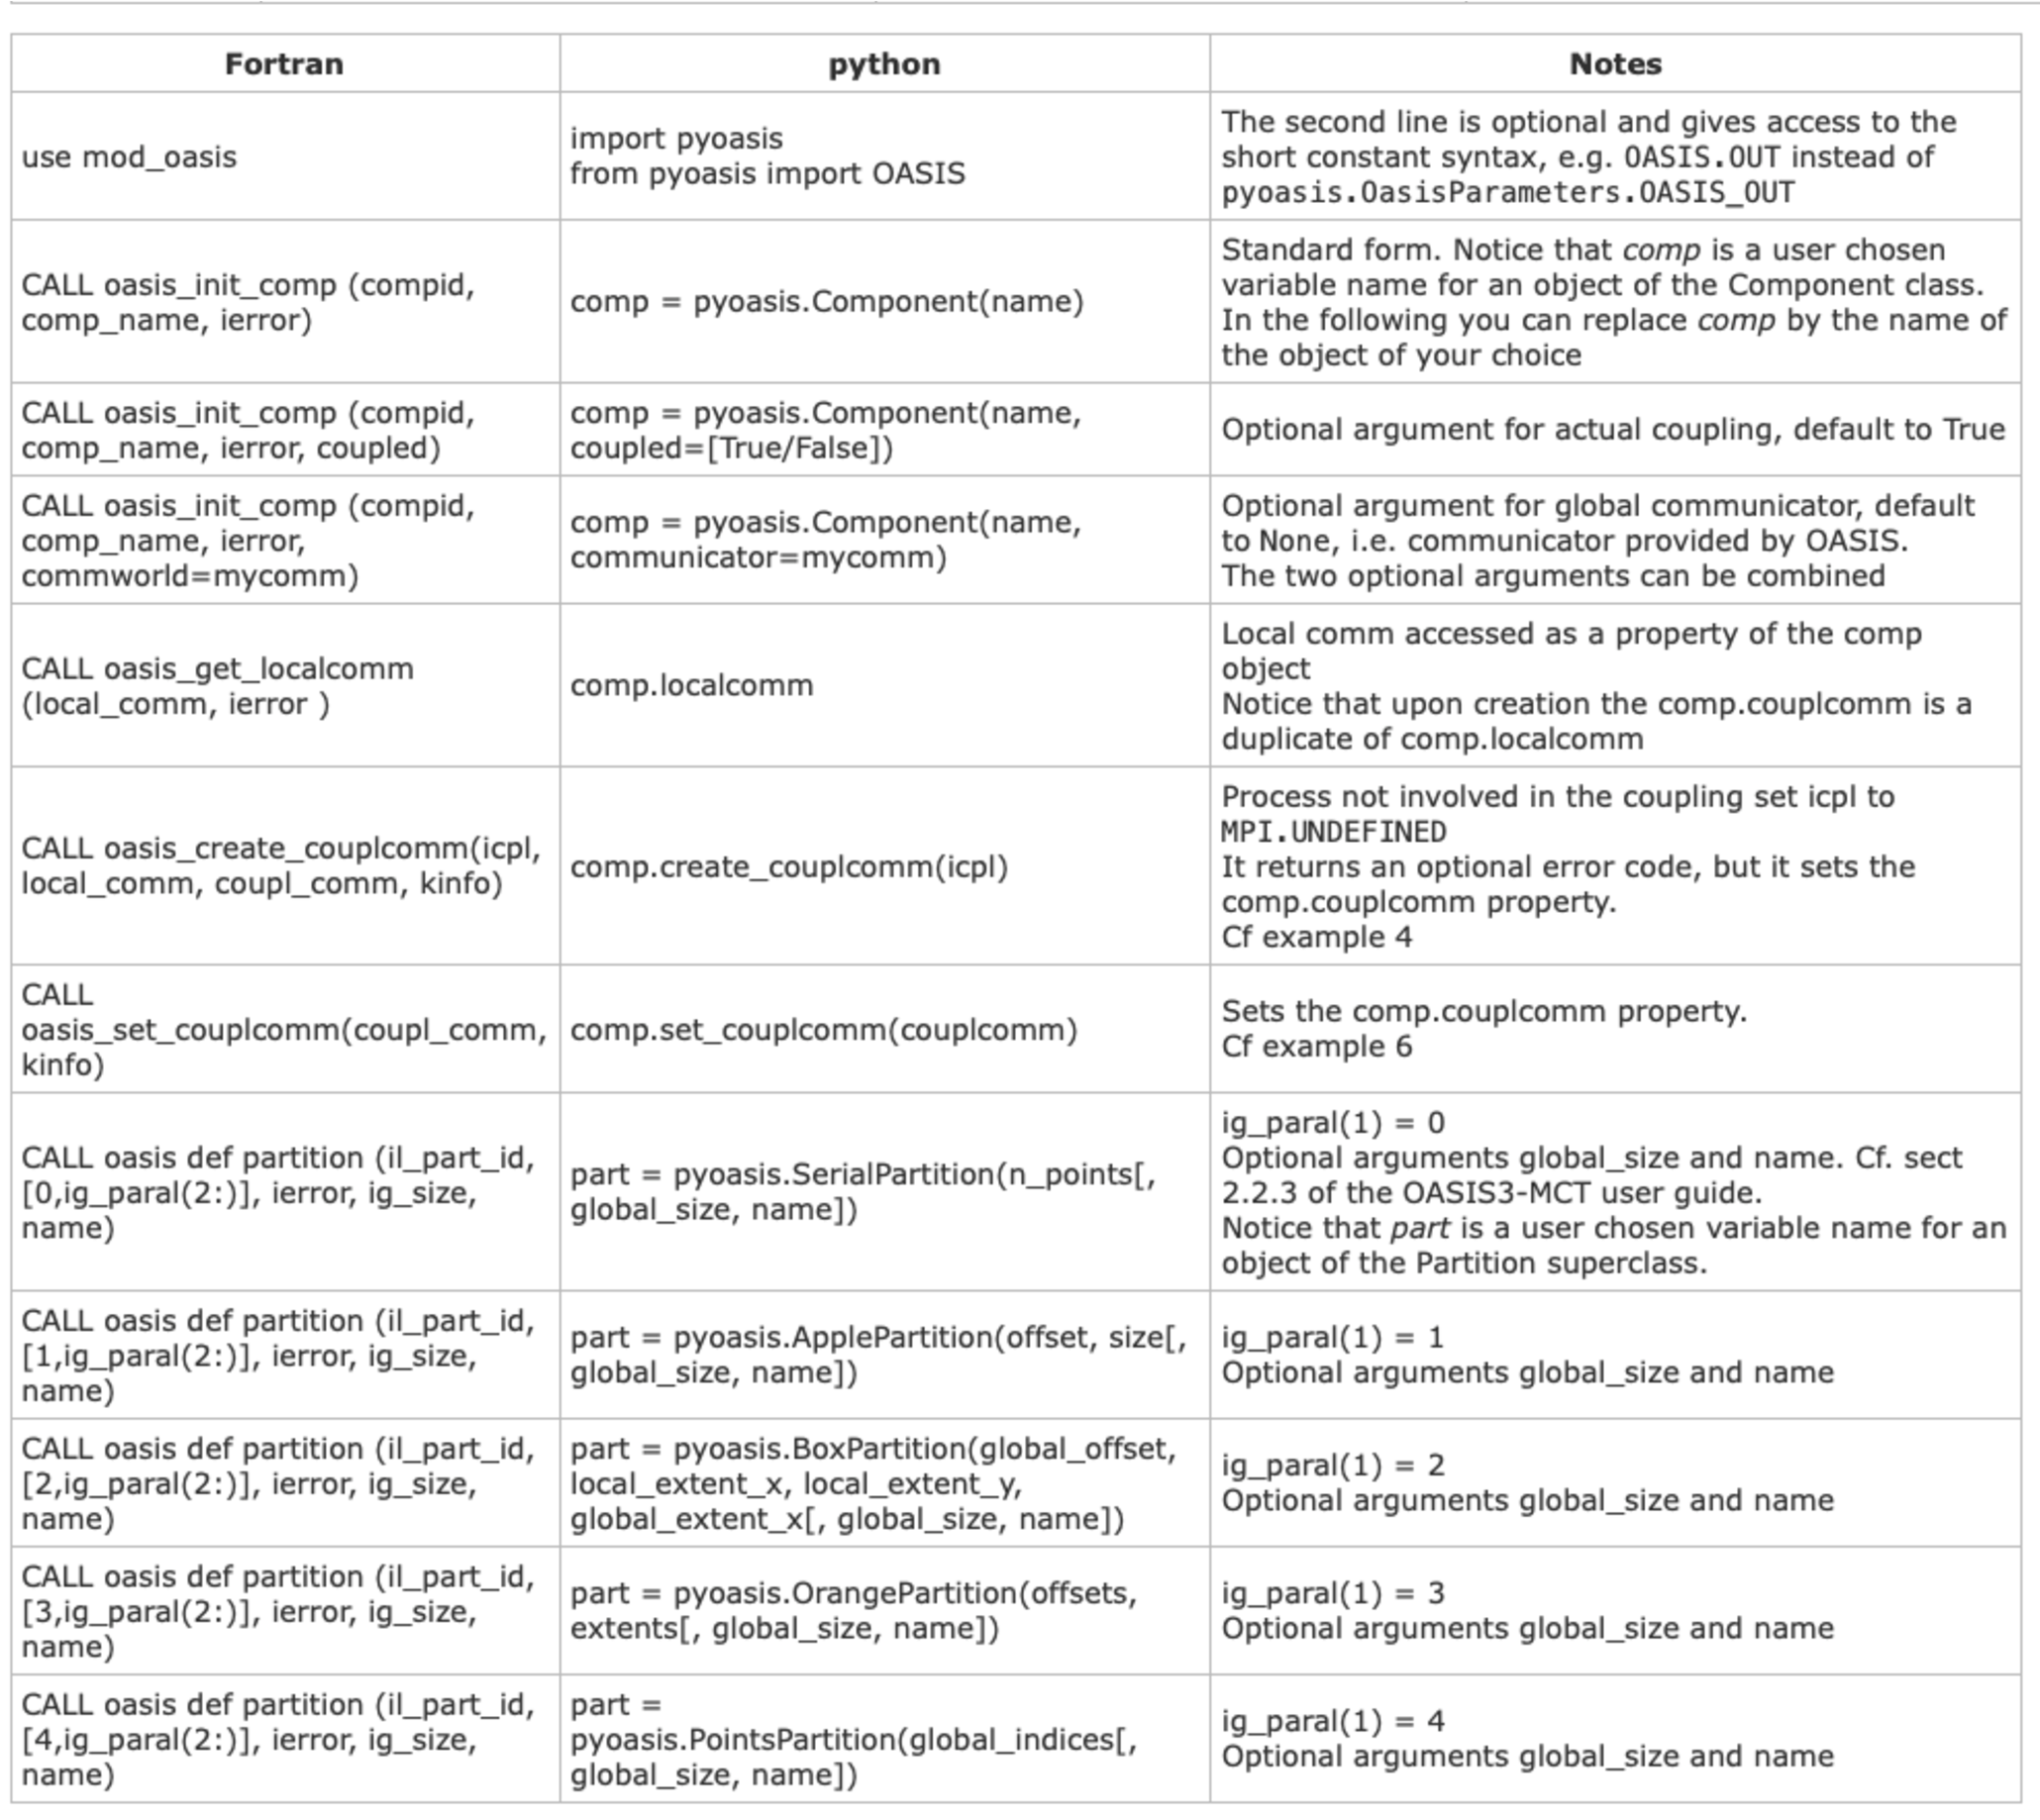
\includegraphics[scale=.45]{figures/corresp_init.pdf}
  \caption{Fortran python AP correspondence for the initialisation, communication and partition definition.}
  \label{python_corresp_init}
\end{figure}

\begin{figure}[h]
  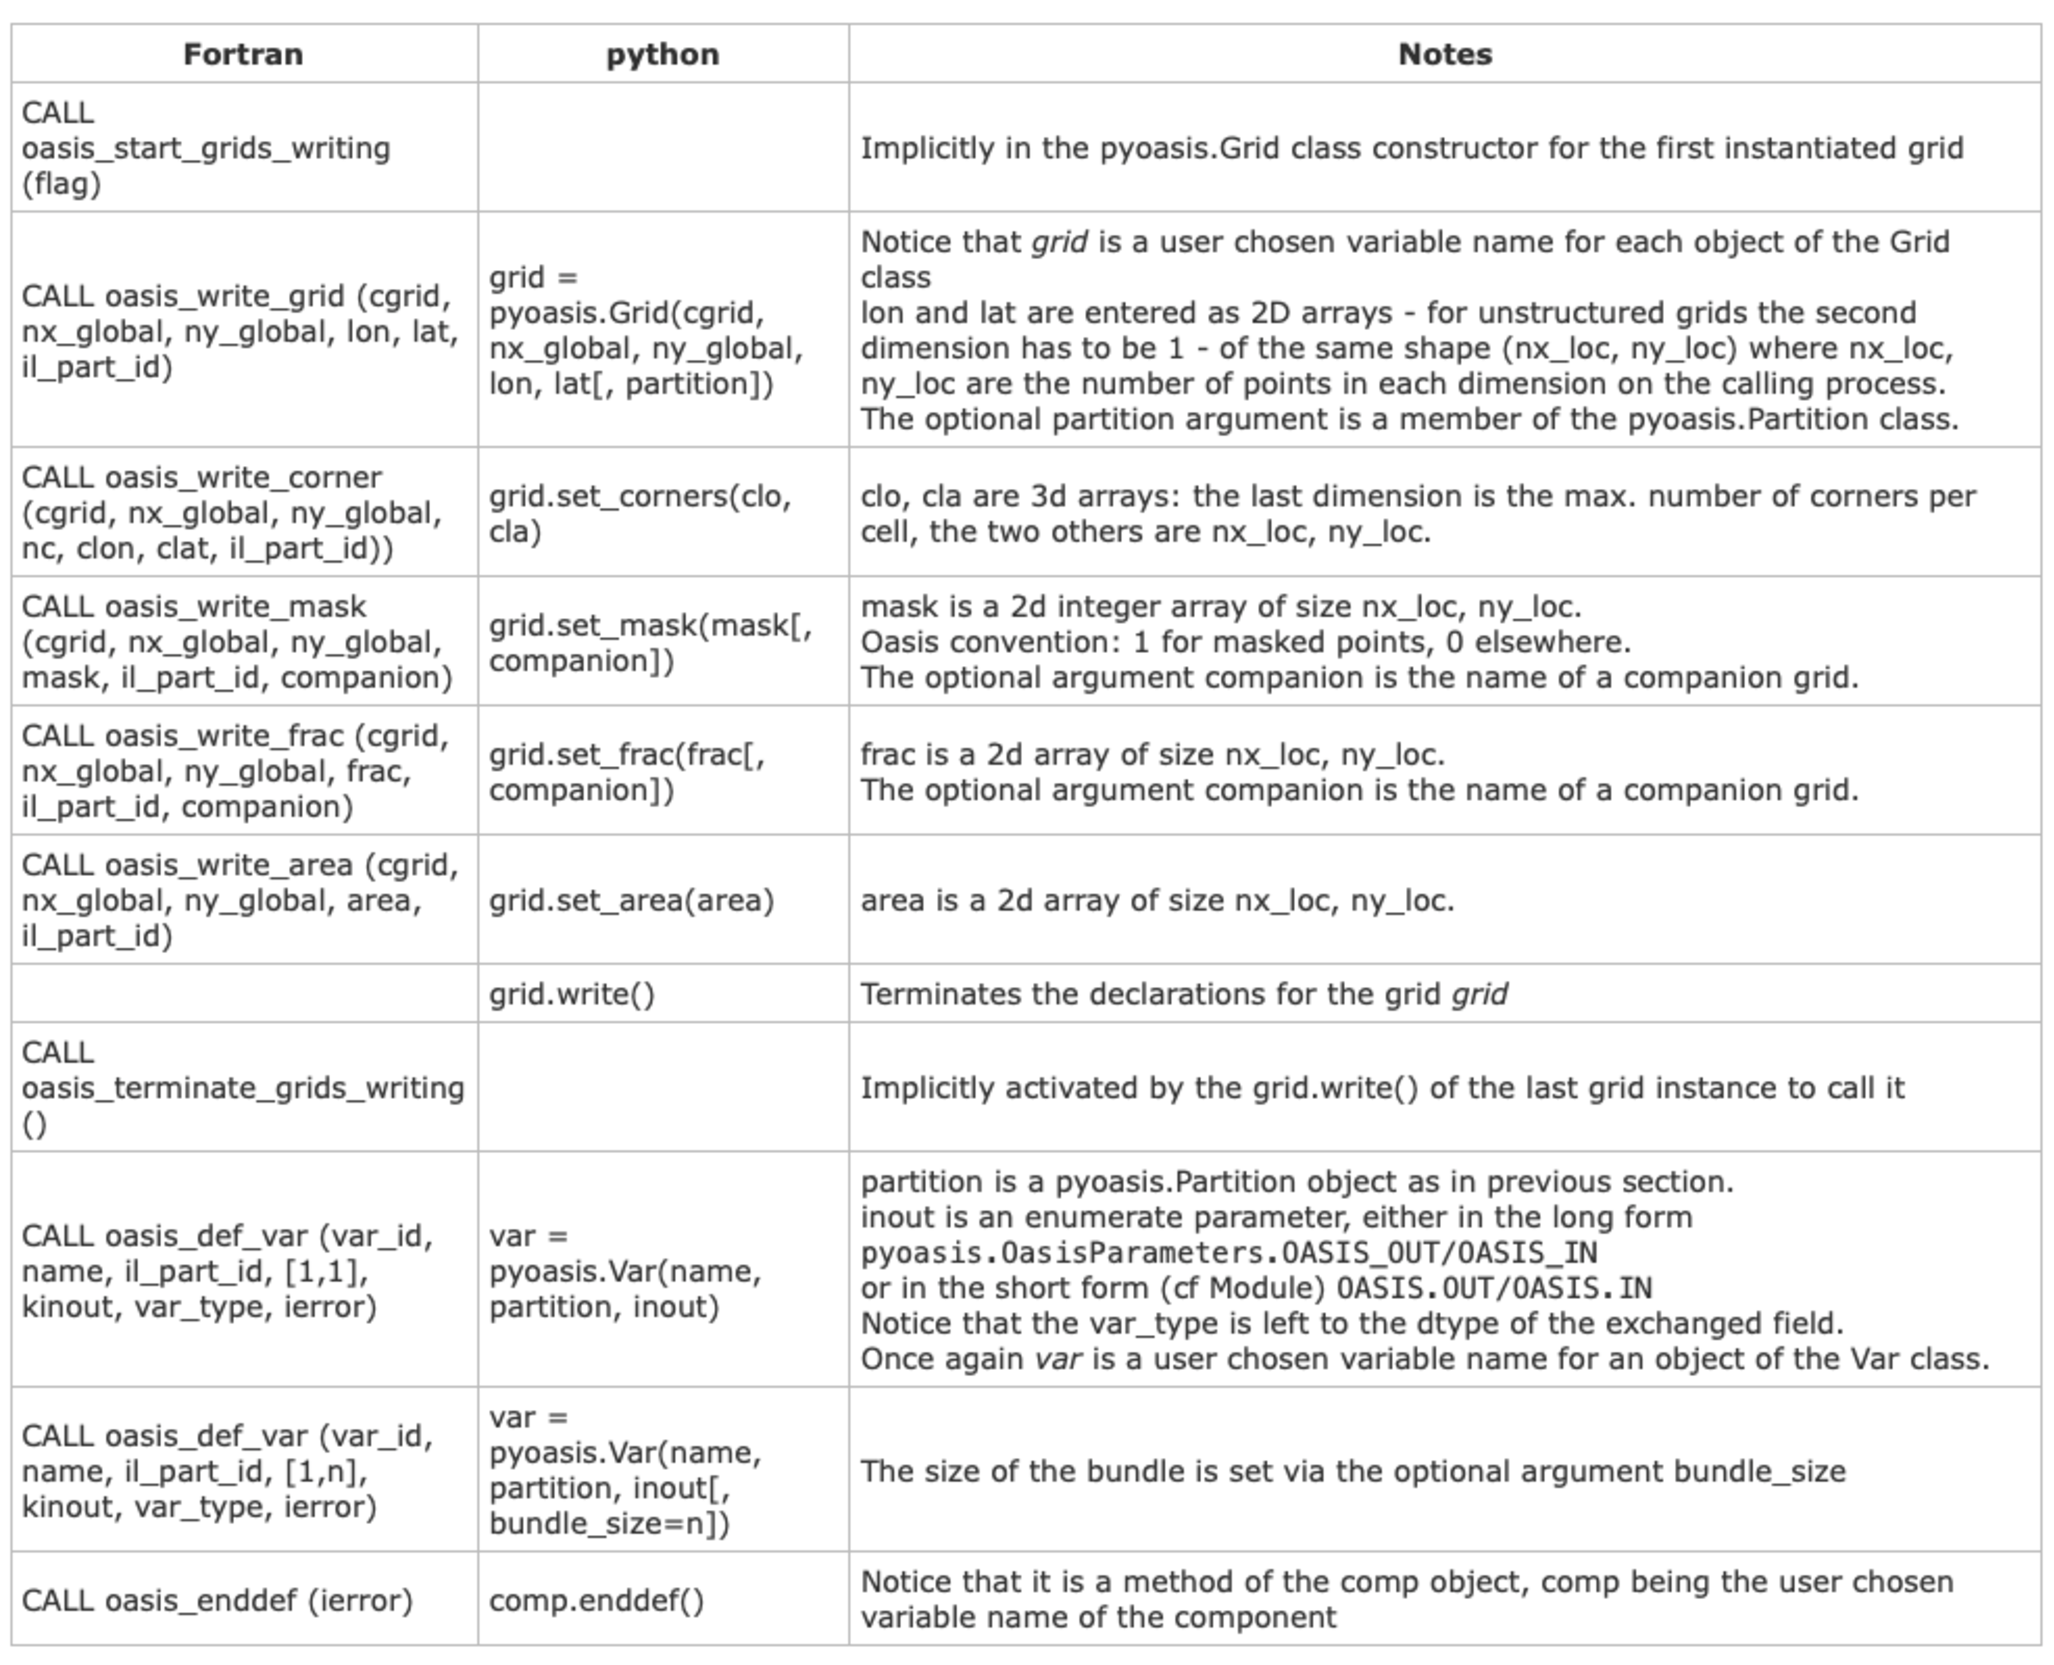
\includegraphics[scale=.45]{figures/corresp_grid.pdf}
  \caption{Fortran python AP correspondence for the grid definition, variable declaration and end of definition phase.}
  \label{python_corresp_grid}
\end{figure}

\begin{figure}[h]
  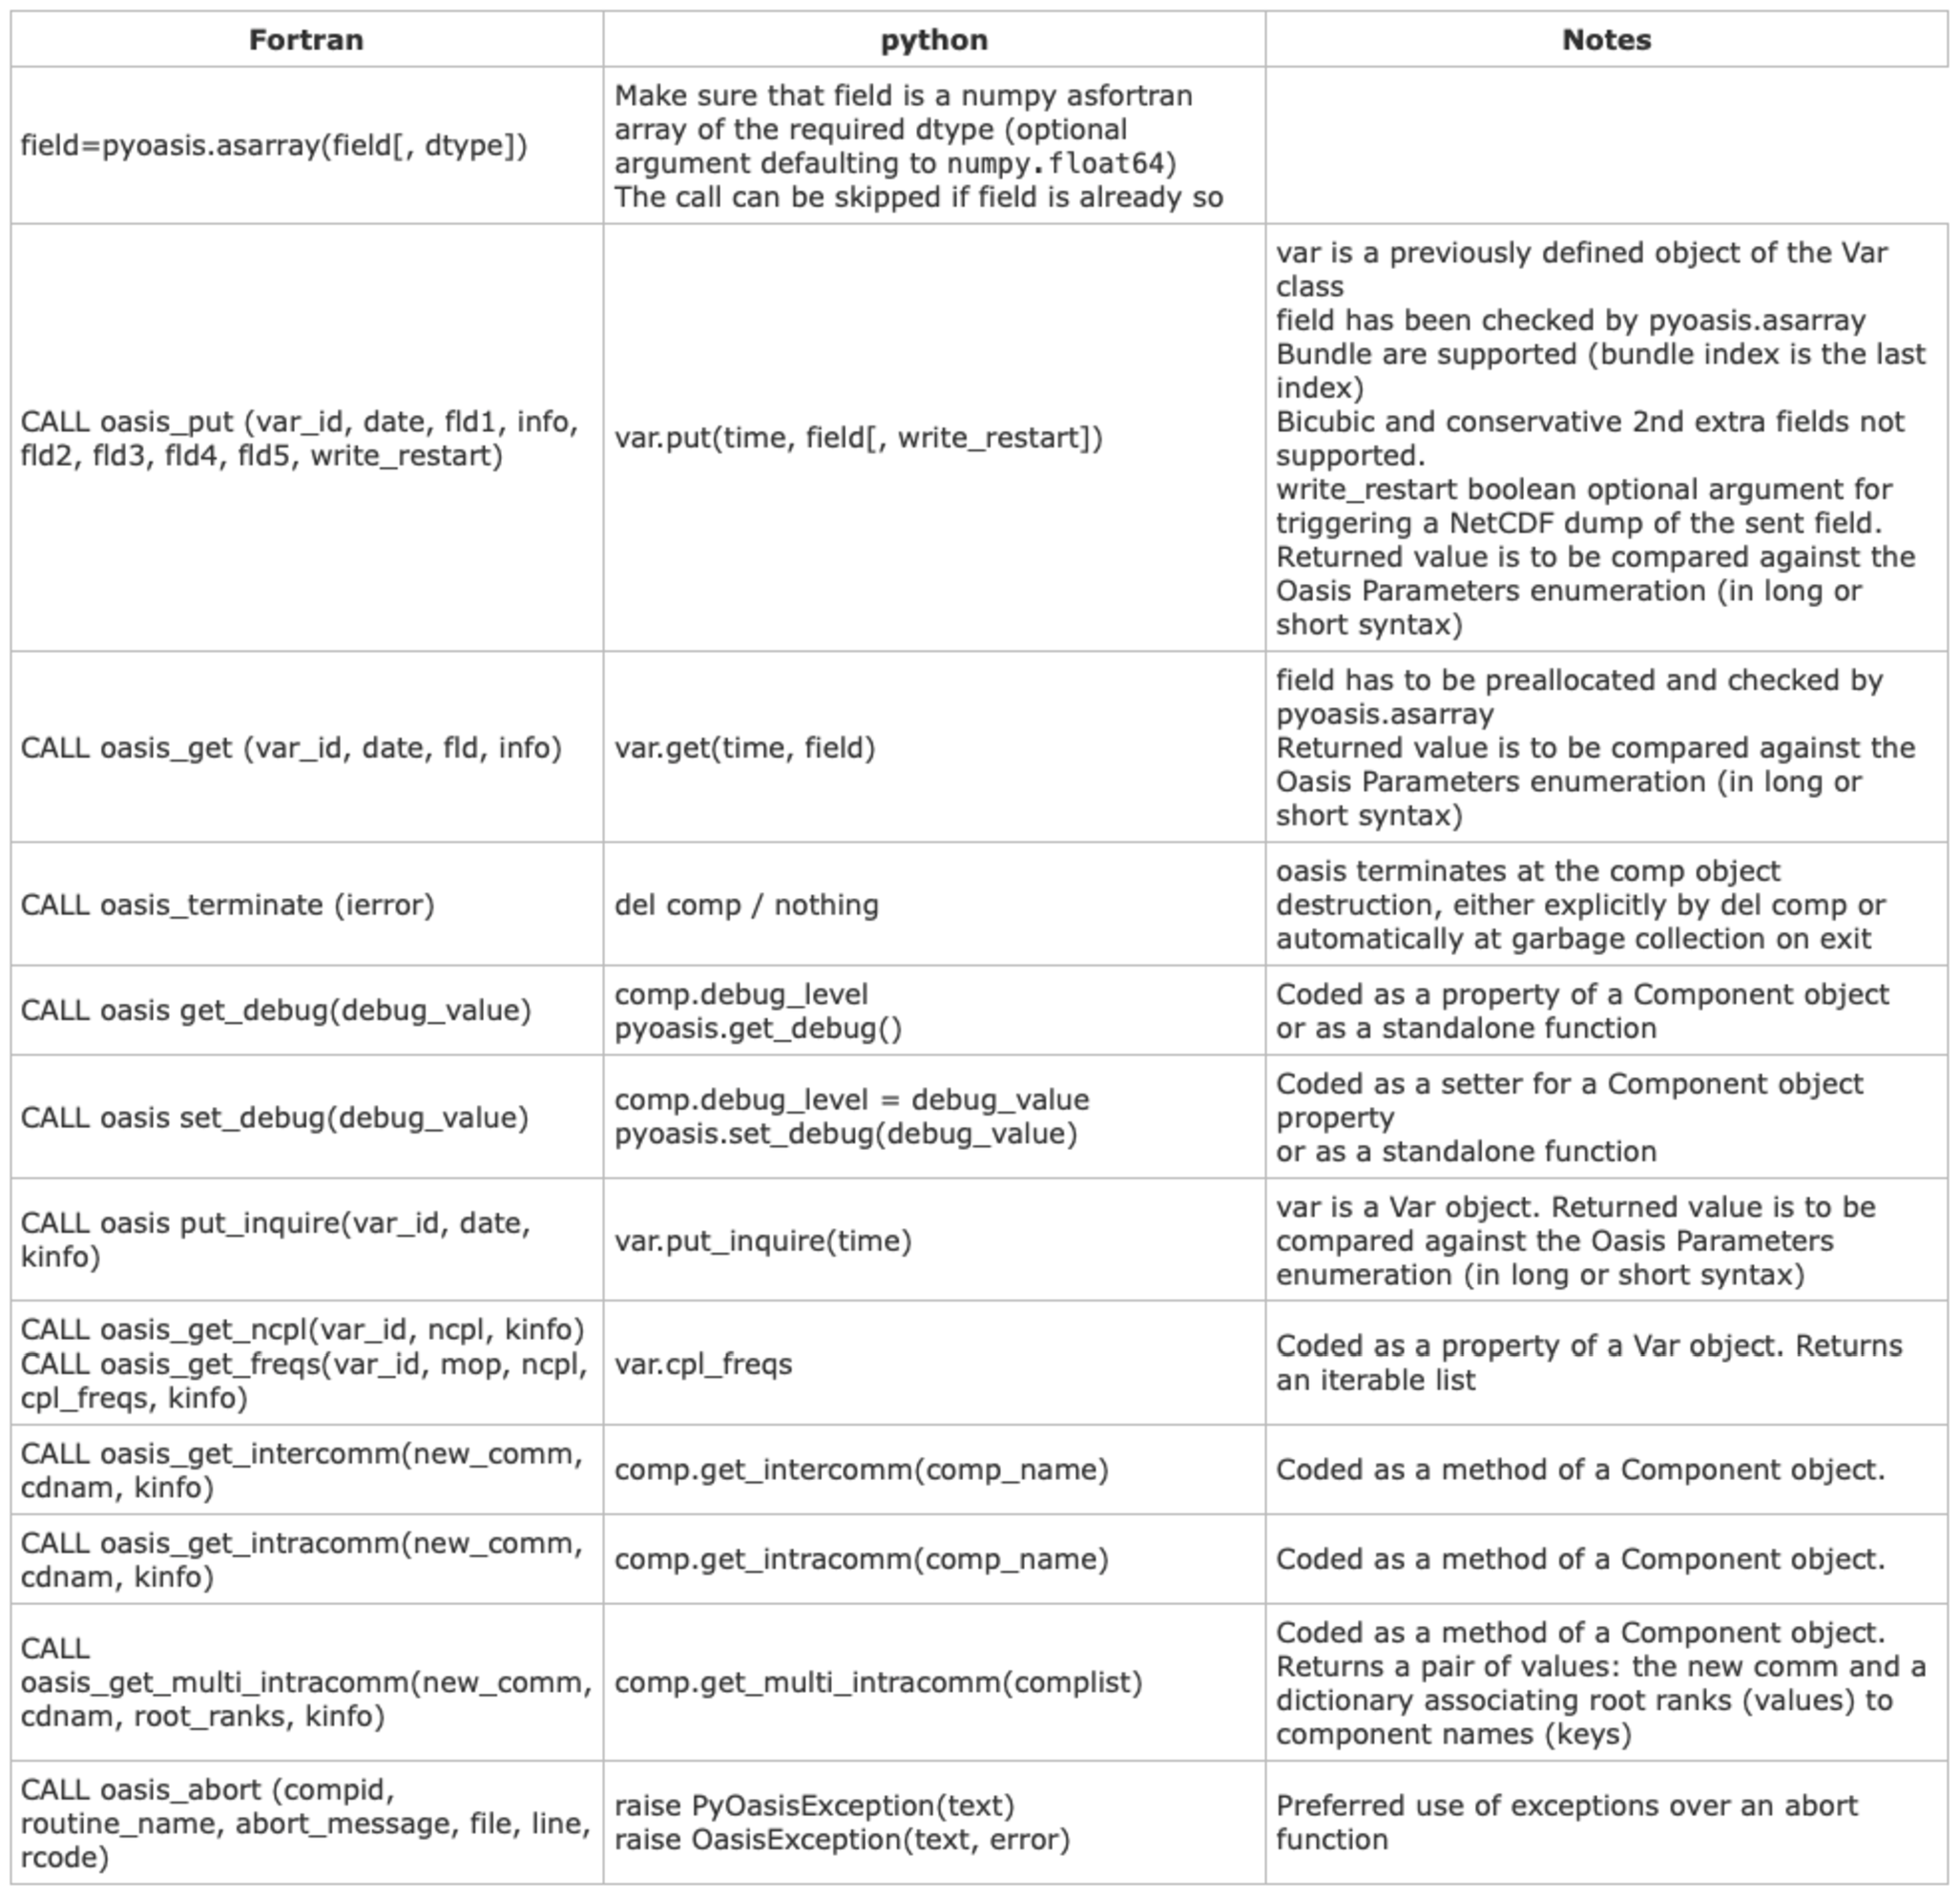
\includegraphics[scale=.45]{figures/corresp_terminate.pdf}
  \caption{Fortran python AP correspondence for the coupling field exchanges, termination and auxialiary routines.}
  \label{python_corresp_terminate}
\end{figure}

\newpage

\section{Additonal notes on coupling functionality}
\label{sec_notes}

\subsection{A brief overview of MCT}
\label{subsec_MCT}

As described elsewhere, OASIS3-MCT leverages the MCT coupling infrastructure
developed at Argonne National Laboratory.  That infrastructure is designed
to couple fields on static grids between model components.  The fields
can be decomposed using MPI across mutiple processes, and the decomposition
and number of proceses involved can be arbitrary in each component.  MCT
supports both communication of data between unique MPI non-overlapping 
communicators and
within a single MPI communicator, although these two operations are functionally
independent within MCT.  

MCT also provides the ability to map (aka interpolate or
regrid) data between grids as long as the interpolation is linear and can
be computed by a linear sparse matrix multiply.  
MCT does not compute inteporlation weights, but
it has interfaces that allow those weights to be passed into MCT.  Within
MCT, mapping and communication are also treated as independent features.

OASIS3-MCT supports both mapping and communication of data through MCT.  As
a results, mapping and coupling are implemented, in many ways, as separate
steps in the underlying implementation.  A coupling field that also requires
mapping will carry out the mapping on either the source or destination component
on the associated processes, while coupling between components will be done
either before or after mapping.  In other words, a coupling field can be 
interpolated to
the destination grid on the source processes then communicated to the destination
component OR a coupling field can be communicated to the destination component
on the source grid then mapped to the destination grid on the destination 
component.  At the present time, it is not possible to map the field as part
of the communication rearrangement, although in theory, that capability should
be possible to implement in the future, and OASIS3-MCT developers are considering
it.  The separation of mapping and communication is handled by the OASIS
layer.  Users only need to be aware of a few options that can be set to fine
tune the performance of these operations.

OASIS3-MCT also imposes a few other constraints on the usage.  MCT
does NOT support haloed communication.  There must be a 1-to-1 relationship
between grid point values on the source grid and on the destination grid.
A user cannot send a single grid point value to multiple destination gridcells
or processes via OASIS3-MCT.  The partitions defined by the user that define
the field decomposition cannot reference the same global gridcell more than once.

OASIS3-MCT does not support dynamically varying grids nor dynamically varying 
decompositions at the present time.  MCT is NOT currently setup to support those 
features.  In the future, it is possible that some dynamic grid capabilities 
might be supported through OASIS3-MCT but requirements and implementation are
still being assessed.

Since the OASIS3-MCT\_4.0 release, OASIS3-MCT includes a mixed MPI+OpenMP parallel version of the SCRIP library for the calculation of the remapping weights (see section \ref{subsec_interp}). But besides this aspect, MCT itself, and therefore the communication layer in OASIS, has only minimal OpenMP support at the
present time.  Users are discouraged from calling OASIS3-MCT {\tt oasis\_put} and {\tt oasis\_get}
from a threaded region.  And it is not possible to define a partition (decomposition)
across multiple active threads.  Most of the work that OASIS3-MCT does related to decomposition rearrangement for communication or mapping per se is MPI-based.  There
are some floating point operations in the sparse matrix multiple as well as in
some of the OASIS transforms; but generally, these are highly parallel and
would often not benefit from use of OpenMP.  OASIS3-MCT is designed primarily to
support large memory parallel applications that require efficient and scalable
coupling and mapping capabilities.

MCT only supports coupling of integer or floating point data.  Fields based on
logicals and character strings cannot be coupled.

\subsection{Coupling scalar values}
\label{subsec_scalar}

OASIS3-MCT does not have a distinct feature to support scalar coupling.  By
scalar coupling, we mean  scalar variables such as date and time,
logical flags, integer or real parameters, or other scalar data that might be
defined identically across all MPI tasks in a component or even just on the
root task or a subset of tasks.  
It is often desirable to communicate scalar data between components
to coordinate scientific or technical features.  There isn't a feature that
supports this type of coupling specifically, but it is possible to do so using  
available interfaces.  The most robust implementation is probably to setup
root to root coupling of scalars between components.  To do so :

\begin{itemize}
\item Determine the number and type of scalars to couple
\item Allocate an array in each component of that size
\item Initialize a partition using the POINTS approach (see section \ref{subsubsec_pointspart}) with the size of the array assigned to the root process in each component and no portion of the partition allocated to other processes.  
\item Define coupling field names for use in both the model components and the namcouple file and declare variables as usual.  Create a set of namcouple inputs.  You will not need any mapping.
\item Use the {\tt oasis\_get} and {\tt oasis\_put} interfaces to communicate data between components.
\item If required, broadcast the scalars after being received from the root process to the other processes, outside the OASIS3-MCT layer.
\end{itemize}

This can be extended as needed to send or receive from non root processes.  But
you cannot send the scalar data to multiple processes as this violates the halo
restriction in MCT.  Users need to be aware which processes contain valid scalar
data both on the source and destination side and to manage data synchronization 
between processes within a component outside the OASIS3-MCT layer.

\vspace{-0.3cm}
\subsection{The lag concept}
\label{subsec_lag}

Using the OASIS3-MCT coupling library, the user has the flexibility
to reproduce different coupling algorithms defining {\tt LAG} values for the different coupling fields . 
In the components, the
sending and receiving routines, respectively {\tt oasis\_put} and {\tt
  oasis\_get}, can be called at each component timestep, with the
appropriate {\tt date} argument giving the actual time (at the
beginning of the timestep), expressed in number of seconds since the
start of the run, or in any other time units as long as the same are
used in all components and in the {\it namcouple} (see section
\ref{prismput}). This {\tt date} argument is automatically analysed by
the coupling library and depending on the coupling period and the lag chosen by the user for the coupling field in the {\it namcouple} ({\tt LAG}), different coupling algorithms can be reproduced
without modifying the component codes themselves.

The lag ({\tt LAG}) must be
expressed in the time unit used (that must be the same in the components
and in the {\it namcouple}, see section \ref{prismput}) and can be
positive or negative but should never be larger (in absolute
magnitude) than the coupling period of any field due to problems with
restartability and dead-locking. When a component calls a {\tt
  oasis\_put}, the value of the lag is automatically added to the
value of the {\tt date} argument and the ``put'' is actually performed
when the sum {\tt date+lag} is a coupling time; in the target
component, this ``put'' will match a {\tt oasis\_get} for which the
{\tt date} argument is the same coupling time.
% A positive lag indicates the put will occur sooner than zero lag and
% a negative lag tells the coupler to send the data later than zero
% lag.
So the lag only shifts the time at which the data is sent but not
the time at which the data is received.
 
When the lag is positive, a restart file must be available to initiate
the coupling.  For a field with positive lag, the source
component automatically reads the field in the restart file
during the coupling initialization phase (below the {\tt
  oasis\_enddef}) and send the data to match the {\tt oasis\_get}
performed at time=0 in the target component. The final coupling
data on the source side will then be automatically written to the
restart file for use in the next run\footnote{When there is a lag, the first and last instance of the source field
in the debug netCDF file (EXPOUT fields, see section
\ref{subsec_namcouplesecond}) always correspond respectively to the
field read from and written to the restart file.}.

On the 4 figures in this section, short black arrows correspond to
  {\tt oasis\_put} or {\tt oasis\_get} called in the component
  that do not lead to any ``put" or receiving action; long black
  arrows correspond to {\tt oasis\_put} or {\tt oasis\_get} called in
  the components that do actually lead to a ``put" or ``get''
  action; long red arrows correspond to {\tt oasis\_put} or {\tt
    oasis\_get} called in the component models that lead to a reading
  or writing of the coupling field from or to a coupling restart file.
 
\begin{enumerate}

\item LAG concept first example
 
  A first coupling algorithm, exploiting the LAG concept, is
  illustrated on figure \ref{fig:lag_concept_1}.

  \begin{figure}
    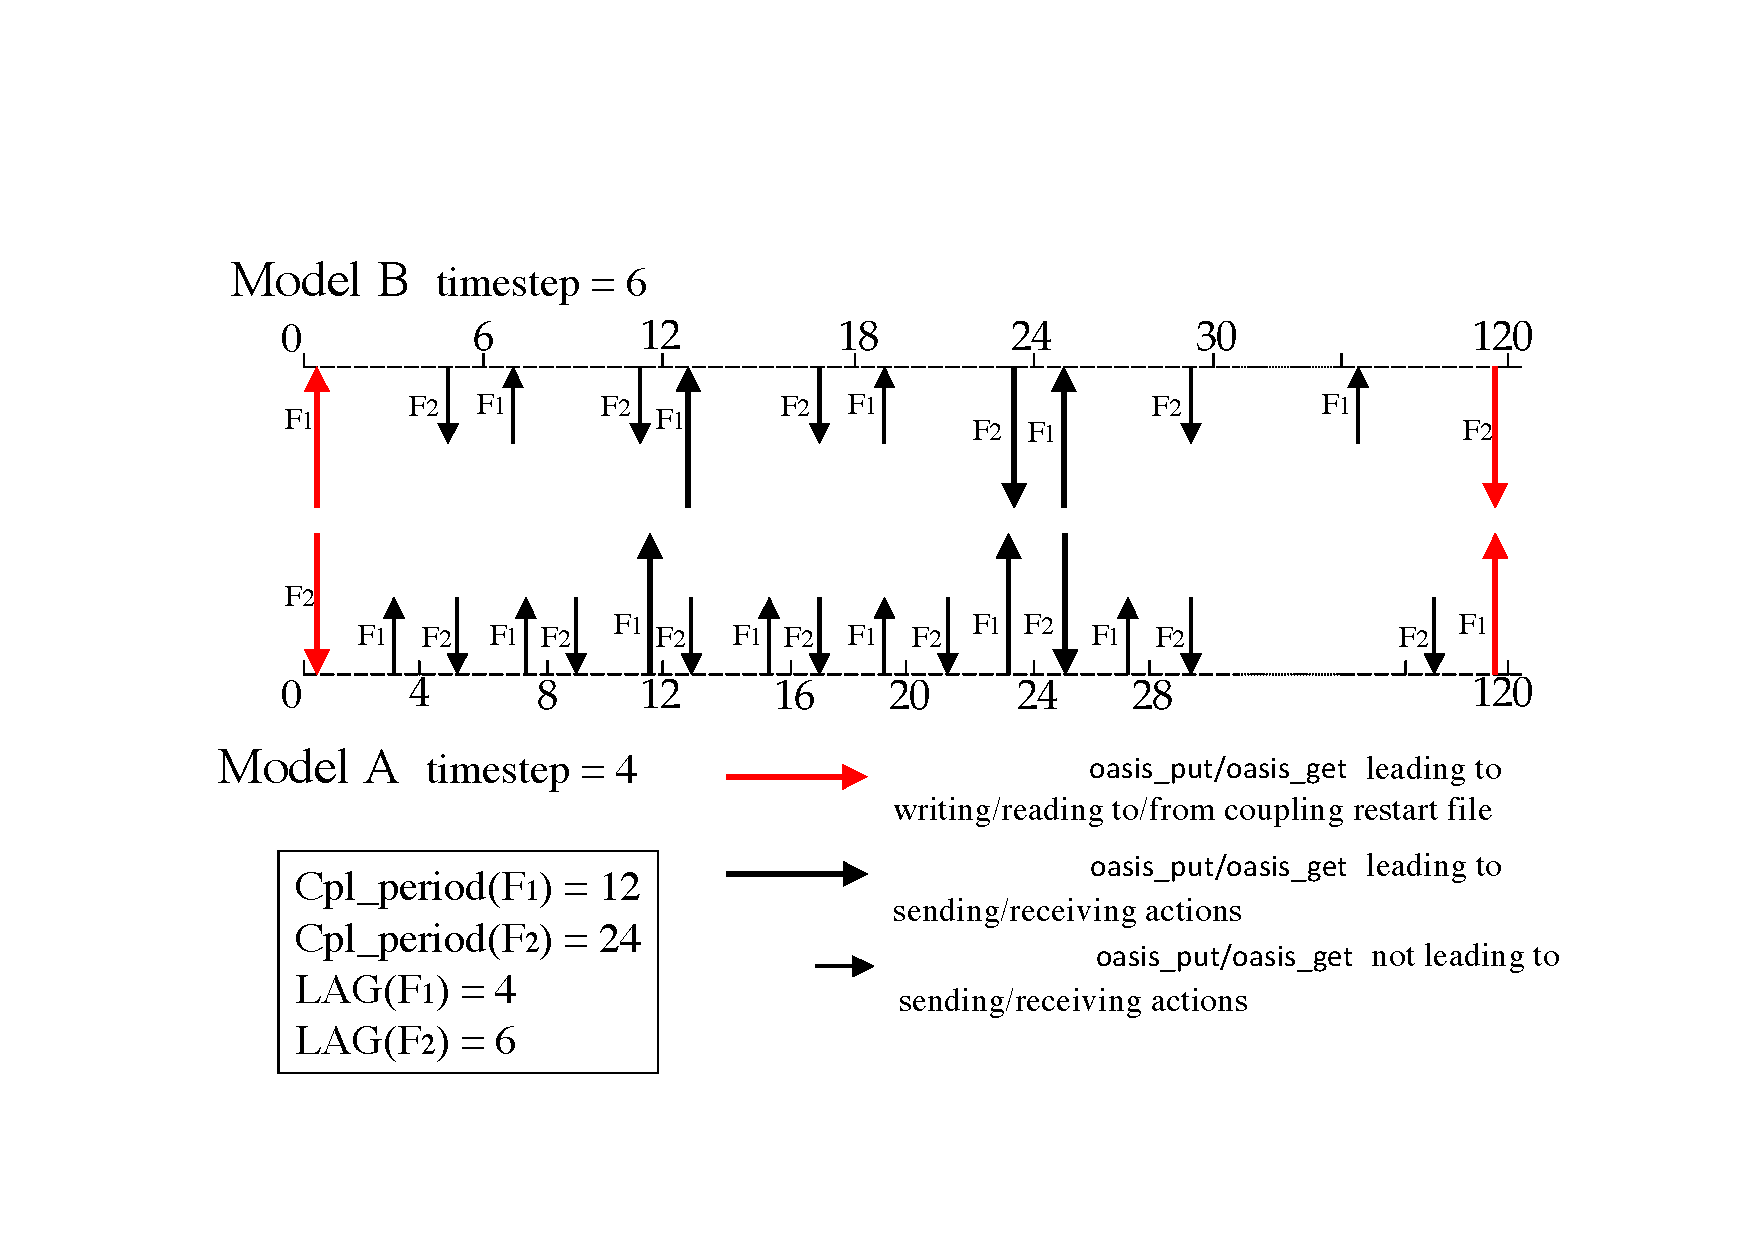
\includegraphics[scale=.6]{figures/fig_lag_concept_1}
    \caption{LAG concept first example}
    \label{fig:lag_concept_1}
  \end{figure}

  During a coupling timestep, model A receives $F_2$ and then sends
  $F_1$; its timestep length is 4. During a coupling timestep, model B
  receives $F_1$ and then sends $F_2$; its timestep length is 6.
  $F_1$ and $F_2$ coupling periods are respectively 12 and 24. If
  $F_1$/$F_2$ ``put" action by model A/B was used at a coupling
  timestep to match the model B/A ``get" action, a deadlock would
  occur as both models would be initially waiting on a ``get"
  action. To prevent this, $F_1$ and $F_2$ produced at the timestep
  before have to be used to match respectively the model B and model A
  ``get" actions.

  This implies that a lag of respectively 4 and 6 seconds must be
  defined for $F_1$ and $F_2$. For $F_1$, the {\tt oasis\_put}
  performed at time 8 and 20 by model A will then lead to ``put"
  actions (as 8 + 4 = 12 and 20 + 4 = 24 which are coupling periods)
  that match the ``get" actions performed by {\tt oasis\_get} called by model B
  at times 12 and 24.  For $F_2$, the {\tt oasis\_put}
  performed at time 18 by model B then leads to a ``put" action (as 18
  + 6 = 24 which is a coupling period) that matches the ``get" action
  performed at time 24 by the {\tt oasis\_get} called by model A.

  At the beginning of the run, as their LAG index is greater than 0,
  the first {\tt oasis\_get} of $F_1$ and $F_2$ will automatically be
  fulfilled with fields read from their respective coupling restart
  files. The user therefore has to create those coupling restart files
  before the first run in the experiment. At the end of the run, $F_1$
  having a lag greater than 0, is automatically written to its
  coupling restart file below the last $F_1$ {\tt oasis\_put} as the
  {\tt date+lag} equals the total run time. The analogue is true for
  $F_2$. These coupling restart fields will automatically be read in at the beginning
  of the next run below the respective {\tt oasis\_get}.

\item LAG concept second example

  A second coupling algorithm exploiting the LAG concept is
  illustrated on figure \ref{fig:lag_concept_2}. During its timestep,
  model A receives $F_2$, sends $F_3$ and then $F_1$; its timestep
  length is 6. During its timestep, model B receives $F_1$, receives
  $F_3$ and then sends $F_2$; its timestep length is also 6.  $F_1$,
  $F_2$ and $F_3$ coupling periods are both supposed to be equal to
  12.
 
  \begin{figure}
    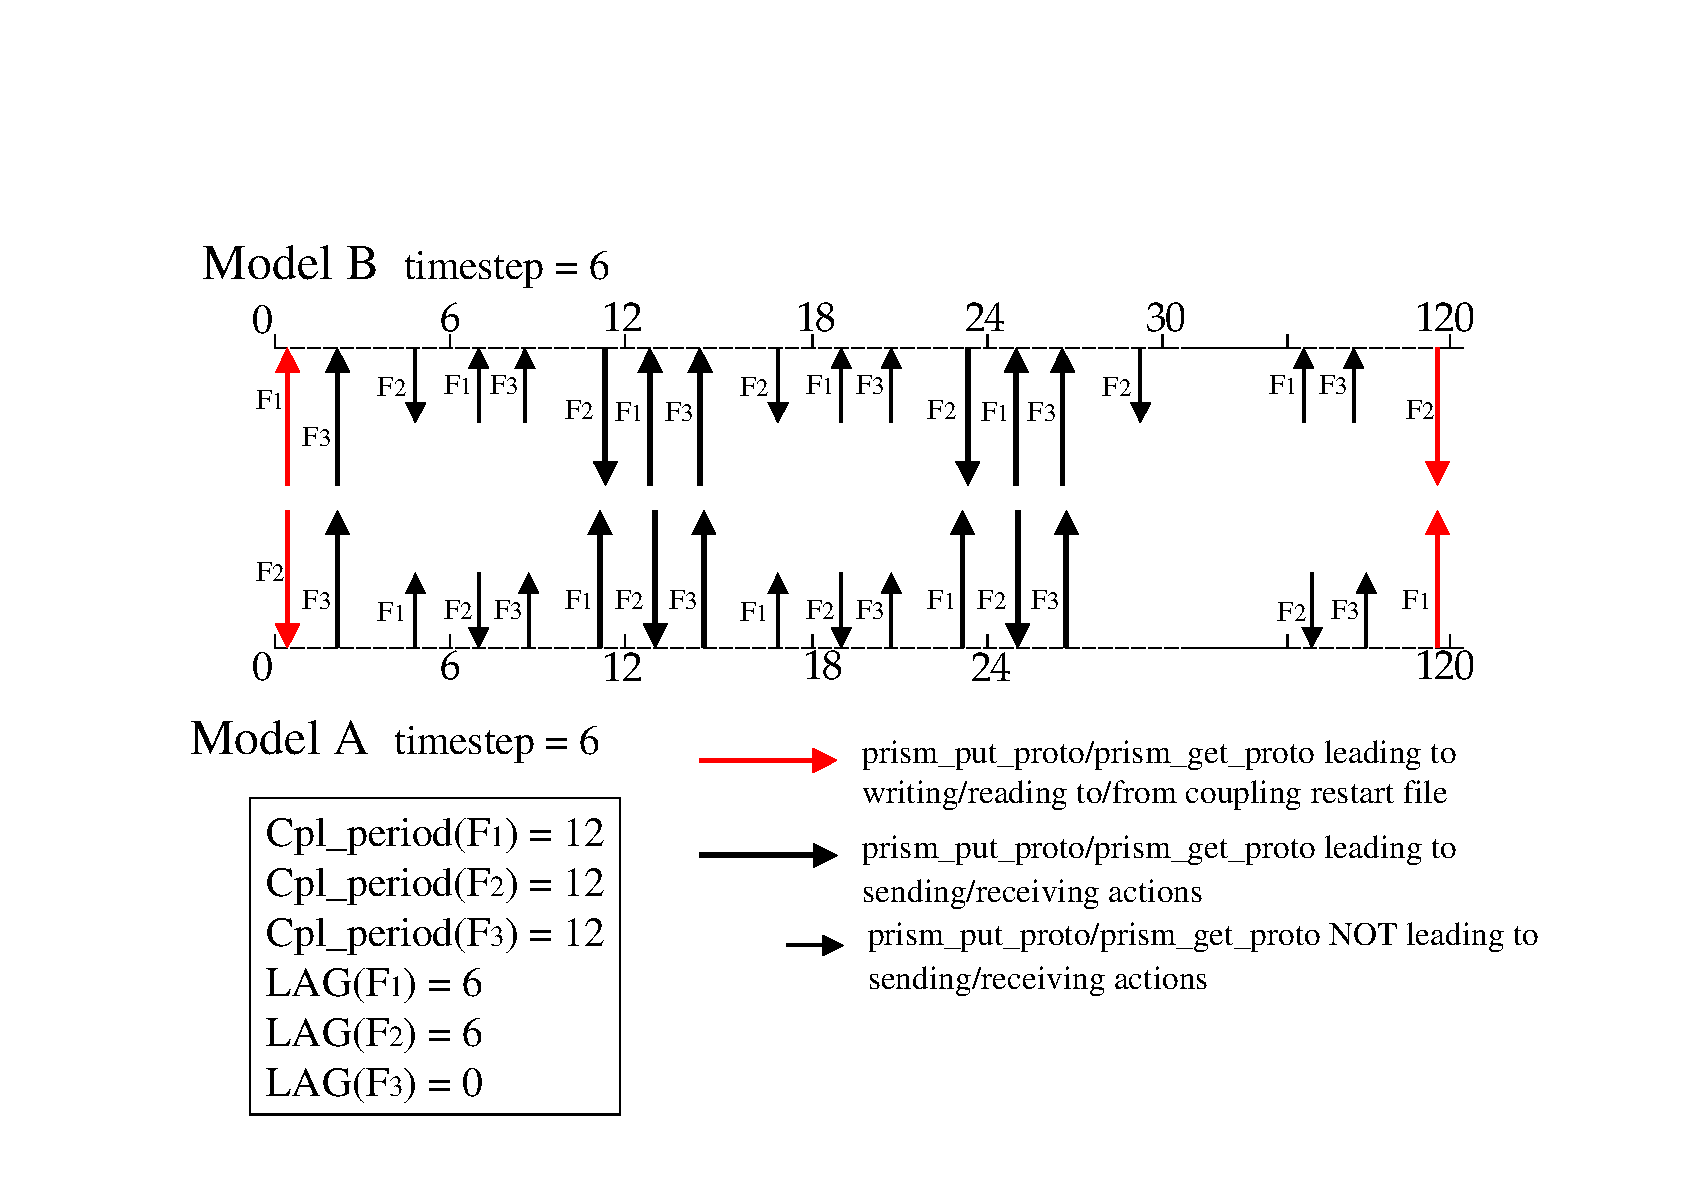
\includegraphics[scale=.6]{figures/fig_lag_concept_2}
    \caption{LAG concept second example}
    \label{fig:lag_concept_2}
  \end{figure}

  For $F_1$ and $F_2$ the situation is similar to the first
  example. Without any lag specified and without any restart file, a deadlock
  would occur as both models would be waiting on a ``get" action. To
  prevent this, $F_1$ and $F_2$ produced at the timestep before have
  to be used to match the model A and model B ``get" actions, which
  means that a lag of 6 must be defined for both $F_1$ and $F_2$. For
  both coupling fields, the {\tt oasis\_put} performed at times 6 and
  18 by the source model then lead to ``put" actions (as 6 + 6 = 12
  and 18 + 6 = 24 which are coupling periods) that match the ``get"
  action performed at time 12 and 24 by the {\tt oasis\_get} called
  by the target model.

  For $F_3$, sent by model A and received by model B, no lag needs to
  be defined: the coupling field produced by model A at the coupling
  timestep can be ``consumed'' by model B without causing a deadlock
  situation.

  As in the first example, the {\tt oasis\_get} performed at the
  beginning of the run for $F_1$ and $F_2$, will automatically receive
  data read from their coupling restart files, and the last {\tt
    oasis\_put} performed at the end of the run automatically write
  them to their coupling restart file. For $F_3$, no coupling restart
  file is needed.

  We see here how the introduction of appropriate LAG indices results
  in receiving in the target component the coupling fields produced by the
  source component the time step before; this is, in some coupling
  configurations, essential to avoid deadlock situations.

\end{enumerate}

\vspace{-0.3cm}
\subsection{The sequence concept}
\label{subsec_sec}

The order of coupling operations in the system is determined solely by
the order of calls to send ({\tt oasis\_put} or ``put'') and receive ({\tt oasis\_get} or ``get'') data in the components
in conjunction with the setting of the lag in the {\it namcouple}.
Data that is received is always blocking while data that is sent is non-blocking with respect to the component making that call.  It
is possible to deadlock the system if the relative orders of puts and
gets in different components are not compatible.

With OASIS3-MCT, the sequence (SEQ) index in the {\it namcouple} file
now provides the coupling layer with an ability to detect a deadlock
before it happens and exit.  It does this by tracking the order of get
and put calls in components compared to the SEQ specified in the {\it
  namcouple}.  If there are any inconsistencies, the component will abort
gracefully with a useable error message before the system deadlocks.
If there are any coupling dependencies in the system, use of the SEQ
index is recommended for diagnosis but has no impact on the ultimate
solution and is NOT required.

In the following two examples, there are two
models, each ``put" a field to the other at every coupling period
without any lags.  In the first case, there is no dependency as each
model first sends and then receives some data.

\begin{verbatim}
     model1        model2
     ------        ------
    put(fld1)     put(fld2)
    get(fld2)     get(fld1)
\end{verbatim}

In this
case, there is no sequencing dependency and the value of SEQ must be
identical (or unset) in the {\it namcouple} description of the fld1
and fld2 coupling.  If by mistake, SEQ is set to 1 for fld1 and 2 for fld2, 
then the coupled model will abort because at runtime, the coupler will
detect in model 2 that fld2 was sent before fld1 was received which
is out of sequence as defined by the SEQ settings.

In the next example, there is a dependency in the sequencing.

\begin{verbatim}
     model1        model2
     ------        ------
    put(fld1)     get(fld1)
                  fld2=g(fld1)
    get(fld2)     put(fld2)
\end{verbatim}

In model2, fld2 depends on fld1. If SEQ is not used and if, for example, model1 does not have the
consistent ordering of the put and get shown above (required by model2), then the models would deadlock and hang. If this dependency is known, there is a benefit in setting SEQ=1 for fld1 and SEQ=2 for fld2; at
runtime, if the sequencing of model1 or model2 does not match the
above diagram, then the  coupling layer will detect it and will exit gracefully with an error message.

Again, the SEQ namecouple setting is only diagnostic and is not
required.






\include{UG3_Namcouple_generation}
\include{UG4_Transformations}
\newpage
\chapter{OASIS3-MCT auxiliary data files}
\label{sec_auxiliary}

OASIS3-MCT uses auxiliary data files, defining the
grids of the models being coupled, or containing coupling field 
restart values or input data values or remapping weights and
addresses. These files can be created by the user before the run or by OASIS3-MCT itself in the initialisation phase.

\section{Grid data files}
\label{subsec_griddata}

OASIS3-MCT requires grid data files {\em grids.nc, masks.nc} and {\em
  areas.nc} for certain operations:
\begin{itemize}
  \item{\em grids.nc} and {\em masks.nc} for all {\tt SCRIPR} and {\tt YAC} regriddings (see
    section \ref{subsec_interp}) ;
  \item {\em areas.nc} for {\tt SCRIPR} conservative remapping
when the normalisation by the true area of the cells is 
activated (i.e. {\tt DESTARTR}, {\tt DESTNNTR}, {\tt FRACARTR}, or
{\tt FRACNNTR}) ; for {\tt YAC} source to target mapping method {\tt SPMAP} when the option to use areas defined in {\em areas.nc} is activated ({\tt src\_radius} or {\tt tgt\_radius} = {\tt FILE}), see section \ref{subsec_interp};
\item {\em masks.nc} and {\em areas.nc} for global {\tt
    CONSERV} operation, see section \ref{subsec_cooking}.
\end{itemize}

These NetCDF files can
be created by the user before the run or can be written directly at
run time by the component model processes in the initialisation phase
using the grid
data definition routines (see section \ref{subsubsec_griddef}).

The arrays containing the grid information are dimensioned {\tt (nx,
  ny)}, where {\tt nx} and {\tt ny} are the grid first and second
dimension.  Unstructured grids or other grids expressed with 1D
vectors are supported by setting {\tt nx} to the total number of grid
points and {\tt ny} to 1.

\begin{enumerate}

\item {\em grids.nc}: contains the model grid longitudes and latitudes
  in double precision {\tt REAL} arrays. The array names must be 
  composed of a prefix (4 characters), given by the user in the {\it
    namcouple} on the second line of each field (see section
  \ref{subsec_namcouplesecond}), and of a suffix,{\tt .lon} or {\tt .lat}, for respectively the grid point
  longitudes or latitudes.

  If the {\tt YAC/CONSERV} or {\tt SCRIPR/CONSERV} remapping is specified, longitudes and
  latitudes for the source and target grid {\bf corners} must also be
  available in the {\em grids.nc} file as double precision {\tt
    REAL} arrays dimensioned {\tt (nx,ny,nc)}
  where {\tt nc} is is the maximum number of corners 
  (in the counterclockwize sense, starting by any corner) over all cells; 
   {\tt nc} can be any number. For cells that do not have the maximum 
  number of distinct corners, we recommend to repeat the last corner 
  as many times as needed to describe  {\tt nc} corners.
  The names of the arrays must be composed of the grid prefix
  and the suffix {\tt .clo} or {\tt .cla} for respectively the grid corner
  longitudes or latitudes.  

  % For source grids of Logically Rectangular LR type only, the grid
  % corners will however be automatically calculated and stored by
  % OASIS if they are not initially available in {\em
  %   grids.nc}\footnote{Tip: to automatically calculate the corners
  %   of a Logically Rectangular LR target grid, use the corresponding
  %   reverse remapping in which the current target grid becomes the
  %   source grid.}.
 
  Longitudes must be given in degrees East in the interval -360.0 to
  720.0. Latitudes must be given in degrees North in the interval
  -90.0 to 90.0. Note that if some grid points overlap, it is
  recommended to define those points with the same number (e.g. 360.0
  for both, not 450.0 for one and 90.0 for the other) to ensure
  automatic detection of overlap by OASIS3-MCT.
 
  The corners of a cell cannot be defined modulo 360 degrees. For
  example, a cell located over Greenwich will have to be defined with
  corners at -1.0 deg and 1.0 deg but not with corners at 359.0 deg
  and 1.0 deg.
 
  Cells larger than 180.0 degrees in longitude are not supported.
  
  Longitudes and latitudes of grid points or corners can be defined through the {\tt oasis\_write\_grid} or {\tt oasis\_write\_corner} API routines respectively,  see section \ref{subsubsec_griddef}.
 
\item {\em masks.nc}: contains the masks for all component model grids
  in {\tt INTEGER} arrays.
{\bf Be careful to follow the historical
    OASIS3-MCT convention: 0 = not masked (i.e. active), 1 = masked
    (i.e. not active) for each grid point}. The array names must be
  composed of the grid prefix and the suffix ``.msk''. Mask can be defined through the {\tt oasis\_write\_mask} API routine, see section \ref{subsubsec_griddef}.
  
 File {\em masks.nc} may also contain the grid cell static fractions that
 defines the active (i.e. not masked) part of the cells. Note that those static fractions
must not be confused with {\it dynamic} fractions supported by the {\tt fracwgt} option, see section \ref{prismput}.  
The static fraction fields, if present, are only
 used in the global {\tt CONSERV}, {\tt CHECKIN} and {\tt CHECKOUT} operations. If both a
 mask and fractions are defined for a grid, they must be consistent;
 OASIS3-MCT will abort if they are not coherent or if both are
 missing.  Note that given OASIS3-MCT convention for the mask, a gridcell
 with mask=0 (active) should have a fractions greater than 0 and a
 gridcell with mask=1 (inactive) should have a fractions equal to 0.
 The fraction array name must be composed of the grid prefix and the
 suffix {\tt .frc}. Fractions can be defined through the {\tt
   oasis\_write\_frac} API routine, see section
 \ref{subsubsec_griddef}.
 
  
\item {\em areas.nc}: this file contains mesh surfaces for the
  component model grids in double precision {\tt REAL} arrays. The
  array names must be composed of the grid prefix and the suffix
  {\tt .srf}.  The surfaces may be given in any units but they must be
  the same on the source and target sides; furthermore they must be in square radians if the True Area (TR) correction is activated, see section \ref{subsec_interp}.

  Surfaces can be defined through the {\tt oasis\_write\_area} API routine, see section \ref{subsubsec_griddef}.
  
\end{enumerate}

\section{Coupling restart files}
\label{subsec_restartdata}

At the beginning of a coupled run, coupling fields having a positive {\tt LAG} defined in the {\it namcouple} are
initially read from their coupling restart file on their source grid (see the LAG concept in section \ref{subsec_lag}). 
At the end of the run, the coupling restart files are automatically overwritten under the {\tt
    oasis\_put} when the {\tt date+LAG=runtime}. {\bf It is the user's responsibility to ensure that the overwritten restart file is copied in the working directory of the next run.} The
coupling restart files must follow the NetCDF format.

% Note that all restart files have to be present in the working
% directory at the %beginning of the
% run even if one model is delayed with respect to the others.

The name of the coupling restart file is given by the 6th character
string on the first configuring line for each field in the {\it
  namcouple} and the restart field in that file must have the symbolic name of the coupling field in the {\it
  namcouple}, (see section \ref{subsec_namcouplesecond}). If the coupling exchange involves higher-order fields (see section \ref{subsubsec_sendingreceiving}), the higher-order restart fields in the coupling restart file must have the same name than the coupling field itself prefixed with either {\tt av2\_} , {\tt av3\_} , {\tt av4\_} , or {\tt av5\_}. For example, higher-order restart fields for the {\tt SOSSTSST} field in section \ref{subsubsec_secondEXPORTED}, if needed, would be named {\tt av2\_SOSSTSST}, {\tt av3\_SOSSTSST}, {\tt av4\_SOSSTSST}, and {\tt av5\_SOSSTSST}. These fields have to be provided on the
source grid in single or double precision REAL arrays and, as the grid data files, must be dimensioned {\tt (nx, ny)}, where {\tt nx} and
{\tt ny} are the grid first and second dimension (see section \ref{subsec_griddata} above).  The shape and indexing of each
restart field (and of the corresponding coupling fields exchanged during the simulation) must be coherent with the shape of its grid
data arrays.

If the {\tt fracwgt} option is activated for a field with a LAG (see section \ref{subsec_namcouplesecond}), special care have to be taken on the content of the coupling restart files. If no {\tt LOCTRANS} {\tt ACCUMUL} or {\tt AVERAGE} time transformation is specified for the field, the coupling restart file may contain only the restart field, with its symbolic name, and a dynamic fraction field (see the {\tt fracwgt} argument of the {\tt oasis\_put} call in section \ref{prismput}) named {\tt av1mxxxxxx\_YYYYYYYY}, where {\tt xxxxxx} is the 6-digit number of the coupling field and {\tt YYYYYYYY} is the field symbolic name. But if a {\tt LOCTRANS} {\tt ACCUMUL} or {\tt AVERAGE} time transformation is specified for the field, then the coupling restart files must contain in addition the restart coupling field remapped on the destination grid taking into account the dynamic fraction, named {\tt avfwxxxxxx\_YYYYYYYY}, where {\tt xxxxxx} is the 6-digit number of the coupling field and {\tt YYYYYYYY} is the field symbolic name.

Coupling fields coming from different models cannot be in the same coupling
restart files, but for each model, there can be an arbitrary number of
fields written in one coupling restart file. One exception is when a coupling field sent by a source component model is associated with more than one target field and model; in that case, if coupling restart files are required, it is mandatory to specify different files for the different fields. 

If the CPP key {\tt LOCTRANS\_RESTARTS} is activated when compiling OASIS3-MCT, the coupling restart files are also used automatically by OASIS3-MCT
to allow partial LOCTRANS time transformation to be saved at the end
of a run for exact restart at the start of the next run. Although we do not recommend it as it may have unexpected side effects, this allows a run to end in the middle of a coupling period. In that case, the initial coupling restart file
should not contain any LOCTRANS restart fields. For the following
runs, it is mandatory that the coupling restart file contains LOCTRANS
restart fields coherent with the current {\it namcouple} entries. For
example, it will not be possible to restart a run with a multiple
field entry in the {\it namcouple} with a coupling restart file created by a 
run not activating this multiple file option. See section \ref{subsec_timetrans} for more detail on the {\tt LOCTRANS} restart fields in the coupling restart files.

\section{Input data files}
\label{subsec_inputdata}

Fields with status {\tt INPUT} in the {\it namcouple} are, at
runtime, simply be read in from a NetCDF input file by the target
model below the {\tt oasis\_get} call, at appropriate times
corresponding to the input period indicated by the user in the {\it
  namcouple}.

The name of the file must be the one given on the first
configuring line for that field in the {\it namcouple} (see section
\ref{subsubsec_secondINPUT}). There must be one input file per {\tt
  INPUT} field, containing a time sequence of the field in a single or
double precision REAL array named with the same symbolic name as in the
{\it namcouple} and dimensioned {\tt (nx,ny,time)}.  The time variable
has to be an array {\tt time(time)} expressed in ``seconds since
beginning of run'' (or any other time
    units as long as the same are used in all components and in the {\it
      namcouple}) . The ``time'' dimension has to be the unlimited
dimension.
% For a practical example, see the file SOALBEDO.nc in {\tt
%   oasis3/examples/toyoasis3/data}.

% subsection{Input data files}

\section{Transformation auxiliary data files}
\label{subsec_mapdata}

The mapping files to be used for the MAPPING option must be consistent
with the files generated by the SCRIP or YAC library to be used for the {\tt
  SCRIPR} or {\tt YAC} transformations (see also section \ref{subsec_interp}). The
NetCDF files contain the following fields:
\begin{verbatim}
dimensions:
      src_grid_size = xxx ;
      dst_grid_size = xxx ;
      num_links = xxx ;
      num_wgts = xxx ;
variables:
      int src_address(num_links) 
      int dst_address(num_links) 
      double remap_matrix(num_links, num_wgts) 
\end{verbatim}
where
\begin{itemize}
\item {\tt src\_grid\_size} is a NetCDF dimension, here a scalar integer indicating the total number
  of points in the source grid.  
  This field is .
\item {\tt dst\_grid\_size} is a NetCDF dimension, here a scalar integer indicating the total number
  of points in the target grid.  
  \item {\tt num\_links} is a NetCDF dimension, here a scalar integer indicating the total number
  of associated source and target grid point pairs in the file.  This field is a netCDF dimension.
\item {\tt num\_wgts} is a NetCDF dimension, here a scalar integer indicating the number of
  weights per associated grid point pair (up to 5 are supported, see
  sections \ref{prismput} and \ref{subsec_interp} for BICUBIC and CONSERV/SECOND).
\item {\tt src\_address} is a one dimensional array of size {\tt
    num\_links}.  It is a NetCDF variable, containing the integer source address associated
  with each weight.
\item {\tt dst\_address} is a one dimensional array of size {\tt
    num\_links}.  It is a NetCDF variable containing the integer destination address
  associated with each weight.  
\item {\tt remap\_matrix} is a two dimensional array of size {\tt
    (num\_links, num\_wgts)}.  It s a NetCDF variable containing the real weight value(s)
  associated with the source and destination address.  For each link, 
  up to 5 weights are supported, see sections \ref{prismput} and \ref{subsec_interp} 
  especially for BICUBIC and CONSERV/SECOND. 
  \end{itemize}

\newpage
%

\chapter{Compiling, running and debugging}
\label{sec_compilationrunning}

\section{Compiling OASIS3-MCT}
\label{subsec_compile}

OASIS3-MCT is an MPI code. Compiling OASIS3-MCT libraries can be done
from the {\tt oasis3-MCT/util/make\_dir} directory
with the makefile {\tt TopMakefileOasis3}.
{\tt TopMakefileOasis3} includes the header file {\tt make.inc}
which should then point to (include) your own {\tt make.your\_platform}
file.  That file is specific to the hardware and compiling platform used.

Several header files are distributed with the release and can by used as
a template to create a custom file for your machine.
The root of the OASIS3-MCT tree can be anywhere, but it must be defined
by the variable {\tt COUPLE}.  Similarly, the variable {\tt ARCHDIR} defines
the location of the compilation directory.
Both of these variables are usually defined in the
{\tt make.your\_platform} file.  Finally, the OASIS3-MCT library
should be compiled with the same compilers and system software as any
coupled models using it.  After successful compilation, resulting
libraries are found in the directory in {\tt \$ARCHDIR/lib} while
object and module files are found in {\tt \$ARCHDIR/build} and {\tt \$ARCHDIR/build\_shared}. 

OASIS3-MCT has historically created static libraries for use in
Fortran source codes.  However, C language bindings are now
available, and python codes are now fully supported. Therefore, the OASIS3-MCT makefile {\tt TopMakefileOasis3}
supports compilation of both static and shared libraries.

{\tt TopMakefileOasis3} has several targets such as:

\begin{itemize}
\item  {\tt oasis3-psmile   }  = static oasis libraries (this is the default)
\item  {\tt static-libs     }  = static oasis libraries (same as oasis3-psmile)
\item  {\tt static-cbindings}  = static oasis libraries plus static c-bindings
\item  {\tt shared-libs     }  = shared (dynamic) oasis libraries
\item  {\tt shared-cbindings}  = shared oasis libraries plus shared c-bindings
\item  {\tt pyoasis         }  = builds and installs shared-cbindings package and installs files containing higher and intermediate python classes for use with python codes
\item  {\tt realclean       }  = cleans and resets the build
\end{itemize}

The names of the libraries produced
are {\it mct}, {\it mpeu},  {\it scrip}, {\it psmile.MPI1}, and {\it oasis.cbind}
with standard prefixes ({\it lib}) and suffixes ({\it .a} or {\it .so}).

The following targets have been used historically to compile oasis for Fortran codes:

\begin{itemize}
\item {\tt make -f TopMakefileOasis3 help}

  provides a current list of available targets.

\item {\tt make -f TopMakefileOasis3 realclean}

  removes all OASIS3-MCT compiled sources and librairies.

\item {\tt make -f TopMakefileOasis3} or

      {\tt make -f TopMakefileOasis3 oasis3\_psmile}

  compiles static versions of OASIS3-MCT Fortran libraries {\it mct}, {\it mpeu},
  {\it scrip} and {\it psmile};

\end{itemize}

Log and error messages from compilation are normally saved in the directory
{\tt /util/make\_dir} in the files
{\tt COMP.log} and {\tt COMP.err} or similar.  The {\tt TopMakefileOasis3}
output will direct users to the compile output files.

To interface a component code with OASIS3-MCT and use {\tt mod\_oasis} (see section \ref{subsubsec_Use}), it is required to include OASIS3-MCT modules from {\tt \$ARCHDIR/include} and link with appropriate libraries in {\tt \$ARCHDIR/lib} during the compilation and linking.

Exchange of coupling fields in single and double precision is now supported directly through the interface 
(see section \ref{subsubsec_Declaration}).  Single precision fields are converted to double precision fields internally and temporarily.
For double precision coupling fields, there is no need to promote REAL variables to DOUBLE PRECISION at compilation; this is done automatically within the OASIS3-MCT library.

\section{CPP keys}
\label{subsec_cpp}

The following OASIS3-MCT CPP keys can be specified in {\tt CPPDEF} in {\tt make.{\it your\_platform}} file:
\begin{itemize}
\item {\tt TREAT\_OVERLAY}:  ensures, in {\tt SCRIPR/CONSERV}
  remapping (see section \ref{subsec_interp}), that if two cells of
  the source grid overlay and none is masked a priori, the one with the greater numerical
  index will not be considered (they also can be both masked); this is mandatory
  for this remapping. For example, if the grid line with {\it i=1} overlaps
  the grid line with {\it i=imax}, it is the latter that must be masked;
  when this is not the case with the mask defined in {\it masks.nc},
  this CPP key forces these rules to be respected.

\item {\tt \_\_NO\_16BYTE\_REALS}:  {\bf must} be specified  if you compile
with {\bf PGF90}.
\end{itemize}

%\item {\tt balance}: Add a MPI\_Wtime() function before and after
%  mct\_isend (MPI put) and mct\_recv (MPI get) to calculate the time
%  of the send and receive of a coupling field. This option can be used
%  to produce timestamps in OASIS3-MCT debug files. During a post-processing
%  phase, this information can be used to perform an analysis of the
%  coupled components load (un)balance; specific tools have been
%  developed to do this and will be released with a further version of
%  OASIS3-MCT. {\bf This option is temporarily not recommended as it was observed that
%  it was increasing the simulation time of coupled models on
%  the PRACE computer MareNostrum.}

\section{Running OASIS3-MCT}
\label{subsec_running}

Examples of running environments are provided with the sources. See also the instructions on OASIS web site at
{\tt
  https://verc.enes.org/oasis/oasis-dedicated-user-support-1/user-toys}
for more details.

\subsection{The tutorial toy model}
\label{subsec_tutorial}

A practical example  is provided in {\tt
  oasis3-mct/examples/tutorial} reproducing the coupling between two
simple codes, model1 and model2, with OASIS3-MCT. 

See
the document {\tt tutorial.pdf} there in and the on-line
tutorial at \\
{\tt
  https://verc.enes.org/oasis/oasis-dedicated-user-support-1/user-toys}

{\tt
 /tutorial-and-test\_interpolation-of-oasis3-mct-1}
for more details.

\subsection{The test\_1bin\_ocnice toy model}
\label{subsec_1bin_ocnice}

Another practical example on how to use OASIS3-MCT is provided in \\ {\tt oasis3-mct/examples/test\_1bin\_ocnice}. 
This toy model reproduces the coupling between 5 sub-components within
the “ocnice” executable. See
the document {\tt test\_1bin\_ocnice.pdf} there in for more details.

\subsection{The test\_interpolation environment}
\label{subsec_testinterpolation}

This environment available with the sources in {\tt
  oasis3-mct/examples/test\_interpolation} allows the user to test the
quality of the interpolations and transformations between his source
and target grids by calculating the error of interpolation on the
target grid. For more details, see also the document {\tt test\_interpolation.pdf} there in.

\section{Debugging}
\label{subsec_debug}

\subsection{Debug files}
If you experience problems while running your coupled model with
OASIS3-MCT, you can obtain more information on what is happening by
increasing the {\tt \$NLOGPRT} value in your {\it namcouple}, see section
\ref{subsec_namcouplefirst} for details.

\subsection{Time statistics files}
\label{timestat}

The variable TIMER\_Debug, defined in the {\it namcouple} (second
number on the line below \$NLOGPRT keyword), is used to obtain time
statistics over all the processors for each routine.

Different output are written (in files named {\tt *.timers\_xxxx})
depending on TIMER\_Debug value :

\begin{itemize}
\item {TIMER\_Debug=0} : nothing is calculated, nothing is written.
\item {TIMER\_Debug=1} : the times are calculated and written in a
  single file by the process 0 as well as the min and the max times
  over all the processes.
\item {TIMER\_Debug=2} : the times are calculated and each process
  writes its own file ; process 0 also writes the min and the max
  times over all the processes in its file.
\item {TIMER\_Debug=3} : the times are calculated and each process
  writes its own file ; process 0 also writes in its file the min
  and the max times over all processes and also writes in its file
  all the results for each process.
\end{itemize}

Note that TIMER\_Debug can also be set to -1 to activate the {\it lucia}
tool that can be used to perform an analysis of the coupled components
load balance. More information can be found in the README file in {\tt
  oasis3-mct/util/lucia} directory and report mentioned therein.
 
The time given for each timer is calculated by the difference between
calls to {\tt oasis\_timer\_start()} and {\tt oasis\_timer\_stop()}
and is the accumulated time over the entire run. Here is an overview
of the meaning of the different timers as implemented by default.
\footnote{Many other measures can be obtained by defining the logical
{\tt local\_timers\_on} as {\tt .true.} in different routines or by
implementing other timers. Of course, OASIS3\_MCT and the model code then have to be recompiled.}

\begin{itemize}

\item {'total'} : total time of the simulation, implemented
  in {\tt mod\_oasis\_method}, i.e. between the end of {\tt
    oasis\_init\_comp} and the {\tt
    mpi\_finalize} in routine {\tt oasis\_terminate}.

\item {'init\_thru\_enddef'} : time between the end of {\tt
    oasis\_init\_comp} and the end of {\tt oasis\_enddef}, implemented
  in {\tt mod\_oasis\_method}.

\item {'part\_definition'} : time spent in routine {\tt oasis\_def\_partition}.

\item {'oasis\_enddef'} : time spent in 
  routine {\tt oasis\_enddef}; this routine performs basically all the
  important steps to initialize the coupling exchanges, e.g. the
  internal management of the partition and variable definition, the
  definition of the patterns of communication between the source and
  target processes, the reading of the remapping weight-and-address
  file and the initialisation of the sparse matrix vector multiplication.
\item {'grcv\_00x'} : time spent in the reception of field x in {\tt
    mct\_recv} (including communication and possible waiting time
  linked to unbalance of components).
\item {'wout\_00x'} : time spent in the I/O for field x in routine
  {\tt oasis\_advance\_run}.
\item {'gcpy\_00x'} : time spent in routine {\tt oasis\_advance\_run}
  in copying the field x just received in a local array.
\item {'pcpy\_00x'} : time spent in routine {\tt oasis\_advance\_run}
  in copying the local field x in the array to send (i.e. with local
  transformation besides division for averaging).
\item {'pavg\_00x'} : time spent in routine {\tt oasis\_advance\_run}
  to calculate the average of field x (if done).
\item {'pmap\_00x'/'gmap\_00x'} : time spent in routine {\tt
    oasis\_advance\_run} for the matrix vector multiplication for
  field x on the source/target processes.
\item {'psnd\_00x'} : time spent in routine {\tt oasis\_advance\_run}
  for sending field x (i.e. including call to {\tt mct\_waitsend} and
  {\tt mct\_isend}).
\item {'wtrn\_00x'} : time spent in routine {\tt oasis\_advance\_run}
  to write fields associated with non-instant loctrans operations to
  restart files  (see section \ref{subsec_restartdata} for details).
\item {'wrst\_00x'} : time spent in routine {\tt oasis\_advance\_run}
  to write fields to
  restart files (see section \ref{subsec_restartdata} for details).
\end{itemize}


% > appendices
\newpage
\appendix
\chapter{Conservative remapping with the {\tt fracwgt} option}
\label{subsec_fracwgt}

When a coupling field is valid only on a fraction of the source cells (fractional source field), there are different interpretations about the destination field that should be obtained on the destination grid after conservative remapping. 

A {\bf destination scaled field}, i.e. the remapping of the original field multiplied by its valid fraction on each cell, ensures conservation when the full destination cell area of the target grid is considered. However, because of the source fractions, it can become nonphysically small. 

Another way to consider the problem is to calculate a {\bf destination normalized scaled field} that will be in the physical range of the original field. This {\bf destination normalized scaled field} will be valid only on a fraction of the target, the {\bf active destination surface} that can be calculated with the {\bf active destination surface coefficient}.

The new option {\tt fracwgt} in OASIS3-MCT\_6.0 allows to pass, in the source component as argument of the {\tt oasis\_put}, the active fraction of the source cells together with the source coupling field and to obtain, in the target component in the {\tt oasis\_get}, the {\bf destination normalized scaled field}. It also allows to calculate the {\bf active destination surface coefficient}.

For instantaneous fields, option {\tt fracwgt} is not essential as the user could get the {\bf active destination surface coefficient} simply with the conservative remapping of the source fraction field. He/she could then obtain the {\bf destination normalized scaled field} by applying the element-wise division of the {\bf destination scaled field} by the {\bf active destination surface coefficient}.

However, for accumulated or averaged fields, option {\tt fracwgt} is essential to obtain the {\bf destination accumulated
normalized scaled field} and the {\bf accumulated active destination surface coefficients}, as they cannot be calculated in the  models because of the non permutation of the time and remapping operations. 

An example of how to use the {\tt fracwgt} option is given in  {\tt /pyoasis/examples/13-test-fracwgt}. 
\section{Introduction}

Conservative remapping is relevant for physical fields representing a flux or a concentration. \\
We can think of energy fluxes ($W/m^2$), 
precipitation rates ($mm/m^2$), tracer concentrations (ppb or similar).\\
The remapping is required to:
\begin{enumerate}
    \item preserve the total energy or mass
    \item avoid abnormal local values of fluxes or concentrations

\end{enumerate}
In models with no sub-grid fractions, the surface integral quantity to be preserved is the sum of the area of the unmasked source cells times the field on the cell
\[\sum_iA_{Si}F_{Si}\]
where \(A_{Si}\) and \(F_{Si}\) are respectively the area and the field of the source cell \(i\).
A conservative remapping will grant that
\[\sum_iA_{Si}F_{Si} = \sum_jA_{Dj}F_{Dj}\]
where \(A_{Dj}\) and \(F_{Dj}\), the area and the field of the target cell \(j\), can be expressed as:
\[F_{Dj} = \sum_iw_{ij}F_{Si} \]
\[A_{Dj} = \sum_i\omega_{ij}A_{Si}\]
\(\omega_{ij}\), the fraction of the source cell \(i\) overlapping the destination cell \(j\), is related to the conservative remapping weight \(w_{ij}\) representing the area normalized fraction of the destination cell \(j\) intersected by the source cell \(i\) by, as in \cite{gmd-17-415-2024},:
\[w_{ij}=\omega_{ij}\frac{A_{Si}}{A_{Dj}}\]
Notice that, because of some assumptions on the representation of the cell edges on a sphere and to rounding errors, the \(A_{Dj}\) surface can slightly differ from the surface \(A^d_{Dj}\) prescribed in the destination model, but we will neglect this difference here. 

\section{What is a fractional field?}

For some models, a process represented on the model grid actually takes place only on a subset of it, whose boundaries are described at a finer resolution than the grid. The numerical translation of this choice is an extra mask-like field, providing the active (or unmasked) fraction \(f_i\in[0,1]\) for every cell.\\
The field is therefore described with values ranging in the usual physical valid interval (\emph{cf}. point 2. in the introduction), yet the integral quantity is scaled down to
\[\sum_iA_{i}f_iF_{i}\]
This scaling can be interpreted in two ways
\begin{enumerate}
    \item On cells with usual area \(A_i\), the flux is lowered to the {\bf scaled field} \(F^f_i=f_iF_i\)
    \item The flux \(F_i\), with values in the usual physical range, is active on a smaller {\bf active source surface} \(A^a_i = A_if_i\)

\end{enumerate}

\section{Instantaneous remapping}

When applying the conservative remapping on an instantaneous fractional source field (i.e. in OASIS jargon, no LOCTRANS or LOCTRANS/INSTANT time transformation), we grant the conservation of the scaled integral source quantity
\[\sum_iA_{Si}f_{Si}F_{Si}\]
Once again, we can use different interpretations.\\
If we consider that we are interpolating a {\bf scaled field} \(F^f_{Si}=f_{Si}F_{Si}\) with a standard conservative remapping,  and we are receiving the resulting 
{\bf destination scaled field}
\begin{equation}\label{eqn:inst_scaled}
    F^f_{Dj} = \sum_iw_{ij}f_{Si}F_{Si}
\end{equation}
then we will grant, as defined by the conservative remapping
\[\sum_iA_{Si}f_{Si}F_{Si} = \sum_jA_{Dj}F^f_{Dj}\]
where \(A_{Dj}\) is the full destination cell area. Yet the local values \(F^f_{Dj}\) could locally become nonphysically small.\\
%To overcome this issue, if we consider the conservative remapping weights in terms of ratios of active areas, we can redefine them as in
%\begin{equation}\label{wijprime}
%w'_{ij}=\omega_{ij}\frac{f_{Si}A_{Si}}{f^d_{Dj}A_{Dj}}=w_{ij}\frac{f_{Si}}{f^d_{Dj}}
%\end{equation}
It is now essential to define the {\bf active destination surface coefficients}, i.e. the active fraction of every destination cell, \(f_{Dj}\), with the conservative remapping of the source grid fractions: 
\begin{equation}\label{eqn:inst_dest_fract}
f_{Dj} = \sum_i{w_{ij}f_{Si}}
\end{equation}
 Using this coefficient \(f_{Dj}\), we can define a {\bf destination normalized scaled field} that will be in the physical range of the original field as
\begin{equation}\label{eqn:normalized_field}
F^{fn}_{Dj} = \frac{F^f_{Dj}}{f_{Dj}}    
\end{equation}
Note that if the active fraction of all source cells associated to one target cell \(f_{Si}\) are zero then both \(F^{f}_{Dj}\) and \(f_{Dj}\) are zero and equation \ref{eqn:normalized_field} becomes undefined. In that case, in OASIS3-MCT\_6.0, we set \(F^{fn}_{Dj}\) equal to zero.

In order to preserve the integral quantity we have to scale back the field:
\[\sum_iA_{Si}f_{Si}F_{Si} = \sum_jA_{Dj}f_{Dj}F^{fn}_{Dj}\]
For computing a conservative integral quantity on the destination side, the active destination surface coefficient \(f_{Dj}\) can be used to define the {\bf active destination surface} :
\begin{equation}\label{eqn:active_dest_area}
A^a_{Dj} = A_{Dj}f_{Dj}    
\end{equation}
so that
\[\sum_iA_{Si}f_{Si}F_{Si} = \sum_iA^a_{Si}F_{Si} =\sum_jA^a_{Dj}F^{fn}_{Dj}\]
Since OASIS3-MCT\_6.0, the {\tt oasis\_put} routine comes with an extra optional argument {\tt fracwgt}. If  the argument is present, it has to correspond to the active source fraction field \(f_S\), and the matching {\tt oasis\_get} will receive the normalized scaled field \(F^{fn}_D\). \\
Notice that for technical reasons, the active destination surface coefficient \(f_D\) cannot be recovered as an extra output of the {\tt oasis\_get} call. The user can recover it in two ways:
\begin{enumerate}
    \item send the active source fraction field \(f_S\) as a separate coupling field through a standard conservative remapping and directly get \(f_D\) (equation \ref{eqn:inst_dest_fract}) ; or
    \item compute the ratio between the destination scaled field and the destination normalized scaled field  
    \begin{enumerate}
    \item in the source model compute the scaled source field \(F^f_S = f_SF_S\)
    \item send this scaled field with a standard {\tt oasis\_put} call (i.e. without a {\tt fracwgt} argument) and on the destination side store the corresponding (non normalized) scaled field \(F^f_D\)
    \item send the (non scaled) source field \(F_S\) passing {\tt fracwgt}=\(f_S\) to the  {\tt oasis\_put} call and on the destination side store the corresponding normalized scaled field \(F^{fn}_D\) (equation \ref{eqn:normalized_field})
    \item compute the active destination surface coefficient as an element-wise division \(f_D = F^f_D \odot \frac{1}{F^{fn}_D}\)
    \end{enumerate}
\end{enumerate}
Once \(f_D\) is computed, the active destination surface to be used for computing integral quantities is finally obtained by scaling the destination cells surfaces \(A^a_D = A_D \odot f_D\)

Notice that it is mandatory that the treatments described in the namcouple for the two remappings b. and c. are strictly the same.

Even if the implementation of the first method is easier for instantaneous fields, we suggest using the second one that relies on the {\tt fracwgt} option because, as we will show in the following sections, it is compatible with time accumulated or time averaged remapping.\\\\


\section{Time accumulation}

Let's now consider the case in which the destination field has to be computed as the accumulation of remapped source fields at different times (i.e. in OASIS jargon, LOCTRANS/ACCUMUL time transformation)
\begin{equation}\label{destination_accumulatedblasoldcoeff}
F^+_{Dj}=\sum_t{\alpha F^t_{Dj}+\beta}=\sum_t{\alpha\left(\sum_i{w_{ij}F^t_{Si}}\right)+\beta}
\end{equation}

where \(\alpha\) and \(\beta\) are the coefficient of an affine transform that can be indicated with the {\tt BLASOLD} method. Because of the linearity of the operators we can neglect them in the following for the sake of readability. We therefore define the {\bf destination accumulated field} as
\begin{equation}\label{destination_accumulatedblasold}
F^+_{Dj}=\sum_t{F^t_{Dj}}=\sum_t{\sum_i{w_{ij}F^t_{Si}}}
\end{equation}

In the case where no subgrid fractions are used, the accumulating sum and the linear mapping can permute and we can easily obtain the {\bf destination accumulated field} as the remapping of the {\bf accumulated source fields}
\begin{equation}\label{destination_accumulated}
F^+_{Dj}=\sum_t{\sum_i{w_{ij}F^t_{Si}}} = \sum_i{w_{ij}\sum_t{ F^t_{Si}}}
\end{equation}
In that case, we can rewrite the conservative remapping as
\begin{equation} 
\sum_t{\sum_i{A_{Si}F^t_{Si}}} = \sum_t{\sum_j{A_{Dj}F^t_{Dj}}} = \sum_jA_{Dj}{\sum_t{F^t_{Dj}}} = \sum_j{A_{Dj}F^+_{Dj}}
\end{equation}
If we introduce a time varying fractional coefficient in the time accumulation equations, we can obtain the corresponding {\bf destination accumulated scaled field} by sending and remapping \(f^t_{Si}F^t_{Si}\):
\begin{equation}\label{eqn:nonnorm_accumulate_scaled}
F^{+f}_{Dj} = \sum_iw_{ij}\sum_t{f^t_{Si}F^t_{Si}}
\end{equation}
In that case, the conservation equation is satisfied when the full destination area is used
\begin{equation}\
\sum_t{\sum_i{A_{Si}f^t_{Si}F^t_{Si}}} = \sum_i{A_{Si}\sum_t{f^t_{Si}F^t_{Si}}} = \sum_j{A_{Dj}F^{+f}_{Dj}}
\end{equation}
However, \(F^{+f}_{Dj}\) will not be physically consistent with the source field because it has been scaled by the source fractions.  If we want to preserve the physical range of the destination field, we should compute the {\bf destination accumulated  normalized scaled field} that, given (\ref{eqn:inst_scaled}) and (\ref{eqn:inst_dest_fract}) for each timestep, can be written as:
\begin{equation}\label{eqn:accumulate_scaled}
F^{+fn}_{Dj}=\sum_t{\frac{\sum_i{w_{ij}f^t_{Si}F^t_{Si}}}{\sum_i{w_{ij}f^t_{Si}}}}=\sum_t{\frac{F^{ft}_{Dj}}{f^t_{Dj}}}    
\end{equation}
Note that, as for equation \ref{eqn:normalized_field}, if for any timestep the active fraction of all source cells associated to one target cell \(f^{t}_{Si}\) are zero then both \(F^{ft}_{Dj}\) and \(f^{t}_{Dj}\) are zero and equation \ref{eqn:accumulate_scaled} becomes undefined. In that case, in OASIS3-MCT\_6.0, we set \(F^{+fn}_{Dj}\) equal to zero.

Notice that in equation \ref{eqn:accumulate_scaled}, the summation on the source grid cells does not permute with the summation in time and the summation of the \(N_{t}\) time contribution has to be carried on on the destination grid after remapping: it requires \(2N_t\) sparse multiplications by the weight matrix.\\
Once again we can derive the expression of the {\bf active surface for every destination cell} \(A^a_{Dj}\) by imposing
\[A^a_{Dj}F^{+fn}_{Dj}=A_{Dj}F^{+f}_{Dj}\]
hence
\begin{equation}
    A^a_{Dj}=A_{Dj}\frac{F^{+f}_{Dj}}{F^{+fn}_{Dj}}
\end{equation}
which corresponds to the definition of {\bf accumulated active destination surface coefficients}:
\begin{equation}\label{eqn:equivalent_dest_frac}
f^+_{Dj} = \frac{F^{+f}_{Dj}}{F^{+fn}_{Dj}}  
\end{equation}
Since the user cannot recover it directly, the computation of \(f^+_D\) requires the following steps:
\begin{enumerate}
    \item at every put time, in the source model compute the scaled source field \(F^f_S = f_SF_S\) and send this scaled field through a standard {\tt oasis\_put} call (i.e. without a {\tt fracwgt} argument) ;
    \item send the (non scaled) source field \(F_S\) passing {\tt fracwgt}=\(f_S\) to the  {\tt oasis\_put} call;
    \item on the destination side receive and store the (non normalized) accumulated scaled field \(F^{+f}_D\) (equation \ref{eqn:nonnorm_accumulate_scaled}) corresponding to the fields sent in 1 ;
    \item on the destination side receive and store the accumulated normalized scaled field \(F^{+fn}_D\) (equation \ref{eqn:accumulate_scaled}) corresponding to the fields sent in 2 ;
    \item compute the accumulated active destination surface coefficients as an element-wise division \(f^{+}_D = F^{+f}_D \odot \frac{1}{F^{+fn}_D}\) (equation \ref{eqn:equivalent_dest_frac}).
\end{enumerate}
Notice that it is mandatory that the treatments described in the namcouple for the two remappings 1.\(\rightarrow\)3. and 2.\(\rightarrow\)4. are strictly the same.

\section {Time average}

In the case of a time average with individual contributions at equal intervals, (i.e. in OASIS jargon, LOCTRANS/AVERAGE time transformation) the average is obtained by dividing the time accumulated fields by the number of contributions \(N_t\).
It's easy to see that the coefficient \(1/N_t\) can permute with all the time summations and that the active fraction on the destination grid is the same as in the time accumulation case.

\[\overline{f}_{Dj} = \frac{\overline{F}^{f}_{Dj}}{\overline{F}^{fn}_{Dj}} =\frac{F^{+f}_{Dj}/N_t}{F^{+fn}_{Dj}/N_t} =  \frac{F^{+f}_{Dj}}{F^{+fn}_{Dj}} = f^+_{Dj}\]
The case with unevenly spaced time contributions would be more complicated, but it is not implemented in OASIS3-MCT\_6.0.

\section{An example}

Let's consider a destination cell with total surface of 5 sq. mt. intersecting four source cells by, respectively, 1, 0.5, 1.5 and 2 sq. mt as in Fig.\ref{fig:test-case}\\
\begin{figure}
    \centering
    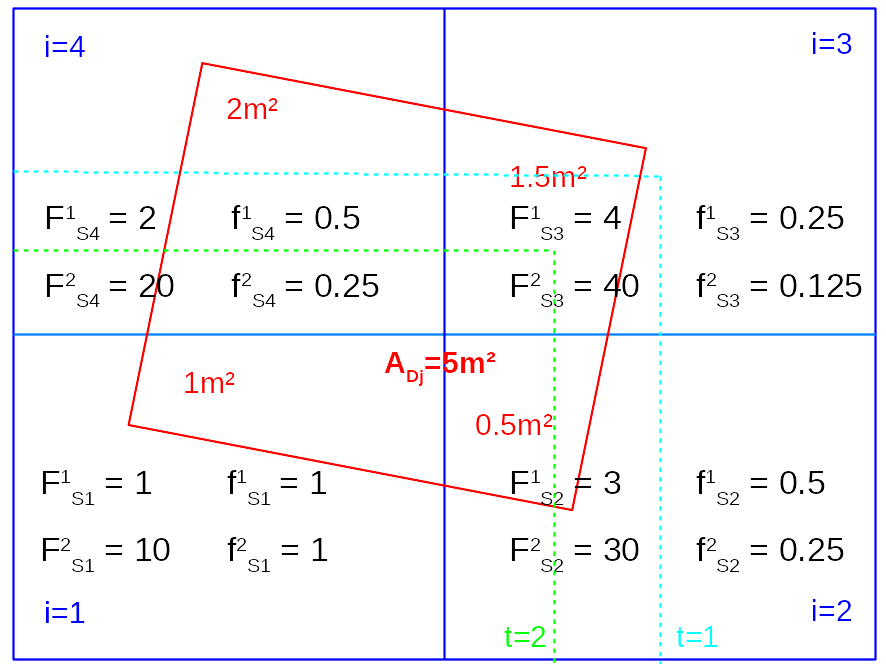
\includegraphics[width=0.75\linewidth]{figures/Fract_interp.png}
    \caption{Source and destination grids for the test case}
    \label{fig:test-case}
\end{figure}
The conservative remapping weights are therefore:\\
\(w_1 = 0.2\); 
\(w_2 = 0.1\);
\(w_3 = 0.3\);
\(w_4 = 0.4\)\\
At time 1, the active source surface covers the following fractions:\\
\(f^{1}_{S1} = 1.0\);
\(f^{1}_{S2} = 0.5\);
\(f^{1}_{S3} = 0.25\);
\(f^{1}_{S4} = 0.5\)\\
and the source fields is:\\
\(F^{1}_{S1} = 1.0\);
\(F^{1}_{S2} = 3.0\);
\(F^{1}_{S3} = 4.0\);
\(F^{1}_{S4} = 2.0\)\\
% Energy leaving source cells at t=1 : 1x1x1 + 3x0.5x0.5 + 4x0.25x1.5 + 2x0.5x2 = 5.25
% Energy leaving source cells at t=2 : 10x1x1 + 30x0.25x0.5 + 40x0.125x1.5 + 20x0.25x2 = 31.25
% Total energy : 36.50
If we neglected the sub-grid fractions, the remapped field at time 1 would be
\[F^{1}_{Dj}=\sum_i{w_iF^1_{Si}}=2.5\]
% 0.2x1 + 0.1x3 + 0.3x4 + 0.4x2 = 2.5
and it's contribution to the integral quantity on the destination grid would be
\[A_{Dj}F^{1}_{Dj}=12.5\]
% 5x2.5 = 12.5
If we take into consideration the source fractions, the destination scaled field as in eqn. (\ref{eqn:inst_scaled}) is
\[F^{1f}_{Dj} = \sum_iw_{i}f^1_{Si}F^1_{Si} = 1.05\]
%  0.2x1x1 + 0.1x0.5x3 + 0.3x0.25x4 + 0.4x0.5x2 = 1.05
It's contribution to the integral quantity on the destination grid is reduced to:
\[A_{Dj}F^{1f}_{Dj} = 5.25\]
% 5x1.05 = 5.25 OK
Taking into consideration the active destination surface coefficients as in eqn. (\ref{eqn:inst_dest_fract})
\[f^1_{Dj} = \sum_i{w_{i}f^1_{Si} = 0.525}\]
% 0.2x1 + 0.1x0.5 + 0.3x0.25 + 0.4x0.5 = 0.525
We can get the destination normalized scaled field as in eqn. (\ref{eqn:normalized_field})
\[F^{1fn}_{Dj} = \frac{F^{1f}_{Dj}}{f^1_{Dj}} = 2.0\]
% 1.05 / 0.525 = 2.0
and the active destination surface as in eqn. (\ref{eqn:active_dest_area})
\[A^{1a}_{Dj} = A_{Dj}f^1_{Dj} = 2.625\]
% 5 x 0.525 = 2.625
and find again the appropriate contribution to the integral quantity on the destination grid
\[A^{1a}_{Dj}F^{1fn}_{Dj} = 5.25\]
% 2.0 x 2.625 = 5.25 OK
\\
Let's now suppose that at time 2, the active source surface covers the following fractions:\\
\(f^{2}_{S1} = 1.0\);
\(f^{2}_{S2} = 0.25\);
\(f^{2}_{S3} = 0.125\);
\(f^{2}_{S4} = 0.25\)\\
and the source fields is:\\
\(F^{2}_{S1} = 10.0\);
\(F^{2}_{S2} = 30.0\);
\(F^{2}_{S3} = 40.0\);
\(F^{2}_{S4} = 20.0\)\\
\\
The instantaneous destination scaled field will then be:
\[F^{2f}_{Dj} = \sum_iw_{i}f^2_{Si}F^2_{Si} = 6.25\]
% 0.2x1x10 + 0.1x0.25x30 + 0.3x0.125x40 + 0.4x0.25x20 = 6.25
It's contribution to the integral quantity:
\[A_{Dj}F^{2f}_{Dj} = 31.25\]
% 5 x 6.25 = 31.25 OK
The active destination surface coefficient:
\[f^2_{Dj} = \sum_i{w_{i}f^2_{Si} = 0.3625}\]
% 0.2x1 + 0.1x0.25 + 0.3x0.125 + 0.4x0.25 = 0.3625
The destination normalized scaled field:
\[F^{2fn}_{Dj} = \frac{F^{2f}_{Dj}}{f^2_{Dj}} = 17.2414\]
% 6.25 / 0.3625 = 17.24137931
and the corresponding active destination surface :
\[A^{2a}_{Dj} = A_{Dj}f^2_{Dj} = 1.8125\]
% 5 x 0.3625 = 1.8125
which confirms the appropriate contribution:
\[A^{2a}_{Dj}F^{2fn}_{Dj} = 31.25\]
% 17.24137931 x 1.8125 = 31.25 OKe
\\
If we accumulate the field on the two time steps, neglecting the sub-grid fractions we obtain\\
\(F^{+}_{S1} = 11.0\);
% 1 + 10 = 11
\(F^{+}_{S2} = 33.0\);
% 3 + 30 = 33
\(F^{+}_{S3} = 44.0\);
% 4 + 40 = 44
\(F^{+}_{S4} = 22.0\)\\
% 2 + 20 = 22
and the destination accumulated field would be (equation \ref{destination_accumulated})
\[F^{+}_{Dj}=\sum_i{w_iF^{+}_{Si}}=27.5\]
% 0.2x11 + 0.1x33 + 0.3x44 + 0.4x22 = 27.5
Meanwhile, if we accumulate the scaled source fields we have\\
\(F^{+f}_{S1} = 11.0\);
% 1x1 + 10x1 = 11
\(F^{+f}_{S2} = 9.0\);
% 3x0.5 + 30x0.25 = 9
\(F^{+f}_{S3} = 6.0\);
% 4x0.25 + 40x0.125 = 6.0
\(F^{+f}_{S4} = 6.0\)\\
% 2x0.5 + 20x0.25 = 6.0
and the destination accumulated scaled field (equation \ref{eqn:nonnorm_accumulate_scaled}) has a much lower value:
\[F^{+f}_{Dj}=\sum_i{w_iF^{+f}_{Si}}=7.3\]
% 0.2x11 + 0.1x9 + 0.3x6 + 0.4x6 = 7.3
It's contribution to the integral quantity on the destination grid is:
\[A_{Dj}F^{+f}_{Dj} = 36.5\]
% 5 x 7.3 = 36.5
\\
We can obtain a more representative value by accumulating the instantaneous normalized scaled fields as in eqn. (\ref{eqn:accumulate_scaled})
\[F^{+fn}_{Dj}=\sum_t{\frac{F^{ft}_{Dj}}{f^t_{Dj}}}=19.24137931\]
% 1.05/0.525 + 6.25/0.3625 = 19.24137931
and derive its equivalent active destination cell fraction from eqn. (\ref{eqn:equivalent_dest_frac})
\[f^+_{Dj} = \frac{F^{+f}_{Dj}}{F^{+fn}_{Dj}} = 0.379390681\]
% 7.3 / 19.24137931 = 0.379390681
and an active surface:
\[A^a_{Dj}=A_{Dj}f^+_{Dj}=1.896953405\]
% 5 x 0.379390681 = 1.896953405
\\
Since the average values are just the half sum of the instantaneous values, the fractions are the same as in the accumulation case.\\
The averaged scaled source fields on the four cells are\\
\(\overline{F}^{f}_{S1} = 5.5\);
% (1x1 + 10x1)/2 = 5.5
\(\overline{F}^{f}_{S2} = 4.5\);
% (3x0.5 + 30x0.25)/2 = 4.5
\(\overline{F}^{f}_{S3} = 3.0\);
% (4x0.25 + 40x0.125)/2 = 3.0
\(\overline{F}^{f}_{S4} = 3.0\)\\
% (2x0.5 + 20x0.25)/2 = 3.0
The scaled remapped field is:
\[\overline{F}^{f}_{Dj}=\sum_i{w_i\overline{F}^{f}_{Si}}=3.65\]
% 0.2x5.5 + 0.1x4.5 + 0.3x3 + 0.4x3 = 3.65
It's contribution to the integral quantity on the destination grid is:
\[A_{Dj}\overline{F}^{f}_{Dj} = 18.25\]
% 5 x 3.65 = 18.25
\\
By averaging the normalized remapped values we obtain the more representative averaged field
\[\overline{F}^{fn}_{Dj}=9.620689655\]
and derive its equivalent active destination cell fraction 
\[\overline{f}_{Dj} = \frac{\overline{F}^{f}_{Dj}}{\overline{F}^{fn}_{Dj}} = 0.379390681\]
which is the same as in the accumulation case and implies an active surface:
\[A^a_{Dj}=A_{Dj}\overline{f}_{Dj}=1.896953405\]



%\include{UGA1_Grid_description}
\include{UGA4_changes}
%\include{UGA2_SCRIP}
%\include{UGA3_couplings}
%\include{UGA5_notinvolved}

\newpage
\begin{thebibliography}{10}
\vspace{-0.3cm}
\bibitem[{Cassou et~al 1998}]{cassou}
Cassou, C., P.~Noyret, E.~Sevault, O.~Thual, L.~Terray, D.~Beaucourt, and
  M.~Imbard:
\newblock Distributed Ocean-Atmosphere Modelling and Sensitivity to the
  Coupling Flux Precision: the CATHODe Project.
\newblock {\em Monthly Weather Review}, 126, No 4: 1035-1053, 1998.

\bibitem[{Chavas et~al 2013}]{chavas 13}
Chavas, J., E.~Audit, L.~Coquart, and S.~Valcke:
\newblock Conservative Regridding When Grid Cell Edges Are Unknown - Case of SCRIP
\newblock {\em Cerfacs Technical Report, TR-CMGC-13-6},
\newblock {\em Technical Report N$^o$ 0001, Maison de la Simulation, 91400 Saclay, France},
\newblock CECI, Universit\'e de Toulouse, CNRS, Toulouse, France

\bibitem[{Coquart et~al 2018}]{coquart 18}
Coquart, L., E.~Maisonnave, E. and S.~Valcke:
\newblock Using Open MP in OASIS3-MCT for the N-nearest-neighbor remapping
\newblock {\em Technical Report, WN/CMGC/18/19},
\newblock CECI, Universit\'e de Toulouse, CNRS, Toulouse, France

\bibitem[{Craig et~al 2017}]{craig17}
Craig, A., S.~Valcke and L.~Coquart :
\newblock Development and performance of a new version of the OASIS coupler, OASIS3-MCT\_3.0
\newblock {\em Geosci. Model Dev.}, 10: 3297--3308
\newblock https://doi.org/10.5194/gmd-10-3297-2017

\bibitem[{Craig et~al 2018}]{craig18}
Craig, A., S.~Valcke:
\newblock OASIS3-MCT4.0 Timing Study with MCT 2.10.beta1
\newblock {\em Technical Report, WN/CMGC/18/38},
\newblock CECI, Universit\'e de Toulouse, CNRS, Toulouse, France

\bibitem[{Craig 2019}]{craig19}
Craig, A. :
\newblock GSSPOS and BSSPOS options for the global conservation in OASIS3-MCT
\newblock {\em Technical Report, WN/CMGC/19/128},
\newblock CECI, Universit\'e de Toulouse, CNRS, Toulouse, France
\newblock https://oasis.cerfacs.fr/wp-content/uploads/sites/114/2021/08/GLOBC\_TR\_Craig\_oasis\_map\_conserv\_092019.pdf

\bibitem[{Guilyardi et~al 1995}]{guily95}
Guilyardi, E., G.~Madec, L.~Terray, M.~D\'equ\'e, M.~Pontaud, M.~Imbard, D.~Stephenson, M.-A. ~Filiberti, D.~Cariolle, P.~Delecluse, and O.~Thual.
\newblock Simulation coupl\'ee oc\'ean-atmosph\`ere de la variabilit\'e du climat.
\newblock {\em C.R. Acad. Sci. Paris}, t. 320, s\'erie IIa:683--690, 1995.

\bibitem[{He and Ding 2001}]{He2001}
He, Y. and C.~H.~Q Ding.
\newblock Using Accurate Arithmetics to Improve Numerical Reproducibility and Stability in Numer- ical Applications.
\newblock The Journal of Supercomputing, 18, 259
\newblock https://doi.org/10.1023/A:1008153532043, 2001.

\bibitem[{Jacob et~al 2005}]{mct_jacob}
Jacob, R., J.~Larson, and E.~Ong:
\newblock MxN Communication and Parallel Interpolation in CCSM3 Using the Model Coupling Toolkit.
\newblock {\em Int. J. High Perf. Comp. App.}, 19(3), 293-307 2005

\bibitem[{Jones 1999}]{Jones99}
Jones, P.:
\newblock Conservative remapping: First- and second-order conservative remapping.
\newblock Mon Weather Rev, 127, 2204-2210, 1999.

\bibitem[{Jonville and Valcke 2019}]{jonville2019}
Jonville, G. and S. Valcke:
\newblock Analysis of SCRIP conservative remapping in OASIS3-MCT –
Part B
\newblock {\em Technical Report, TR/CMGC/19/155},
\newblock CERFACS, Toulouse, France, 2020.
\newblock https://oasis.cerfacs.fr/wp-content/uploads/sites/114/2021/08/GLOBC\_TR\_Jonville-SCRIP\_CONSER\_TRNORM\_partB\_2019.pdf

\bibitem[{Larson et~al 2005}]{mct_larson}
Larson, J., R.~Jacob, and E.~Ong:
\newblock The Model Coupling Toolkit: A New Fortran90 Toolkit for Building Multiphysics Parallel Coupled Models.
\newblock {\em Int. J. High Perf. Comp. App.}, 19(3), 277-292, 2005

\bibitem[{Maisonnave 2020}]{maisonna2020}
Maisonnave, E.
\newblock Locally conservative OASIS interpolation using target grid nearest neighbours
\newblock {\em Technical Report, TR/CMGC/20/12},
\newblock CERFACS, Toulouse, France, 2020.
\newblock https://oasis.cerfacs.fr/wp-content/uploads/sites/114/2021/08/GLOBC\_TR\_Maisonnave-locally\_conserv\_interpolation\_2020.pdf

\bibitem[{Maisonnave et~al 2020}]{maisonnave20}
Maisonnave, E., L.~Coquart, and A.~Piacentini:
\newblock A better diagnostic of the load imbalance in OASIS based coupled systems
\newblock {\em Technical Report, TR/CMGC/20/176},
\newblock CERFACS, Toulouse, France, 2020.
\newblock https://oasis.cerfacs.fr/wp-content/uploads/sites/114/2021/08/GLOBC\_TR\_Maisonnave-load-balancing\_2020.pdf

\bibitem[{Mirin and Worley 2012}]{Mirin2012}
Mirin, A. A., and P.~H. Worley :
\newblock Improving the Per- formance Scalability of the Community Atmosphere Model.
\newblock {\em Int. J. High Perf. Comp. App.}, 26, 17–30
\newblock https://doi.org/10.1177/1094342011412630, 2012.

\bibitem[{Noyret et~al 1994}]{noyret}
Noyret, P., E.~Sevault, L.~Terray and O.~Thual.
\newblock Ocean-atmosphere coupling.
\newblock {\em Proceedings of the Fall Cray User Group (CUG) meeting},
1994.

\bibitem[{Piacentini et~al 2018}]{piacentini08}
Piacentini, A., E.~Maisonnave, G.~Jonville, L.~Coquart and S.~Valcke:
\newblock A parallel SCRIP interpolation library for OASIS,
\newblock {\em Technical Report, WN/CMGC/18/34},
\newblock CERFACS, Toulouse, France, 2018.
\newblock https://oasis.cerfacs.fr/wp-content/uploads/sites/114/2021/08/GLOBC\_WN\_Piacentini\_Parallel\_SCRIP\_cmgc\_18\_34\_2018.pdf

\bibitem[{Piacentini and Maisonnave 2020}]{piacentini20}
Piacentini, A. and E.~Maisonnave: 
\newblock Interactive visualisation of OASIS coupled models load imbalance
\newblock {\em Technical Report, TR/CMGC/20/177},
\newblock CERFACS, Toulouse, France, 2020.
\newblock https://oasis.cerfacs.fr/wp-content/uploads/sites/114/2021/08/GLOBC\_TR\_Piacentini\_Interactive\_visualisation\_of\_OASIS\_2020.pdf

\bibitem[{Pontaud et~al 1995}]{pontaud}
Pontaud, M., L.~Terray, E.~Guilyardi, E.~Sevault, D.~B. Stephenson, and
  O.~Thual.
\newblock Coupled ocean-atmosphere modelling - computing and scientific
  aspects.
\newblock In {\em 2nd UNAM-CRAY supercomputing conference, Numerical
  simulations in the environmental and earth sciences}
\newblock Mexico-city, Mexico, 1995.

 \bibitem[{Sevault et~al 1995}]{clim2}
Sevault, E., P.~Noyret, and L.~Terray.
\newblock Clim 1.2 user guide and reference manual.
\newblock {\em Technical Report TR/CGMC/95-47}, CERFACS, 1995.

\bibitem[{Terray and Thual 1995b}]{clim1}
Terray, L. and O.~Thual.
\newblock Oasis: le couplage oc\'ean-atmosph\`ere.
\newblock {\em La M\'et\'eorologie}, 10:50--61, 1995.

\bibitem[{Terray and Thual 1993}]{terray1}
Terray, L. and O.~Thual.
\newblock Coupled ocean-atmosphere simulations.
\newblock In {\em High Performance Computing in the Geosciences,
proceedings of the Les Houches Workshop}
\newblock F.X. Le Dimet Ed., Kluwer Academic Publishers B.V, 1993.

\bibitem[{Terray et~al 1995}]{clim3}
Terray, L., E.~Sevault, E.~Guilyardi and O.~Thual
\newblock OASIS 2.0 Ocean Atmosphere Sea Ice Soil User's Guide and Reference Manual
\newblock {\em Technical Report TR/CGMC/95-46}, CERFACS, 1995.

\bibitem[{Terray et~al 1995b}]{terray95}
Terray, L. O.~Thual, S.~Belamari, M.~D\'equ\'e, P.~Dandin, C.~L\'evy, and
P.~Delecluse.
\newblock Climatology and interannual variability simulated by the arpege-opa
model.
\newblock {\em Climate Dynamics}, 11:487--505, 1995

\bibitem[{Terray et~al 1999}]{terray3}
Terray, L., S.~Valcke and A.~Piacentini:
\newblock OASIS 2.3 Ocean Atmosphere Sea Ice Soil, User's Guide and
Reference Manual,
\newblock {\em Technical Report TR/CMGC/99-37},
\newblock CERFACS, Toulouse, France, 1999.

\bibitem[{Valcke et~al 2021}]{valcke21}
Valcke, S., Piacentini, A. and Jonville, G.
\newblock Benchmarking of regridding libraries used in Earth System
Modelling: SCRIP, YAC, ESMF and XIOS
\newblock {\em Technical Report, WN/CMGC/21/145},
\newblock CERFACS, Toulouse, France, 2021.
\newblock https XXXXXXXX

\bibitem[{Valcke and Piacentini 2019}]{valcke19}
Valcke, S. and A.~Piacentini
\newblock Analysis of SCRIP conservative remapping in OASIS3-MCT
\newblock {\em Technical Report, WN/CMGC/19/129},
\newblock CERFACS, Toulouse, France, 2019.
\newblock https://oasis.cerfacs.fr/wp-content/uploads/sites/114/2021/08/GLOBC\_TR\_Valcke-SCRIP\_CONSERV\_TRNORM\_partA\_2019.pdf

\bibitem[{Valcke et~al 2018}]{valcke11}
Valcke, S., L.~Coquart, A.~Craig, G.~Jonville, E.~Maisonnave, A.~Piacentini
\newblock Multithreaded or thread safe OASIS version including performance optimizations to adapt to many-core architectures, IS-ENES2 deliverable D2.3
\newblock {\em Technical Report, WN/CMGC/18/74},
\newblock CERFACS, Toulouse, France, 2018.

\bibitem[{Valcke et~al 2017}]{valcke12}
Valcke, S., G.~Jonville, R.~Ford, M.~Hobson, A.~Porter and G.~Riley
\newblock Report on benchmark suite for evaluation of coupling strategies
\newblock {\em Technical Report, TR/CMGC/17/87},
\newblock CERFACS, Toulouse, France, 2018.
\newblock http://cerfacs.fr/wp-content/uploads/2017/05/GLOBC-TR-IS-ENES2\_D10.3\_MAI2017.pdf

\bibitem[{Valcke et~al 2015}]{valcke10}
Valcke, S., T.~Craig, L.~Coquart:
\newblock OASIS3-MCT User Guide, OASIS3-MCT 3.0,
\newblock {\em Technical Report, WN/CMGC/15/38},
\newblock CERFACS, Toulouse, France, 2010.

\bibitem[{Valcke 2013}]{valcke9}
Valcke, S.:
\newblock The OASIS3 coupler: a European climate modelling community software
\newblock {\em Geosci. Model Dev.}, 6:373--388

\bibitem[{Valcke et~al 2013}]{valcke8}
Valcke, S., T.~Craig, L.~Coquart:
\newblock OASIS3-MCT User Guide, OASIS3-MCT 2.0,
\newblock {\em Technical Report, WN/CMGC/13/17},
\newblock CERFACS, Toulouse, France, 2013.

\bibitem[{Valcke et~al 2012}]{valcke7}
Valcke, S., T.~Craig, L.~Coquart:
\newblock OASIS3-MCT User Guide, OASIS3-MCT 1.0,
\newblock {\em Technical Report, WN/CMGC/12/49},
\newblock CERFACS, Toulouse, France, 2012.

\bibitem[{Valcke et~al 2011}]{valcke6}
Valcke, S., M.~Hanke, L.~Coquart:
\newblock OASIS4\_1 User Guide
\newblock {\em Technical Report TR/CMGC/11/50},
\newblock CERFACS, Toulouse, France, 2011.

\bibitem[{Valcke 2006b}]{valcke5}
Valcke, S.:
\newblock OASIS3 User Guide (prism\_2-5)
\newblock {\em Technical Report TR/CMGC/06/73},
\newblock CERFACS, Toulouse, France, 2006.

\bibitem[{Valcke 2006a}]{valcke4}
Valcke, S.:
\newblock OASIS4 User Guide (OASIS4\_0\_2),
\newblock {\em Technical Report TR/CMGC/06/74},
\newblock CERFACS, Toulouse, France, 2006.

\bibitem[{Valcke et~al 2004}]{valcke3}
Valcke, S., A.~Caubel, R.~Vogelsang, and D.~Declat:
\newblock OASIS3 User's Guide (oasis3\_prism\_2-4),
\newblock {\em PRISM Report No 2, 5th Ed.},
\newblock CERFACS, Toulouse, France, 2004.

\bibitem[{Valcke et~al 2003}]{valcke2}
Valcke, S., A.~Caubel, D.~Declat and L.~Terray:
\newblock OASIS3 Ocean Atmosphere Sea Ice Soil User's Guide,
\newblock {\em Technical Report TR/CMGC/03-69},
\newblock CERFACS, Toulouse, France, 2003.

\bibitem[{Valcke et~al 2000}]{valcke1}
Valcke, S., L.~Terray and A.~Piacentini:
\newblock OASIS 2.4 Ocean Atmosphere Sea Ice Soil, User's Guide and
Reference Manual,
\newblock {\em Technical Report TR/CMGC/00-10},
\newblock CERFACS, Toulouse, France, 2000.

\bibitem[{Voldoire 2020}]{voldoire2020}
Voldoire, A. 
\newblock River to ocean models interpolation
\newblock {\em Research Report},
\newblock CNRM, Universit{\'e} de Toulouse, M{\'e}t{\'e}o-France,
CNRS, Toulouse, France, 2020
\newblock https://hal-meteofrance.archives-ouvertes.fr/meteo-02986574/file/interpolation\_runoffs\_en.pdf

\end{thebibliography}

\end{document}
